\documentclass[twoside]{book}

% Packages required by doxygen
\usepackage{fixltx2e}
\usepackage{calc}
\usepackage{doxygen}
\usepackage[export]{adjustbox} % also loads graphicx
\usepackage{graphicx}
\usepackage[utf8]{inputenc}
\usepackage{makeidx}
\usepackage{multicol}
\usepackage{multirow}
\PassOptionsToPackage{warn}{textcomp}
\usepackage{textcomp}
\usepackage[nointegrals]{wasysym}
\usepackage[table]{xcolor}

% Font selection
\usepackage[T1]{fontenc}
\usepackage[scaled=.90]{helvet}
\usepackage{courier}
\usepackage{amssymb}
\usepackage{sectsty}
\renewcommand{\familydefault}{\sfdefault}
\allsectionsfont{%
  \fontseries{bc}\selectfont%
  \color{darkgray}%
}
\renewcommand{\DoxyLabelFont}{%
  \fontseries{bc}\selectfont%
  \color{darkgray}%
}
\newcommand{\+}{\discretionary{\mbox{\scriptsize$\hookleftarrow$}}{}{}}

% Page & text layout
\usepackage{geometry}
\geometry{%
  a4paper,%
  top=2.5cm,%
  bottom=2.5cm,%
  left=2.5cm,%
  right=2.5cm%
}
\tolerance=750
\hfuzz=15pt
\hbadness=750
\setlength{\emergencystretch}{15pt}
\setlength{\parindent}{0cm}
\setlength{\parskip}{3ex plus 2ex minus 2ex}
\makeatletter
\renewcommand{\paragraph}{%
  \@startsection{paragraph}{4}{0ex}{-1.0ex}{1.0ex}{%
    \normalfont\normalsize\bfseries\SS@parafont%
  }%
}
\renewcommand{\subparagraph}{%
  \@startsection{subparagraph}{5}{0ex}{-1.0ex}{1.0ex}{%
    \normalfont\normalsize\bfseries\SS@subparafont%
  }%
}
\makeatother

% Headers & footers
\usepackage{fancyhdr}
\pagestyle{fancyplain}
\fancyhead[LE]{\fancyplain{}{\bfseries\thepage}}
\fancyhead[CE]{\fancyplain{}{}}
\fancyhead[RE]{\fancyplain{}{\bfseries\leftmark}}
\fancyhead[LO]{\fancyplain{}{\bfseries\rightmark}}
\fancyhead[CO]{\fancyplain{}{}}
\fancyhead[RO]{\fancyplain{}{\bfseries\thepage}}
\fancyfoot[LE]{\fancyplain{}{}}
\fancyfoot[CE]{\fancyplain{}{}}
\fancyfoot[RE]{\fancyplain{}{\bfseries\scriptsize Generated by Doxygen }}
\fancyfoot[LO]{\fancyplain{}{\bfseries\scriptsize Generated by Doxygen }}
\fancyfoot[CO]{\fancyplain{}{}}
\fancyfoot[RO]{\fancyplain{}{}}
\renewcommand{\footrulewidth}{0.4pt}
\renewcommand{\chaptermark}[1]{%
  \markboth{#1}{}%
}
\renewcommand{\sectionmark}[1]{%
  \markright{\thesection\ #1}%
}

% Indices & bibliography
\usepackage{natbib}
\usepackage[titles]{tocloft}
\setcounter{tocdepth}{3}
\setcounter{secnumdepth}{5}
\makeindex

% Hyperlinks (required, but should be loaded last)
\usepackage{ifpdf}
\ifpdf
  \usepackage[pdftex,pagebackref=true]{hyperref}
\else
  \usepackage[ps2pdf,pagebackref=true]{hyperref}
\fi
\hypersetup{%
  colorlinks=true,%
  linkcolor=blue,%
  citecolor=blue,%
  unicode%
}

% Custom commands
\newcommand{\clearemptydoublepage}{%
  \newpage{\pagestyle{empty}\cleardoublepage}%
}

\usepackage{caption}
\captionsetup{labelsep=space,justification=centering,font={bf},singlelinecheck=off,skip=4pt,position=top}

%===== C O N T E N T S =====

\begin{document}

% Titlepage & ToC
\hypersetup{pageanchor=false,
             bookmarksnumbered=true,
             pdfencoding=unicode
            }
\pagenumbering{alph}
\begin{titlepage}
\vspace*{7cm}
\begin{center}%
{\Large osu\+\_\+iforest }\\
\vspace*{1cm}
{\large Generated by Doxygen 1.8.14}\\
\end{center}
\end{titlepage}
\clearemptydoublepage
\pagenumbering{roman}
\tableofcontents
\clearemptydoublepage
\pagenumbering{arabic}
\hypersetup{pageanchor=true}

%--- Begin generated contents ---
\chapter{Namespace Index}
\section{Namespace List}
Here is a list of all namespaces with brief descriptions\+:\begin{DoxyCompactList}
\item\contentsline{section}{\hyperlink{namespacemetric}{metric} }{\pageref{namespacemetric}}{}
\item\contentsline{section}{\hyperlink{namespaceutil}{util} }{\pageref{namespaceutil}}{}
\end{DoxyCompactList}

\chapter{Hierarchical Index}
\section{Class Hierarchy}
This inheritance list is sorted roughly, but not completely, alphabetically\+:\begin{DoxyCompactList}
\item \contentsline{section}{Bootstrap\+Convergence}{\pageref{classBootstrapConvergence}}{}
\item \contentsline{section}{Contrib}{\pageref{structContrib}}{}
\item enable\+\_\+shared\+\_\+from\+\_\+this\begin{DoxyCompactList}
\item \contentsline{section}{Tree}{\pageref{classTree}}{}
\end{DoxyCompactList}
\item \contentsline{section}{Forest}{\pageref{classForest}}{}
\begin{DoxyCompactList}
\item \contentsline{section}{conv\+Forest}{\pageref{classconvForest}}{}
\item \contentsline{section}{Isolation\+Forest}{\pageref{classIsolationForest}}{}
\item \contentsline{section}{R\+Forest}{\pageref{classRForest}}{}
\end{DoxyCompactList}
\item \contentsline{section}{Forest\+:\+:larger}{\pageref{structForest_1_1larger}}{}
\item \contentsline{section}{conv\+Forest\+:\+:larger}{\pageref{structconvForest_1_1larger}}{}
\item \contentsline{section}{util\+:\+:Matrix$<$ T $>$}{\pageref{classutil_1_1Matrix}}{}
\item \contentsline{section}{util\+:\+:Matrix$<$ bool $>$}{\pageref{classutil_1_1Matrix}}{}
\item \contentsline{section}{O\+O\+B\+Estimator}{\pageref{structOOBEstimator}}{}
\item \contentsline{section}{smaller}{\pageref{structsmaller}}{}
\item \contentsline{section}{conv\+Forest\+:\+:topscore}{\pageref{structconvForest_1_1topscore}}{}
\end{DoxyCompactList}

\chapter{Data Structure Index}
\section{Data Structures}
Here are the data structures with brief descriptions\+:\begin{DoxyCompactList}
\item\contentsline{section}{\hyperlink{classBootstrapConvergence}{Bootstrap\+Convergence} }{\pageref{classBootstrapConvergence}}{}
\item\contentsline{section}{\hyperlink{structContrib}{Contrib} }{\pageref{structContrib}}{}
\item\contentsline{section}{\hyperlink{classconvForest}{conv\+Forest} }{\pageref{classconvForest}}{}
\item\contentsline{section}{\hyperlink{classForest}{Forest} }{\pageref{classForest}}{}
\item\contentsline{section}{\hyperlink{classIsolationForest}{Isolation\+Forest} }{\pageref{classIsolationForest}}{}
\item\contentsline{section}{\hyperlink{structForest_1_1larger}{Forest\+::larger} }{\pageref{structForest_1_1larger}}{}
\item\contentsline{section}{\hyperlink{structconvForest_1_1larger}{conv\+Forest\+::larger} }{\pageref{structconvForest_1_1larger}}{}
\item\contentsline{section}{\hyperlink{classutil_1_1Matrix}{util\+::\+Matrix$<$ T $>$} }{\pageref{classutil_1_1Matrix}}{}
\item\contentsline{section}{\hyperlink{structOOBEstimator}{O\+O\+B\+Estimator} }{\pageref{structOOBEstimator}}{}
\item\contentsline{section}{\hyperlink{classRForest}{R\+Forest} }{\pageref{classRForest}}{}
\item\contentsline{section}{\hyperlink{structsmaller}{smaller} }{\pageref{structsmaller}}{}
\item\contentsline{section}{\hyperlink{structconvForest_1_1topscore}{conv\+Forest\+::topscore} }{\pageref{structconvForest_1_1topscore}}{}
\item\contentsline{section}{\hyperlink{classTree}{Tree} }{\pageref{classTree}}{}
\end{DoxyCompactList}

\chapter{File Index}
\section{File List}
Here is a list of all files with brief descriptions\+:\begin{DoxyCompactList}
\item\contentsline{section}{src/\hyperlink{BootstrapConvergence_8cpp}{Bootstrap\+Convergence.\+cpp} }{\pageref{BootstrapConvergence_8cpp}}{}
\item\contentsline{section}{src/\hyperlink{BootstrapConvergence_8hpp}{Bootstrap\+Convergence.\+hpp} }{\pageref{BootstrapConvergence_8hpp}}{}
\item\contentsline{section}{src/\hyperlink{cincl_8hpp}{cincl.\+hpp} }{\pageref{cincl_8hpp}}{}
\item\contentsline{section}{src/\hyperlink{Contribution_8hpp}{Contribution.\+hpp} }{\pageref{Contribution_8hpp}}{}
\item\contentsline{section}{src/\hyperlink{convForest_8cpp}{conv\+Forest.\+cpp} }{\pageref{convForest_8cpp}}{}
\item\contentsline{section}{src/\hyperlink{convForest_8hpp}{conv\+Forest.\+hpp} }{\pageref{convForest_8hpp}}{}
\item\contentsline{section}{src/\hyperlink{Forest_8cpp}{Forest.\+cpp} }{\pageref{Forest_8cpp}}{}
\item\contentsline{section}{src/\hyperlink{Forest_8hpp}{Forest.\+hpp} }{\pageref{Forest_8hpp}}{}
\item\contentsline{section}{src/\hyperlink{IsolationForest_8cpp}{Isolation\+Forest.\+cpp} }{\pageref{IsolationForest_8cpp}}{}
\item\contentsline{section}{src/\hyperlink{IsolationForest_8hpp}{Isolation\+Forest.\+hpp} }{\pageref{IsolationForest_8hpp}}{}
\item\contentsline{section}{src/\hyperlink{main_8hpp}{main.\+hpp} }{\pageref{main_8hpp}}{}
\item\contentsline{section}{src/\hyperlink{metric_8cpp}{metric.\+cpp} }{\pageref{metric_8cpp}}{}
\item\contentsline{section}{src/\hyperlink{metric_8hpp}{metric.\+hpp} }{\pageref{metric_8hpp}}{}
\item\contentsline{section}{src/\hyperlink{OOBEstimator_8hpp}{O\+O\+B\+Estimator.\+hpp} }{\pageref{OOBEstimator_8hpp}}{}
\item\contentsline{section}{src/\hyperlink{RForest_8cpp}{R\+Forest.\+cpp} }{\pageref{RForest_8cpp}}{}
\item\contentsline{section}{src/\hyperlink{RForest_8hpp}{R\+Forest.\+hpp} }{\pageref{RForest_8hpp}}{}
\item\contentsline{section}{src/\hyperlink{Tree_8cpp}{Tree.\+cpp} }{\pageref{Tree_8cpp}}{}
\item\contentsline{section}{src/\hyperlink{Tree_8hpp}{Tree.\+hpp} }{\pageref{Tree_8hpp}}{}
\item\contentsline{section}{src/\hyperlink{utility_8cpp}{utility.\+cpp} }{\pageref{utility_8cpp}}{}
\item\contentsline{section}{src/\hyperlink{utility_8hpp}{utility.\+hpp} }{\pageref{utility_8hpp}}{}
\end{DoxyCompactList}

\chapter{Namespace Documentation}
\hypertarget{namespacemetric}{}\section{metric Namespace Reference}
\label{namespacemetric}\index{metric@{metric}}
\subsection*{Functions}
\begin{DoxyCompactItemize}
\item 
double \hyperlink{namespacemetric_a87e5308fcebc95b5720c24dc70d74349}{trapezoid\+Area} (double X1, double X2, double Y1, double Y2)
\item 
double \hyperlink{namespacemetric_a57492bb556d712873ca231e6427a139e}{A\+UC} (vector$<$ double $>$ \&labels, vector$<$ double $>$ \&scores, int n, int posclass)
\item 
double \hyperlink{namespacemetric_af2bf0a8c7be4bee4eff0abaa603e842e}{A\+UC} (std\+::vector$<$ double $>$ \&labels, std\+::vector$<$ double $>$ \&scores, int n, int posclass)
\item 
double \hyperlink{namespacemetric_a3db123a20e7cf257d2c3777be1573094}{ap} (std\+::vector$<$ double $>$ \&labels, std\+::vector$<$ double $>$ \&scores, int n, int posclass)
\end{DoxyCompactItemize}


\subsection{Function Documentation}
\mbox{\Hypertarget{namespacemetric_a3db123a20e7cf257d2c3777be1573094}\label{namespacemetric_a3db123a20e7cf257d2c3777be1573094}} 
\index{metric@{metric}!ap@{ap}}
\index{ap@{ap}!metric@{metric}}
\subsubsection{\texorpdfstring{ap()}{ap()}}
{\footnotesize\ttfamily double metric\+::ap (\begin{DoxyParamCaption}\item[{std\+::vector$<$ double $>$ \&}]{labels,  }\item[{std\+::vector$<$ double $>$ \&}]{scores,  }\item[{int}]{n,  }\item[{int}]{posclass }\end{DoxyParamCaption})}

\mbox{\Hypertarget{namespacemetric_a57492bb556d712873ca231e6427a139e}\label{namespacemetric_a57492bb556d712873ca231e6427a139e}} 
\index{metric@{metric}!A\+UC@{A\+UC}}
\index{A\+UC@{A\+UC}!metric@{metric}}
\subsubsection{\texorpdfstring{A\+U\+C()}{AUC()}\hspace{0.1cm}{\footnotesize\ttfamily [1/2]}}
{\footnotesize\ttfamily double metric\+::\+A\+UC (\begin{DoxyParamCaption}\item[{vector$<$ double $>$ \&}]{labels,  }\item[{vector$<$ double $>$ \&}]{scores,  }\item[{int}]{n,  }\item[{int}]{posclass }\end{DoxyParamCaption})}

\mbox{\Hypertarget{namespacemetric_af2bf0a8c7be4bee4eff0abaa603e842e}\label{namespacemetric_af2bf0a8c7be4bee4eff0abaa603e842e}} 
\index{metric@{metric}!A\+UC@{A\+UC}}
\index{A\+UC@{A\+UC}!metric@{metric}}
\subsubsection{\texorpdfstring{A\+U\+C()}{AUC()}\hspace{0.1cm}{\footnotesize\ttfamily [2/2]}}
{\footnotesize\ttfamily double metric\+::\+A\+UC (\begin{DoxyParamCaption}\item[{std\+::vector$<$ double $>$ \&}]{labels,  }\item[{std\+::vector$<$ double $>$ \&}]{scores,  }\item[{int}]{n,  }\item[{int}]{posclass }\end{DoxyParamCaption})}

\mbox{\Hypertarget{namespacemetric_a87e5308fcebc95b5720c24dc70d74349}\label{namespacemetric_a87e5308fcebc95b5720c24dc70d74349}} 
\index{metric@{metric}!trapezoid\+Area@{trapezoid\+Area}}
\index{trapezoid\+Area@{trapezoid\+Area}!metric@{metric}}
\subsubsection{\texorpdfstring{trapezoid\+Area()}{trapezoidArea()}}
{\footnotesize\ttfamily double metric\+::trapezoid\+Area (\begin{DoxyParamCaption}\item[{double}]{X1,  }\item[{double}]{X2,  }\item[{double}]{Y1,  }\item[{double}]{Y2 }\end{DoxyParamCaption})}


\hypertarget{namespaceutil}{}\section{util Namespace Reference}
\label{namespaceutil}\index{util@{util}}
\subsection*{Data Structures}
\begin{DoxyCompactItemize}
\item 
class \hyperlink{classutil_1_1Matrix}{Matrix}
\end{DoxyCompactItemize}
\subsection*{Functions}
\begin{DoxyCompactItemize}
\item 
void \hyperlink{namespaceutil_a60fc54ed78936dca89472845766b61f8}{initialize} ()
\item 
{\footnotesize template$<$typename T $>$ }\\T \hyperlink{namespaceutil_a254d46b3ebe9a685b6e0eca9db9d51ec}{randomT} (T min, T max)
\item 
double \hyperlink{namespaceutil_a1327645fe6fef26083bc9e1185b8d586}{randomD} (double min, double max)
\item 
int \hyperlink{namespaceutil_ab473893d6b386b2da951b72b4d40c085}{randomI} (int min, int max)
\item 
int \hyperlink{namespaceutil_a8751577b60f8e83b41c3cca32d65b677}{random\+Ex} (int min, int max, set$<$ int $>$ \&exlude)
\item 
void \hyperlink{namespaceutil_ab4e338c554526c6a942fc35d14b15beb}{sampleI} (int min, int max, int nsample, vector$<$ int $>$ \&samples)
\item 
double \hyperlink{namespaceutil_a71809e272f5a9c8e8297bab2c12666f7}{score} (double depth, int n)
\item 
{\footnotesize template$<$typename T $>$ }\\void \hyperlink{namespaceutil_a998845d03758baa45e52b967cf230b01}{swap\+Int} (int a, int b, T $\ast$x)
\item 
double \hyperlink{namespaceutil_afded8090794a80d2f1c9aa44e70c85ff}{mean} (vector$<$ double $>$ points)
\item 
double \hyperlink{namespaceutil_a43a50c7b5c6674cd27461d91cfec686c}{variance} (vector$<$ double $>$ \&x)
\item 
double \hyperlink{namespaceutil_a68758b62ab028fd0a2f0afb6d516be6f}{tconf} (vector$<$ double $>$ \&points, double sigma=0.\+95)
\item 
vector$<$ vector$<$ double $>$ $>$ \hyperlink{namespaceutil_a84b10f9fb76cc3f825e8c680ca7d786e}{readcsv} (const char $\ast$filename, char delim=\textquotesingle{},\textquotesingle{}, bool header=true)
\item 
map$<$ double, double $>$ \hyperlink{namespaceutil_ac7478c2543d3bf4901961c719ecc7d04}{ecdf} (vector$<$ double $>$ points)
\item 
{\footnotesize template$<$typename T $>$ }\\vector$<$ T $>$ \hyperlink{namespaceutil_a3da5afd362118ed04ca18ec46d5e6a96}{flatten} (const vector$<$ vector$<$ T $>$$>$ \&v)
\item 
double \hyperlink{namespaceutil_a1f106b9a1a65806393f73a3c8dbf01a6}{avg\+PL} (int n)
\item 
vector$<$ double $>$ \hyperlink{namespaceutil_a422abe670c555eeeded897e3d9861b77}{A\+Ddistance} (vector$<$ vector$<$ double $>$ $>$ depths, bool weight\+To\+Tail=false)
\item 
int \hyperlink{namespaceutil_ae080f004741b0ea81032b3ec0c723f4c}{random\+Ex} (int min, int max, std\+::set$<$ int $>$ \&exlude)
\item 
void \hyperlink{namespaceutil_a077f5faad89062a4013dc98fc85b7a40}{sampleI} (int min, int max, int nsample, std\+::vector$<$ int $>$ \&sample\+Indx)
\item 
void \hyperlink{namespaceutil_a8a222a481a56e4070f023d369483f707}{swap\+Int} (int a, int b, int $\ast$x)
\item 
double \hyperlink{namespaceutil_a2f9d2ca343c1e5fcbc1da5140de61f94}{variance} (std\+::vector$<$ double $>$ \&x)
\item 
double \hyperlink{namespaceutil_a67baa21858f5d569c1553bb179da7115}{mean} (std\+::vector$<$ double $>$ points)
\item 
double \hyperlink{namespaceutil_a0b673442b1c87f0daf8bb0a4179a6834}{tconf} (std\+::vector$<$ double $>$ \&points, double sigma)
\item 
std\+::map$<$ double, double $>$ \hyperlink{namespaceutil_abfb0e38d71ca69f5f6a505b3f5f7dc52}{ecdf} (std\+::vector$<$ double $>$ points)
\item 
std\+::vector$<$ double $>$ \hyperlink{namespaceutil_a08fbdd196c73244d0e2130c3a70d2f2b}{A\+Ddistance} (const std\+::vector$<$ std\+::vector$<$ double $>$ $>$ \&depths, bool weight\+To\+Tail)
\end{DoxyCompactItemize}
\subsection*{Variables}
\begin{DoxyCompactItemize}
\item 
default\+\_\+random\+\_\+engine \hyperlink{namespaceutil_ab30b96cc3fcd37942fb7f9f8a2e1898d}{gen}
\item 
std\+::ofstream \hyperlink{namespaceutil_af123fd54ef9ea843e69a69dfd986f59e}{logfile}
\item 
std\+::string \hyperlink{namespaceutil_a4839a6e82a650d17fe48a7ab99640835}{tmp\+Var}
\item 
int \hyperlink{namespaceutil_aeda4e5339822ac6c9fb3f1991c126bfb}{debug}
\end{DoxyCompactItemize}


\subsection{Function Documentation}
\mbox{\Hypertarget{namespaceutil_a08fbdd196c73244d0e2130c3a70d2f2b}\label{namespaceutil_a08fbdd196c73244d0e2130c3a70d2f2b}} 
\index{util@{util}!A\+Ddistance@{A\+Ddistance}}
\index{A\+Ddistance@{A\+Ddistance}!util@{util}}
\subsubsection{\texorpdfstring{A\+Ddistance()}{ADdistance()}\hspace{0.1cm}{\footnotesize\ttfamily [1/2]}}
{\footnotesize\ttfamily std\+::vector$<$double$>$ util\+::\+A\+Ddistance (\begin{DoxyParamCaption}\item[{const std\+::vector$<$ std\+::vector$<$ double $>$ $>$ \&}]{depths,  }\item[{bool}]{weight\+To\+Tail }\end{DoxyParamCaption})}

\mbox{\Hypertarget{namespaceutil_a422abe670c555eeeded897e3d9861b77}\label{namespaceutil_a422abe670c555eeeded897e3d9861b77}} 
\index{util@{util}!A\+Ddistance@{A\+Ddistance}}
\index{A\+Ddistance@{A\+Ddistance}!util@{util}}
\subsubsection{\texorpdfstring{A\+Ddistance()}{ADdistance()}\hspace{0.1cm}{\footnotesize\ttfamily [2/2]}}
{\footnotesize\ttfamily vector$<$double$>$ util\+::\+A\+Ddistance (\begin{DoxyParamCaption}\item[{vector$<$ vector$<$ double $>$ $>$}]{depths,  }\item[{bool}]{weight\+To\+Tail = {\ttfamily false} }\end{DoxyParamCaption})}

\mbox{\Hypertarget{namespaceutil_a1f106b9a1a65806393f73a3c8dbf01a6}\label{namespaceutil_a1f106b9a1a65806393f73a3c8dbf01a6}} 
\index{util@{util}!avg\+PL@{avg\+PL}}
\index{avg\+PL@{avg\+PL}!util@{util}}
\subsubsection{\texorpdfstring{avg\+P\+L()}{avgPL()}}
{\footnotesize\ttfamily double util\+::avg\+PL (\begin{DoxyParamCaption}\item[{int}]{n }\end{DoxyParamCaption})}

\mbox{\Hypertarget{namespaceutil_abfb0e38d71ca69f5f6a505b3f5f7dc52}\label{namespaceutil_abfb0e38d71ca69f5f6a505b3f5f7dc52}} 
\index{util@{util}!ecdf@{ecdf}}
\index{ecdf@{ecdf}!util@{util}}
\subsubsection{\texorpdfstring{ecdf()}{ecdf()}\hspace{0.1cm}{\footnotesize\ttfamily [1/2]}}
{\footnotesize\ttfamily std\+::map$<$double,double$>$ util\+::ecdf (\begin{DoxyParamCaption}\item[{std\+::vector$<$ double $>$}]{points }\end{DoxyParamCaption})}

\mbox{\Hypertarget{namespaceutil_ac7478c2543d3bf4901961c719ecc7d04}\label{namespaceutil_ac7478c2543d3bf4901961c719ecc7d04}} 
\index{util@{util}!ecdf@{ecdf}}
\index{ecdf@{ecdf}!util@{util}}
\subsubsection{\texorpdfstring{ecdf()}{ecdf()}\hspace{0.1cm}{\footnotesize\ttfamily [2/2]}}
{\footnotesize\ttfamily map$<$double,double$>$ util\+::ecdf (\begin{DoxyParamCaption}\item[{vector$<$ double $>$}]{points }\end{DoxyParamCaption})}

\mbox{\Hypertarget{namespaceutil_a3da5afd362118ed04ca18ec46d5e6a96}\label{namespaceutil_a3da5afd362118ed04ca18ec46d5e6a96}} 
\index{util@{util}!flatten@{flatten}}
\index{flatten@{flatten}!util@{util}}
\subsubsection{\texorpdfstring{flatten()}{flatten()}}
{\footnotesize\ttfamily template$<$typename T $>$ \\
vector$<$T$>$ util\+::flatten (\begin{DoxyParamCaption}\item[{const vector$<$ vector$<$ T $>$$>$ \&}]{v }\end{DoxyParamCaption})}

\mbox{\Hypertarget{namespaceutil_a60fc54ed78936dca89472845766b61f8}\label{namespaceutil_a60fc54ed78936dca89472845766b61f8}} 
\index{util@{util}!initialize@{initialize}}
\index{initialize@{initialize}!util@{util}}
\subsubsection{\texorpdfstring{initialize()}{initialize()}}
{\footnotesize\ttfamily void util\+::initialize (\begin{DoxyParamCaption}{ }\end{DoxyParamCaption})}

\mbox{\Hypertarget{namespaceutil_a67baa21858f5d569c1553bb179da7115}\label{namespaceutil_a67baa21858f5d569c1553bb179da7115}} 
\index{util@{util}!mean@{mean}}
\index{mean@{mean}!util@{util}}
\subsubsection{\texorpdfstring{mean()}{mean()}\hspace{0.1cm}{\footnotesize\ttfamily [1/2]}}
{\footnotesize\ttfamily double util\+::mean (\begin{DoxyParamCaption}\item[{std\+::vector$<$ double $>$}]{points }\end{DoxyParamCaption})}

\mbox{\Hypertarget{namespaceutil_afded8090794a80d2f1c9aa44e70c85ff}\label{namespaceutil_afded8090794a80d2f1c9aa44e70c85ff}} 
\index{util@{util}!mean@{mean}}
\index{mean@{mean}!util@{util}}
\subsubsection{\texorpdfstring{mean()}{mean()}\hspace{0.1cm}{\footnotesize\ttfamily [2/2]}}
{\footnotesize\ttfamily double util\+::mean (\begin{DoxyParamCaption}\item[{vector$<$ double $>$}]{points }\end{DoxyParamCaption})}

\mbox{\Hypertarget{namespaceutil_a1327645fe6fef26083bc9e1185b8d586}\label{namespaceutil_a1327645fe6fef26083bc9e1185b8d586}} 
\index{util@{util}!randomD@{randomD}}
\index{randomD@{randomD}!util@{util}}
\subsubsection{\texorpdfstring{random\+D()}{randomD()}}
{\footnotesize\ttfamily double util\+::randomD (\begin{DoxyParamCaption}\item[{double}]{min,  }\item[{double}]{max }\end{DoxyParamCaption})}

\mbox{\Hypertarget{namespaceutil_ae080f004741b0ea81032b3ec0c723f4c}\label{namespaceutil_ae080f004741b0ea81032b3ec0c723f4c}} 
\index{util@{util}!random\+Ex@{random\+Ex}}
\index{random\+Ex@{random\+Ex}!util@{util}}
\subsubsection{\texorpdfstring{random\+Ex()}{randomEx()}\hspace{0.1cm}{\footnotesize\ttfamily [1/2]}}
{\footnotesize\ttfamily int util\+::random\+Ex (\begin{DoxyParamCaption}\item[{int}]{min,  }\item[{int}]{max,  }\item[{std\+::set$<$ int $>$ \&}]{exlude }\end{DoxyParamCaption})}

\mbox{\Hypertarget{namespaceutil_a8751577b60f8e83b41c3cca32d65b677}\label{namespaceutil_a8751577b60f8e83b41c3cca32d65b677}} 
\index{util@{util}!random\+Ex@{random\+Ex}}
\index{random\+Ex@{random\+Ex}!util@{util}}
\subsubsection{\texorpdfstring{random\+Ex()}{randomEx()}\hspace{0.1cm}{\footnotesize\ttfamily [2/2]}}
{\footnotesize\ttfamily int util\+::random\+Ex (\begin{DoxyParamCaption}\item[{int}]{min,  }\item[{int}]{max,  }\item[{set$<$ int $>$ \&}]{exlude }\end{DoxyParamCaption})}

\mbox{\Hypertarget{namespaceutil_ab473893d6b386b2da951b72b4d40c085}\label{namespaceutil_ab473893d6b386b2da951b72b4d40c085}} 
\index{util@{util}!randomI@{randomI}}
\index{randomI@{randomI}!util@{util}}
\subsubsection{\texorpdfstring{random\+I()}{randomI()}}
{\footnotesize\ttfamily int util\+::randomI (\begin{DoxyParamCaption}\item[{int}]{min,  }\item[{int}]{max }\end{DoxyParamCaption})}

\mbox{\Hypertarget{namespaceutil_a254d46b3ebe9a685b6e0eca9db9d51ec}\label{namespaceutil_a254d46b3ebe9a685b6e0eca9db9d51ec}} 
\index{util@{util}!randomT@{randomT}}
\index{randomT@{randomT}!util@{util}}
\subsubsection{\texorpdfstring{random\+T()}{randomT()}}
{\footnotesize\ttfamily template$<$typename T $>$ \\
T util\+::randomT (\begin{DoxyParamCaption}\item[{T}]{min,  }\item[{T}]{max }\end{DoxyParamCaption})}

\mbox{\Hypertarget{namespaceutil_a84b10f9fb76cc3f825e8c680ca7d786e}\label{namespaceutil_a84b10f9fb76cc3f825e8c680ca7d786e}} 
\index{util@{util}!readcsv@{readcsv}}
\index{readcsv@{readcsv}!util@{util}}
\subsubsection{\texorpdfstring{readcsv()}{readcsv()}}
{\footnotesize\ttfamily std\+::vector$<$ std\+::vector$<$ double $>$ $>$ util\+::readcsv (\begin{DoxyParamCaption}\item[{const char $\ast$}]{filename,  }\item[{char}]{delim = {\ttfamily \textquotesingle{},\textquotesingle{}},  }\item[{bool}]{header = {\ttfamily true} }\end{DoxyParamCaption})}

\mbox{\Hypertarget{namespaceutil_a077f5faad89062a4013dc98fc85b7a40}\label{namespaceutil_a077f5faad89062a4013dc98fc85b7a40}} 
\index{util@{util}!sampleI@{sampleI}}
\index{sampleI@{sampleI}!util@{util}}
\subsubsection{\texorpdfstring{sample\+I()}{sampleI()}\hspace{0.1cm}{\footnotesize\ttfamily [1/2]}}
{\footnotesize\ttfamily void util\+::sampleI (\begin{DoxyParamCaption}\item[{int}]{min,  }\item[{int}]{max,  }\item[{int}]{nsample,  }\item[{std\+::vector$<$ int $>$ \&}]{sample\+Indx }\end{DoxyParamCaption})}

\mbox{\Hypertarget{namespaceutil_ab4e338c554526c6a942fc35d14b15beb}\label{namespaceutil_ab4e338c554526c6a942fc35d14b15beb}} 
\index{util@{util}!sampleI@{sampleI}}
\index{sampleI@{sampleI}!util@{util}}
\subsubsection{\texorpdfstring{sample\+I()}{sampleI()}\hspace{0.1cm}{\footnotesize\ttfamily [2/2]}}
{\footnotesize\ttfamily void util\+::sampleI (\begin{DoxyParamCaption}\item[{int}]{min,  }\item[{int}]{max,  }\item[{int}]{nsample,  }\item[{vector$<$ int $>$ \&}]{samples }\end{DoxyParamCaption})}

\mbox{\Hypertarget{namespaceutil_a71809e272f5a9c8e8297bab2c12666f7}\label{namespaceutil_a71809e272f5a9c8e8297bab2c12666f7}} 
\index{util@{util}!score@{score}}
\index{score@{score}!util@{util}}
\subsubsection{\texorpdfstring{score()}{score()}}
{\footnotesize\ttfamily double util\+::score (\begin{DoxyParamCaption}\item[{double}]{depth,  }\item[{int}]{n }\end{DoxyParamCaption})}

\mbox{\Hypertarget{namespaceutil_a8a222a481a56e4070f023d369483f707}\label{namespaceutil_a8a222a481a56e4070f023d369483f707}} 
\index{util@{util}!swap\+Int@{swap\+Int}}
\index{swap\+Int@{swap\+Int}!util@{util}}
\subsubsection{\texorpdfstring{swap\+Int()}{swapInt()}\hspace{0.1cm}{\footnotesize\ttfamily [1/2]}}
{\footnotesize\ttfamily void util\+::swap\+Int (\begin{DoxyParamCaption}\item[{int}]{a,  }\item[{int}]{b,  }\item[{int $\ast$}]{x }\end{DoxyParamCaption})}

\mbox{\Hypertarget{namespaceutil_a998845d03758baa45e52b967cf230b01}\label{namespaceutil_a998845d03758baa45e52b967cf230b01}} 
\index{util@{util}!swap\+Int@{swap\+Int}}
\index{swap\+Int@{swap\+Int}!util@{util}}
\subsubsection{\texorpdfstring{swap\+Int()}{swapInt()}\hspace{0.1cm}{\footnotesize\ttfamily [2/2]}}
{\footnotesize\ttfamily template$<$typename T $>$ \\
void util\+::swap\+Int (\begin{DoxyParamCaption}\item[{int}]{a,  }\item[{int}]{b,  }\item[{T $\ast$}]{x }\end{DoxyParamCaption})}

\mbox{\Hypertarget{namespaceutil_a0b673442b1c87f0daf8bb0a4179a6834}\label{namespaceutil_a0b673442b1c87f0daf8bb0a4179a6834}} 
\index{util@{util}!tconf@{tconf}}
\index{tconf@{tconf}!util@{util}}
\subsubsection{\texorpdfstring{tconf()}{tconf()}\hspace{0.1cm}{\footnotesize\ttfamily [1/2]}}
{\footnotesize\ttfamily double util\+::tconf (\begin{DoxyParamCaption}\item[{std\+::vector$<$ double $>$ \&}]{points,  }\item[{double}]{sigma }\end{DoxyParamCaption})}

\mbox{\Hypertarget{namespaceutil_a68758b62ab028fd0a2f0afb6d516be6f}\label{namespaceutil_a68758b62ab028fd0a2f0afb6d516be6f}} 
\index{util@{util}!tconf@{tconf}}
\index{tconf@{tconf}!util@{util}}
\subsubsection{\texorpdfstring{tconf()}{tconf()}\hspace{0.1cm}{\footnotesize\ttfamily [2/2]}}
{\footnotesize\ttfamily double util\+::tconf (\begin{DoxyParamCaption}\item[{vector$<$ double $>$ \&}]{points,  }\item[{double}]{sigma = {\ttfamily 0.95} }\end{DoxyParamCaption})}

\mbox{\Hypertarget{namespaceutil_a2f9d2ca343c1e5fcbc1da5140de61f94}\label{namespaceutil_a2f9d2ca343c1e5fcbc1da5140de61f94}} 
\index{util@{util}!variance@{variance}}
\index{variance@{variance}!util@{util}}
\subsubsection{\texorpdfstring{variance()}{variance()}\hspace{0.1cm}{\footnotesize\ttfamily [1/2]}}
{\footnotesize\ttfamily double util\+::variance (\begin{DoxyParamCaption}\item[{std\+::vector$<$ double $>$ \&}]{x }\end{DoxyParamCaption})}

\mbox{\Hypertarget{namespaceutil_a43a50c7b5c6674cd27461d91cfec686c}\label{namespaceutil_a43a50c7b5c6674cd27461d91cfec686c}} 
\index{util@{util}!variance@{variance}}
\index{variance@{variance}!util@{util}}
\subsubsection{\texorpdfstring{variance()}{variance()}\hspace{0.1cm}{\footnotesize\ttfamily [2/2]}}
{\footnotesize\ttfamily double util\+::variance (\begin{DoxyParamCaption}\item[{vector$<$ double $>$ \&}]{x }\end{DoxyParamCaption})}



\subsection{Variable Documentation}
\mbox{\Hypertarget{namespaceutil_aeda4e5339822ac6c9fb3f1991c126bfb}\label{namespaceutil_aeda4e5339822ac6c9fb3f1991c126bfb}} 
\index{util@{util}!debug@{debug}}
\index{debug@{debug}!util@{util}}
\subsubsection{\texorpdfstring{debug}{debug}}
{\footnotesize\ttfamily int util\+::debug}

\mbox{\Hypertarget{namespaceutil_ab30b96cc3fcd37942fb7f9f8a2e1898d}\label{namespaceutil_ab30b96cc3fcd37942fb7f9f8a2e1898d}} 
\index{util@{util}!gen@{gen}}
\index{gen@{gen}!util@{util}}
\subsubsection{\texorpdfstring{gen}{gen}}
{\footnotesize\ttfamily default\+\_\+random\+\_\+engine util\+::gen}

\mbox{\Hypertarget{namespaceutil_af123fd54ef9ea843e69a69dfd986f59e}\label{namespaceutil_af123fd54ef9ea843e69a69dfd986f59e}} 
\index{util@{util}!logfile@{logfile}}
\index{logfile@{logfile}!util@{util}}
\subsubsection{\texorpdfstring{logfile}{logfile}}
{\footnotesize\ttfamily std\+::ofstream util\+::logfile}

\mbox{\Hypertarget{namespaceutil_a4839a6e82a650d17fe48a7ab99640835}\label{namespaceutil_a4839a6e82a650d17fe48a7ab99640835}} 
\index{util@{util}!tmp\+Var@{tmp\+Var}}
\index{tmp\+Var@{tmp\+Var}!util@{util}}
\subsubsection{\texorpdfstring{tmp\+Var}{tmpVar}}
{\footnotesize\ttfamily std\+::string util\+::tmp\+Var}


\chapter{Data Structure Documentation}
\hypertarget{classBootstrapConvergence}{}\section{Bootstrap\+Convergence Class Reference}
\label{classBootstrapConvergence}\index{Bootstrap\+Convergence@{Bootstrap\+Convergence}}


{\ttfamily \#include $<$Bootstrap\+Convergence.\+hpp$>$}



Collaboration diagram for Bootstrap\+Convergence\+:\nopagebreak
\begin{figure}[H]
\begin{center}
\leavevmode
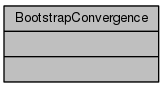
\includegraphics[width=194pt]{classBootstrapConvergence__coll__graph}
\end{center}
\end{figure}


The documentation for this class was generated from the following file\+:\begin{DoxyCompactItemize}
\item 
src/\hyperlink{BootstrapConvergence_8hpp}{Bootstrap\+Convergence.\+hpp}\end{DoxyCompactItemize}

\hypertarget{structContrib}{}\section{Contrib Struct Reference}
\label{structContrib}\index{Contrib@{Contrib}}


{\ttfamily \#include $<$Contribution.\+hpp$>$}



Collaboration diagram for Contrib\+:\nopagebreak
\begin{figure}[H]
\begin{center}
\leavevmode
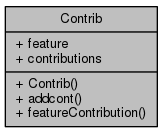
\includegraphics[width=194pt]{structContrib__coll__graph}
\end{center}
\end{figure}
\subsection*{Public Member Functions}
\begin{DoxyCompactItemize}
\item 
\hyperlink{structContrib_af03799ba9bb8cf2a603d334d1be68780}{Contrib} (int ncols)
\item 
void \hyperlink{structContrib_a03900805a2d1b5452f62d347511bec90}{addcont} (int index, double depth)
\item 
std\+::map$<$ int, double $>$ \hyperlink{structContrib_ab3a6d22d834b8fa669b436672d21dd0b}{feature\+Contribution} ()
\end{DoxyCompactItemize}
\subsection*{Data Fields}
\begin{DoxyCompactItemize}
\item 
int \hyperlink{structContrib_ad6106fc9377c5d7025631449db2e322c}{feature}
\item 
std\+::map$<$ int, std\+::vector$<$ double $>$ $>$ \hyperlink{structContrib_adfd8e1bb6847746d18bdeced40876b59}{contributions}
\end{DoxyCompactItemize}


\subsection{Constructor \& Destructor Documentation}
\mbox{\Hypertarget{structContrib_af03799ba9bb8cf2a603d334d1be68780}\label{structContrib_af03799ba9bb8cf2a603d334d1be68780}} 
\index{Contrib@{Contrib}!Contrib@{Contrib}}
\index{Contrib@{Contrib}!Contrib@{Contrib}}
\subsubsection{\texorpdfstring{Contrib()}{Contrib()}}
{\footnotesize\ttfamily Contrib\+::\+Contrib (\begin{DoxyParamCaption}\item[{int}]{ncols }\end{DoxyParamCaption})\hspace{0.3cm}{\ttfamily [inline]}}



\subsection{Member Function Documentation}
\mbox{\Hypertarget{structContrib_a03900805a2d1b5452f62d347511bec90}\label{structContrib_a03900805a2d1b5452f62d347511bec90}} 
\index{Contrib@{Contrib}!addcont@{addcont}}
\index{addcont@{addcont}!Contrib@{Contrib}}
\subsubsection{\texorpdfstring{addcont()}{addcont()}}
{\footnotesize\ttfamily void Contrib\+::addcont (\begin{DoxyParamCaption}\item[{int}]{index,  }\item[{double}]{depth }\end{DoxyParamCaption})\hspace{0.3cm}{\ttfamily [inline]}}

\mbox{\Hypertarget{structContrib_ab3a6d22d834b8fa669b436672d21dd0b}\label{structContrib_ab3a6d22d834b8fa669b436672d21dd0b}} 
\index{Contrib@{Contrib}!feature\+Contribution@{feature\+Contribution}}
\index{feature\+Contribution@{feature\+Contribution}!Contrib@{Contrib}}
\subsubsection{\texorpdfstring{feature\+Contribution()}{featureContribution()}}
{\footnotesize\ttfamily std\+::map$<$int,double$>$ Contrib\+::feature\+Contribution (\begin{DoxyParamCaption}{ }\end{DoxyParamCaption})\hspace{0.3cm}{\ttfamily [inline]}}



\subsection{Field Documentation}
\mbox{\Hypertarget{structContrib_adfd8e1bb6847746d18bdeced40876b59}\label{structContrib_adfd8e1bb6847746d18bdeced40876b59}} 
\index{Contrib@{Contrib}!contributions@{contributions}}
\index{contributions@{contributions}!Contrib@{Contrib}}
\subsubsection{\texorpdfstring{contributions}{contributions}}
{\footnotesize\ttfamily std\+::map$<$int,std\+::vector$<$double$>$ $>$ Contrib\+::contributions}

\mbox{\Hypertarget{structContrib_ad6106fc9377c5d7025631449db2e322c}\label{structContrib_ad6106fc9377c5d7025631449db2e322c}} 
\index{Contrib@{Contrib}!feature@{feature}}
\index{feature@{feature}!Contrib@{Contrib}}
\subsubsection{\texorpdfstring{feature}{feature}}
{\footnotesize\ttfamily int Contrib\+::feature}



The documentation for this struct was generated from the following file\+:\begin{DoxyCompactItemize}
\item 
src/\hyperlink{Contribution_8hpp}{Contribution.\+hpp}\end{DoxyCompactItemize}

\hypertarget{classconvForest}{}\section{conv\+Forest Class Reference}
\label{classconvForest}\index{conv\+Forest@{conv\+Forest}}


{\ttfamily \#include $<$conv\+Forest.\+hpp$>$}



Inheritance diagram for conv\+Forest\+:\nopagebreak
\begin{figure}[H]
\begin{center}
\leavevmode
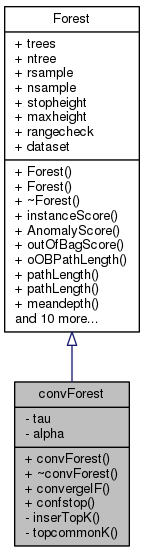
\includegraphics[width=180pt]{classconvForest__inherit__graph}
\end{center}
\end{figure}


Collaboration diagram for conv\+Forest\+:\nopagebreak
\begin{figure}[H]
\begin{center}
\leavevmode
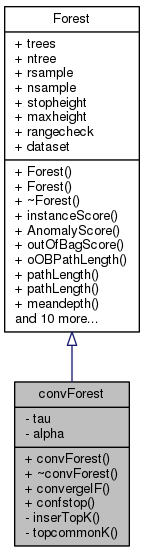
\includegraphics[width=180pt]{classconvForest__coll__graph}
\end{center}
\end{figure}
\subsection*{Data Structures}
\begin{DoxyCompactItemize}
\item 
struct \hyperlink{structconvForest_1_1larger}{larger}
\item 
struct \hyperlink{structconvForest_1_1topscore}{topscore}
\end{DoxyCompactItemize}
\subsection*{Public Member Functions}
\begin{DoxyCompactItemize}
\item 
\hyperlink{classconvForest_a03387416058b37c24de2d7a901275695}{conv\+Forest} (int \+\_\+ntree, doubleframe $\ast$\+\_\+df, const int \+\_\+nsample, int \+\_\+maxheight, bool \+\_\+stopheight, bool \+\_\+rsample, double \+\_\+tau, double \+\_\+alpha)
\item 
virtual \hyperlink{classconvForest_a85d5cb4ec991893853acf4be144cdf52}{$\sim$conv\+Forest} ()=default
\item 
void \hyperlink{classconvForest_acf0da12a09b3aa4323c4dc3fe6f1be56}{converge\+IF} (double \hyperlink{classconvForest_a390216111823cd05c48aad3a358a49a7}{tau}, double \hyperlink{classconvForest_a69ed3ccc19fa0439f9fb64ce28c3c66f}{alpha})
\item 
void \hyperlink{classconvForest_a4a20fbcf944458fbbc62400bc0bb2de7}{confstop} (double \hyperlink{classconvForest_a69ed3ccc19fa0439f9fb64ce28c3c66f}{alpha})
\end{DoxyCompactItemize}
\subsection*{Private Member Functions}
\begin{DoxyCompactItemize}
\item 
void \hyperlink{classconvForest_a64930c8a4d1e1f74fc45f3ce5c24a55e}{inser\+TopK} (std\+::vector$<$ std\+::pair$<$ int, int $>$ $>$ \&sl, int b)
\item 
double \hyperlink{classconvForest_a650511b77be61f6c5766fcd6b577b33e}{topcommonK} (std\+::vector$<$ int $>$ \&v1, std\+::vector$<$ int $>$ \&v2)
\end{DoxyCompactItemize}
\subsection*{Private Attributes}
\begin{DoxyCompactItemize}
\item 
int \hyperlink{classconvForest_a390216111823cd05c48aad3a358a49a7}{tau}
\item 
int \hyperlink{classconvForest_a69ed3ccc19fa0439f9fb64ce28c3c66f}{alpha}
\end{DoxyCompactItemize}
\subsection*{Additional Inherited Members}


\subsection{Constructor \& Destructor Documentation}
\mbox{\Hypertarget{classconvForest_a03387416058b37c24de2d7a901275695}\label{classconvForest_a03387416058b37c24de2d7a901275695}} 
\index{conv\+Forest@{conv\+Forest}!conv\+Forest@{conv\+Forest}}
\index{conv\+Forest@{conv\+Forest}!conv\+Forest@{conv\+Forest}}
\subsubsection{\texorpdfstring{conv\+Forest()}{convForest()}}
{\footnotesize\ttfamily conv\+Forest\+::conv\+Forest (\begin{DoxyParamCaption}\item[{int}]{\+\_\+ntree,  }\item[{doubleframe $\ast$}]{\+\_\+df,  }\item[{const int}]{\+\_\+nsample,  }\item[{int}]{\+\_\+maxheight,  }\item[{bool}]{\+\_\+stopheight,  }\item[{bool}]{\+\_\+rsample,  }\item[{double}]{\+\_\+tau,  }\item[{double}]{\+\_\+alpha }\end{DoxyParamCaption})\hspace{0.3cm}{\ttfamily [inline]}}

\mbox{\Hypertarget{classconvForest_a85d5cb4ec991893853acf4be144cdf52}\label{classconvForest_a85d5cb4ec991893853acf4be144cdf52}} 
\index{conv\+Forest@{conv\+Forest}!````~conv\+Forest@{$\sim$conv\+Forest}}
\index{````~conv\+Forest@{$\sim$conv\+Forest}!conv\+Forest@{conv\+Forest}}
\subsubsection{\texorpdfstring{$\sim$conv\+Forest()}{~convForest()}}
{\footnotesize\ttfamily virtual conv\+Forest\+::$\sim$conv\+Forest (\begin{DoxyParamCaption}{ }\end{DoxyParamCaption})\hspace{0.3cm}{\ttfamily [virtual]}, {\ttfamily [default]}}



\subsection{Member Function Documentation}
\mbox{\Hypertarget{classconvForest_a4a20fbcf944458fbbc62400bc0bb2de7}\label{classconvForest_a4a20fbcf944458fbbc62400bc0bb2de7}} 
\index{conv\+Forest@{conv\+Forest}!confstop@{confstop}}
\index{confstop@{confstop}!conv\+Forest@{conv\+Forest}}
\subsubsection{\texorpdfstring{confstop()}{confstop()}}
{\footnotesize\ttfamily void conv\+Forest\+::confstop (\begin{DoxyParamCaption}\item[{double}]{alpha }\end{DoxyParamCaption})}

\mbox{\Hypertarget{classconvForest_acf0da12a09b3aa4323c4dc3fe6f1be56}\label{classconvForest_acf0da12a09b3aa4323c4dc3fe6f1be56}} 
\index{conv\+Forest@{conv\+Forest}!converge\+IF@{converge\+IF}}
\index{converge\+IF@{converge\+IF}!conv\+Forest@{conv\+Forest}}
\subsubsection{\texorpdfstring{converge\+I\+F()}{convergeIF()}}
{\footnotesize\ttfamily void conv\+Forest\+::converge\+IF (\begin{DoxyParamCaption}\item[{double}]{tau,  }\item[{double}]{alpha }\end{DoxyParamCaption})}

\mbox{\Hypertarget{classconvForest_a64930c8a4d1e1f74fc45f3ce5c24a55e}\label{classconvForest_a64930c8a4d1e1f74fc45f3ce5c24a55e}} 
\index{conv\+Forest@{conv\+Forest}!inser\+TopK@{inser\+TopK}}
\index{inser\+TopK@{inser\+TopK}!conv\+Forest@{conv\+Forest}}
\subsubsection{\texorpdfstring{inser\+Top\+K()}{inserTopK()}}
{\footnotesize\ttfamily void conv\+Forest\+::inser\+TopK (\begin{DoxyParamCaption}\item[{std\+::vector$<$ std\+::pair$<$ int, int $>$ $>$ \&}]{sl,  }\item[{int}]{b }\end{DoxyParamCaption})\hspace{0.3cm}{\ttfamily [private]}}

\mbox{\Hypertarget{classconvForest_a650511b77be61f6c5766fcd6b577b33e}\label{classconvForest_a650511b77be61f6c5766fcd6b577b33e}} 
\index{conv\+Forest@{conv\+Forest}!topcommonK@{topcommonK}}
\index{topcommonK@{topcommonK}!conv\+Forest@{conv\+Forest}}
\subsubsection{\texorpdfstring{topcommon\+K()}{topcommonK()}}
{\footnotesize\ttfamily double conv\+Forest\+::topcommonK (\begin{DoxyParamCaption}\item[{std\+::vector$<$ int $>$ \&}]{v1,  }\item[{std\+::vector$<$ int $>$ \&}]{v2 }\end{DoxyParamCaption})\hspace{0.3cm}{\ttfamily [private]}}



\subsection{Field Documentation}
\mbox{\Hypertarget{classconvForest_a69ed3ccc19fa0439f9fb64ce28c3c66f}\label{classconvForest_a69ed3ccc19fa0439f9fb64ce28c3c66f}} 
\index{conv\+Forest@{conv\+Forest}!alpha@{alpha}}
\index{alpha@{alpha}!conv\+Forest@{conv\+Forest}}
\subsubsection{\texorpdfstring{alpha}{alpha}}
{\footnotesize\ttfamily int conv\+Forest\+::alpha\hspace{0.3cm}{\ttfamily [private]}}

\mbox{\Hypertarget{classconvForest_a390216111823cd05c48aad3a358a49a7}\label{classconvForest_a390216111823cd05c48aad3a358a49a7}} 
\index{conv\+Forest@{conv\+Forest}!tau@{tau}}
\index{tau@{tau}!conv\+Forest@{conv\+Forest}}
\subsubsection{\texorpdfstring{tau}{tau}}
{\footnotesize\ttfamily int conv\+Forest\+::tau\hspace{0.3cm}{\ttfamily [private]}}



The documentation for this class was generated from the following files\+:\begin{DoxyCompactItemize}
\item 
src/\hyperlink{convForest_8hpp}{conv\+Forest.\+hpp}\item 
src/\hyperlink{convForest_8cpp}{conv\+Forest.\+cpp}\end{DoxyCompactItemize}

\hypertarget{classForest}{}\section{Forest Class Reference}
\label{classForest}\index{Forest@{Forest}}


{\ttfamily \#include $<$Forest.\+hpp$>$}



Inheritance diagram for Forest\+:\nopagebreak
\begin{figure}[H]
\begin{center}
\leavevmode
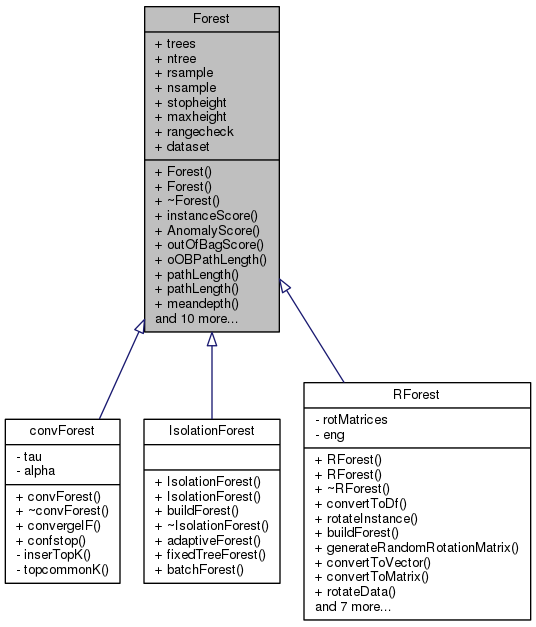
\includegraphics[width=350pt]{classForest__inherit__graph}
\end{center}
\end{figure}


Collaboration diagram for Forest\+:\nopagebreak
\begin{figure}[H]
\begin{center}
\leavevmode
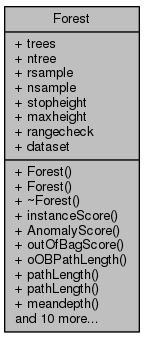
\includegraphics[width=180pt]{classForest__coll__graph}
\end{center}
\end{figure}
\subsection*{Data Structures}
\begin{DoxyCompactItemize}
\item 
struct \hyperlink{structForest_1_1larger}{larger}
\end{DoxyCompactItemize}
\subsection*{Public Member Functions}
\begin{DoxyCompactItemize}
\item 
\hyperlink{classForest_af9ad2787ae306cb4da8d7443da124d15}{Forest} ()
\item 
\hyperlink{classForest_ab5be587f4e0768155c39a9bc8484bc57}{Forest} (int \+\_\+ntree, doubleframe $\ast$\+\_\+dataset, int \+\_\+nsample, int \+\_\+maxheight, bool \+\_\+stopheight, bool \+\_\+rsample)
\item 
virtual \hyperlink{classForest_a5ae182b3027fb3be4f1f5c76388ea211}{$\sim$\+Forest} ()=default
\item 
double \hyperlink{classForest_ac88b19d31bc5cc92b429af2716b81325}{instance\+Score} (double $\ast$inst)
\item 
std\+::vector$<$ double $>$ \hyperlink{classForest_a39c34e59ac0088959ce86ddd6bacf9f1}{Anomaly\+Score} (doubleframe $\ast$df)
\item 
std\+::vector$<$ double $>$ \hyperlink{classForest_abc30331242d62253818f72585f757502}{out\+Of\+Bag\+Score} (doubleframe $\ast$df)
\item 
std\+::vector$<$ std\+::vector$<$ double $>$ $>$ \hyperlink{classForest_a2ec4ab1b6cec96a7492a6a8b25a7075d}{o\+O\+B\+Path\+Length} (doubleframe $\ast$data)
\item 
virtual std\+::vector$<$ double $>$ \hyperlink{classForest_a8e3bac70e9f10ce6f301e297e32e8f5a}{path\+Length} (double $\ast$inst)
\item 
std\+::vector$<$ std\+::vector$<$ double $>$ $>$ \hyperlink{classForest_af031c54e9e04b11c21c2b629d6bd0c5c}{path\+Length} (doubleframe $\ast$data)
\item 
std\+::vector$<$ double $>$ \hyperlink{classForest_ac30644f1c7bfc633005875b845e9cd8a}{meandepth} ()
\item 
std\+::vector$<$ double $>$ \hyperlink{classForest_a695e24a0ca4a1a5685f4ab1eb996984c}{A\+Dtest} (const std\+::vector$<$ std\+::vector$<$ double $>$ $>$ \&pathlength, bool weighttotail)
\item 
std\+::map$<$ int, double $>$ \hyperlink{classForest_acb23b1464f1244ad49e178935485384c}{importance} (double $\ast$inst)
\item 
virtual double \hyperlink{classForest_a977abbe81e409465546cef0164b5b439}{getdepth} (double $\ast$inst, std\+::shared\+\_\+ptr$<$ \hyperlink{classTree}{Tree} $>$ tree)
\item 
void \hyperlink{classForest_aaa05ed85d49d7b465e518e62f1393210}{get\+Sample} (std\+::vector$<$ int $>$ \&sample\+Index, const int \hyperlink{classForest_a3a9831dba286e35fbe1f46ad9d363bf4}{nsample}, bool r\+Sample, int nrow)
\item 
virtual int \hyperlink{classForest_a825bb350730c50aa8924e9f761c4a2a4}{adaptive\+Forest} (double alpha, int stop\+Limit)
\item 
virtual void \hyperlink{classForest_a0699073aa8d6b46fdbdc36b7299a1a34}{fixed\+Tree\+Forest} (int epoch)
\item 
virtual int \hyperlink{classForest_aa2b99dda19e39783a6da9de8fa318ceb}{conf\+Tree} (double alpha, double rho, int init\+\_\+tree)
\item 
double \hyperlink{classForest_a43ce9dc43658d70521aa2aee91b9a60a}{topcommonK} (std\+::vector$<$ int $>$ \&v1, std\+::vector$<$ int $>$ \&v2)
\item 
virtual std\+::vector$<$ std\+::map$<$ int, double $>$ $>$ \hyperlink{classForest_a1c17fba4c766d0dbd41df7a050b1fa81}{feature\+Contrib} (double $\ast$inst)
\item 
void \hyperlink{classForest_abcae06f2a9b350eac3f8617ac7bc9e1a}{feature\+Explanation} (doubleframe $\ast$df, std\+::ofstream \&out)
\end{DoxyCompactItemize}
\subsection*{Data Fields}
\begin{DoxyCompactItemize}
\item 
std\+::vector$<$ std\+::shared\+\_\+ptr$<$ \hyperlink{classTree}{Tree} $>$ $>$ \hyperlink{classForest_acbfc6b953ce79295ecc9646fdb52e917}{trees}
\item 
int \hyperlink{classForest_a63aab05561b82d08972ee8fe455c45cc}{ntree}
\item 
bool \hyperlink{classForest_a64b54558dfe88223f0521443c0b34b17}{rsample}
\item 
int \hyperlink{classForest_a3a9831dba286e35fbe1f46ad9d363bf4}{nsample}
\item 
bool \hyperlink{classForest_a066998b292bc6c764b7244830f027631}{stopheight}
\item 
int \hyperlink{classForest_a296ffbe5ca7db543740dda34c71771f5}{maxheight}
\item 
bool \hyperlink{classForest_a590efbd7b01fa3fdb023d10df3d9792b}{rangecheck}
\item 
doubleframe $\ast$ \hyperlink{classForest_ac3704ed2300734a73cba5b04a8f4b6ae}{dataset}
\end{DoxyCompactItemize}


\subsection{Constructor \& Destructor Documentation}
\mbox{\Hypertarget{classForest_af9ad2787ae306cb4da8d7443da124d15}\label{classForest_af9ad2787ae306cb4da8d7443da124d15}} 
\index{Forest@{Forest}!Forest@{Forest}}
\index{Forest@{Forest}!Forest@{Forest}}
\subsubsection{\texorpdfstring{Forest()}{Forest()}\hspace{0.1cm}{\footnotesize\ttfamily [1/2]}}
{\footnotesize\ttfamily Forest\+::\+Forest (\begin{DoxyParamCaption}{ }\end{DoxyParamCaption})\hspace{0.3cm}{\ttfamily [inline]}}

\mbox{\Hypertarget{classForest_ab5be587f4e0768155c39a9bc8484bc57}\label{classForest_ab5be587f4e0768155c39a9bc8484bc57}} 
\index{Forest@{Forest}!Forest@{Forest}}
\index{Forest@{Forest}!Forest@{Forest}}
\subsubsection{\texorpdfstring{Forest()}{Forest()}\hspace{0.1cm}{\footnotesize\ttfamily [2/2]}}
{\footnotesize\ttfamily Forest\+::\+Forest (\begin{DoxyParamCaption}\item[{int}]{\+\_\+ntree,  }\item[{doubleframe $\ast$}]{\+\_\+dataset,  }\item[{int}]{\+\_\+nsample,  }\item[{int}]{\+\_\+maxheight,  }\item[{bool}]{\+\_\+stopheight,  }\item[{bool}]{\+\_\+rsample }\end{DoxyParamCaption})\hspace{0.3cm}{\ttfamily [inline]}}

\mbox{\Hypertarget{classForest_a5ae182b3027fb3be4f1f5c76388ea211}\label{classForest_a5ae182b3027fb3be4f1f5c76388ea211}} 
\index{Forest@{Forest}!````~Forest@{$\sim$\+Forest}}
\index{````~Forest@{$\sim$\+Forest}!Forest@{Forest}}
\subsubsection{\texorpdfstring{$\sim$\+Forest()}{~Forest()}}
{\footnotesize\ttfamily virtual Forest\+::$\sim$\+Forest (\begin{DoxyParamCaption}{ }\end{DoxyParamCaption})\hspace{0.3cm}{\ttfamily [virtual]}, {\ttfamily [default]}}



\subsection{Member Function Documentation}
\mbox{\Hypertarget{classForest_a825bb350730c50aa8924e9f761c4a2a4}\label{classForest_a825bb350730c50aa8924e9f761c4a2a4}} 
\index{Forest@{Forest}!adaptive\+Forest@{adaptive\+Forest}}
\index{adaptive\+Forest@{adaptive\+Forest}!Forest@{Forest}}
\subsubsection{\texorpdfstring{adaptive\+Forest()}{adaptiveForest()}}
{\footnotesize\ttfamily int Forest\+::adaptive\+Forest (\begin{DoxyParamCaption}\item[{double}]{alpha,  }\item[{int}]{stop\+Limit }\end{DoxyParamCaption})\hspace{0.3cm}{\ttfamily [virtual]}}



Reimplemented in \hyperlink{classRForest_abc389cab7fa7ffee669b3add5aad4c52}{R\+Forest}, and \hyperlink{classIsolationForest_a33dae487524bd1fdaf085a36dab04ee9}{Isolation\+Forest}.

\mbox{\Hypertarget{classForest_a695e24a0ca4a1a5685f4ab1eb996984c}\label{classForest_a695e24a0ca4a1a5685f4ab1eb996984c}} 
\index{Forest@{Forest}!A\+Dtest@{A\+Dtest}}
\index{A\+Dtest@{A\+Dtest}!Forest@{Forest}}
\subsubsection{\texorpdfstring{A\+Dtest()}{ADtest()}}
{\footnotesize\ttfamily std\+::vector$<$double$>$ Forest\+::\+A\+Dtest (\begin{DoxyParamCaption}\item[{const std\+::vector$<$ std\+::vector$<$ double $>$ $>$ \&}]{pathlength,  }\item[{bool}]{weighttotail }\end{DoxyParamCaption})}

\mbox{\Hypertarget{classForest_a39c34e59ac0088959ce86ddd6bacf9f1}\label{classForest_a39c34e59ac0088959ce86ddd6bacf9f1}} 
\index{Forest@{Forest}!Anomaly\+Score@{Anomaly\+Score}}
\index{Anomaly\+Score@{Anomaly\+Score}!Forest@{Forest}}
\subsubsection{\texorpdfstring{Anomaly\+Score()}{AnomalyScore()}}
{\footnotesize\ttfamily std\+::vector$<$ double $>$ Forest\+::\+Anomaly\+Score (\begin{DoxyParamCaption}\item[{doubleframe $\ast$}]{df }\end{DoxyParamCaption})}

\mbox{\Hypertarget{classForest_aa2b99dda19e39783a6da9de8fa318ceb}\label{classForest_aa2b99dda19e39783a6da9de8fa318ceb}} 
\index{Forest@{Forest}!conf\+Tree@{conf\+Tree}}
\index{conf\+Tree@{conf\+Tree}!Forest@{Forest}}
\subsubsection{\texorpdfstring{conf\+Tree()}{confTree()}}
{\footnotesize\ttfamily int Forest\+::conf\+Tree (\begin{DoxyParamCaption}\item[{double}]{alpha,  }\item[{double}]{rho,  }\item[{int}]{init\+\_\+tree }\end{DoxyParamCaption})\hspace{0.3cm}{\ttfamily [virtual]}}

\mbox{\Hypertarget{classForest_a1c17fba4c766d0dbd41df7a050b1fa81}\label{classForest_a1c17fba4c766d0dbd41df7a050b1fa81}} 
\index{Forest@{Forest}!feature\+Contrib@{feature\+Contrib}}
\index{feature\+Contrib@{feature\+Contrib}!Forest@{Forest}}
\subsubsection{\texorpdfstring{feature\+Contrib()}{featureContrib()}}
{\footnotesize\ttfamily std\+::vector$<$ std\+::map$<$ int, double $>$ $>$ Forest\+::feature\+Contrib (\begin{DoxyParamCaption}\item[{double $\ast$}]{inst }\end{DoxyParamCaption})\hspace{0.3cm}{\ttfamily [virtual]}}

\mbox{\Hypertarget{classForest_abcae06f2a9b350eac3f8617ac7bc9e1a}\label{classForest_abcae06f2a9b350eac3f8617ac7bc9e1a}} 
\index{Forest@{Forest}!feature\+Explanation@{feature\+Explanation}}
\index{feature\+Explanation@{feature\+Explanation}!Forest@{Forest}}
\subsubsection{\texorpdfstring{feature\+Explanation()}{featureExplanation()}}
{\footnotesize\ttfamily void Forest\+::feature\+Explanation (\begin{DoxyParamCaption}\item[{doubleframe $\ast$}]{df,  }\item[{std\+::ofstream \&}]{out }\end{DoxyParamCaption})}

\mbox{\Hypertarget{classForest_a0699073aa8d6b46fdbdc36b7299a1a34}\label{classForest_a0699073aa8d6b46fdbdc36b7299a1a34}} 
\index{Forest@{Forest}!fixed\+Tree\+Forest@{fixed\+Tree\+Forest}}
\index{fixed\+Tree\+Forest@{fixed\+Tree\+Forest}!Forest@{Forest}}
\subsubsection{\texorpdfstring{fixed\+Tree\+Forest()}{fixedTreeForest()}}
{\footnotesize\ttfamily virtual void Forest\+::fixed\+Tree\+Forest (\begin{DoxyParamCaption}\item[{int}]{epoch }\end{DoxyParamCaption})\hspace{0.3cm}{\ttfamily [inline]}, {\ttfamily [virtual]}}



Reimplemented in \hyperlink{classRForest_af8c8c06e5875c4a2a539d38ec65c9a7e}{R\+Forest}, and \hyperlink{classIsolationForest_a252267bf58f8bb812c4dca47d5390709}{Isolation\+Forest}.

\mbox{\Hypertarget{classForest_a977abbe81e409465546cef0164b5b439}\label{classForest_a977abbe81e409465546cef0164b5b439}} 
\index{Forest@{Forest}!getdepth@{getdepth}}
\index{getdepth@{getdepth}!Forest@{Forest}}
\subsubsection{\texorpdfstring{getdepth()}{getdepth()}}
{\footnotesize\ttfamily double Forest\+::getdepth (\begin{DoxyParamCaption}\item[{double $\ast$}]{inst,  }\item[{std\+::shared\+\_\+ptr$<$ \hyperlink{classTree}{Tree} $>$}]{tree }\end{DoxyParamCaption})\hspace{0.3cm}{\ttfamily [virtual]}}

\mbox{\Hypertarget{classForest_aaa05ed85d49d7b465e518e62f1393210}\label{classForest_aaa05ed85d49d7b465e518e62f1393210}} 
\index{Forest@{Forest}!get\+Sample@{get\+Sample}}
\index{get\+Sample@{get\+Sample}!Forest@{Forest}}
\subsubsection{\texorpdfstring{get\+Sample()}{getSample()}}
{\footnotesize\ttfamily void Forest\+::get\+Sample (\begin{DoxyParamCaption}\item[{std\+::vector$<$ int $>$ \&}]{sample\+Index,  }\item[{const int}]{nsample,  }\item[{bool}]{r\+Sample,  }\item[{int}]{nrow }\end{DoxyParamCaption})}

\mbox{\Hypertarget{classForest_acb23b1464f1244ad49e178935485384c}\label{classForest_acb23b1464f1244ad49e178935485384c}} 
\index{Forest@{Forest}!importance@{importance}}
\index{importance@{importance}!Forest@{Forest}}
\subsubsection{\texorpdfstring{importance()}{importance()}}
{\footnotesize\ttfamily std\+::map$<$ int, double $>$ Forest\+::importance (\begin{DoxyParamCaption}\item[{double $\ast$}]{inst }\end{DoxyParamCaption})}

\mbox{\Hypertarget{classForest_ac88b19d31bc5cc92b429af2716b81325}\label{classForest_ac88b19d31bc5cc92b429af2716b81325}} 
\index{Forest@{Forest}!instance\+Score@{instance\+Score}}
\index{instance\+Score@{instance\+Score}!Forest@{Forest}}
\subsubsection{\texorpdfstring{instance\+Score()}{instanceScore()}}
{\footnotesize\ttfamily double Forest\+::instance\+Score (\begin{DoxyParamCaption}\item[{double $\ast$}]{inst }\end{DoxyParamCaption})}

\mbox{\Hypertarget{classForest_ac30644f1c7bfc633005875b845e9cd8a}\label{classForest_ac30644f1c7bfc633005875b845e9cd8a}} 
\index{Forest@{Forest}!meandepth@{meandepth}}
\index{meandepth@{meandepth}!Forest@{Forest}}
\subsubsection{\texorpdfstring{meandepth()}{meandepth()}}
{\footnotesize\ttfamily std\+::vector$<$double$>$ Forest\+::meandepth (\begin{DoxyParamCaption}{ }\end{DoxyParamCaption})}

\mbox{\Hypertarget{classForest_a2ec4ab1b6cec96a7492a6a8b25a7075d}\label{classForest_a2ec4ab1b6cec96a7492a6a8b25a7075d}} 
\index{Forest@{Forest}!o\+O\+B\+Path\+Length@{o\+O\+B\+Path\+Length}}
\index{o\+O\+B\+Path\+Length@{o\+O\+B\+Path\+Length}!Forest@{Forest}}
\subsubsection{\texorpdfstring{o\+O\+B\+Path\+Length()}{oOBPathLength()}}
{\footnotesize\ttfamily std\+::vector$<$ std\+::vector$<$ double $>$ $>$ Forest\+::o\+O\+B\+Path\+Length (\begin{DoxyParamCaption}\item[{doubleframe $\ast$}]{data }\end{DoxyParamCaption})}

\mbox{\Hypertarget{classForest_abc30331242d62253818f72585f757502}\label{classForest_abc30331242d62253818f72585f757502}} 
\index{Forest@{Forest}!out\+Of\+Bag\+Score@{out\+Of\+Bag\+Score}}
\index{out\+Of\+Bag\+Score@{out\+Of\+Bag\+Score}!Forest@{Forest}}
\subsubsection{\texorpdfstring{out\+Of\+Bag\+Score()}{outOfBagScore()}}
{\footnotesize\ttfamily std\+::vector$<$ double $>$ Forest\+::out\+Of\+Bag\+Score (\begin{DoxyParamCaption}\item[{doubleframe $\ast$}]{df }\end{DoxyParamCaption})}

\mbox{\Hypertarget{classForest_a8e3bac70e9f10ce6f301e297e32e8f5a}\label{classForest_a8e3bac70e9f10ce6f301e297e32e8f5a}} 
\index{Forest@{Forest}!path\+Length@{path\+Length}}
\index{path\+Length@{path\+Length}!Forest@{Forest}}
\subsubsection{\texorpdfstring{path\+Length()}{pathLength()}\hspace{0.1cm}{\footnotesize\ttfamily [1/2]}}
{\footnotesize\ttfamily std\+::vector$<$ double $>$ Forest\+::path\+Length (\begin{DoxyParamCaption}\item[{double $\ast$}]{inst }\end{DoxyParamCaption})\hspace{0.3cm}{\ttfamily [virtual]}}



Reimplemented in \hyperlink{classRForest_ad2631b9a85a04079c603b1c8296bdb9d}{R\+Forest}.

\mbox{\Hypertarget{classForest_af031c54e9e04b11c21c2b629d6bd0c5c}\label{classForest_af031c54e9e04b11c21c2b629d6bd0c5c}} 
\index{Forest@{Forest}!path\+Length@{path\+Length}}
\index{path\+Length@{path\+Length}!Forest@{Forest}}
\subsubsection{\texorpdfstring{path\+Length()}{pathLength()}\hspace{0.1cm}{\footnotesize\ttfamily [2/2]}}
{\footnotesize\ttfamily std\+::vector$<$ std\+::vector$<$ double $>$ $>$ Forest\+::path\+Length (\begin{DoxyParamCaption}\item[{doubleframe $\ast$}]{data }\end{DoxyParamCaption})}

\mbox{\Hypertarget{classForest_a43ce9dc43658d70521aa2aee91b9a60a}\label{classForest_a43ce9dc43658d70521aa2aee91b9a60a}} 
\index{Forest@{Forest}!topcommonK@{topcommonK}}
\index{topcommonK@{topcommonK}!Forest@{Forest}}
\subsubsection{\texorpdfstring{topcommon\+K()}{topcommonK()}}
{\footnotesize\ttfamily double Forest\+::topcommonK (\begin{DoxyParamCaption}\item[{std\+::vector$<$ int $>$ \&}]{v1,  }\item[{std\+::vector$<$ int $>$ \&}]{v2 }\end{DoxyParamCaption})\hspace{0.3cm}{\ttfamily [inline]}}



\subsection{Field Documentation}
\mbox{\Hypertarget{classForest_ac3704ed2300734a73cba5b04a8f4b6ae}\label{classForest_ac3704ed2300734a73cba5b04a8f4b6ae}} 
\index{Forest@{Forest}!dataset@{dataset}}
\index{dataset@{dataset}!Forest@{Forest}}
\subsubsection{\texorpdfstring{dataset}{dataset}}
{\footnotesize\ttfamily doubleframe$\ast$ Forest\+::dataset}

\mbox{\Hypertarget{classForest_a296ffbe5ca7db543740dda34c71771f5}\label{classForest_a296ffbe5ca7db543740dda34c71771f5}} 
\index{Forest@{Forest}!maxheight@{maxheight}}
\index{maxheight@{maxheight}!Forest@{Forest}}
\subsubsection{\texorpdfstring{maxheight}{maxheight}}
{\footnotesize\ttfamily int Forest\+::maxheight}

\mbox{\Hypertarget{classForest_a3a9831dba286e35fbe1f46ad9d363bf4}\label{classForest_a3a9831dba286e35fbe1f46ad9d363bf4}} 
\index{Forest@{Forest}!nsample@{nsample}}
\index{nsample@{nsample}!Forest@{Forest}}
\subsubsection{\texorpdfstring{nsample}{nsample}}
{\footnotesize\ttfamily int Forest\+::nsample}

\mbox{\Hypertarget{classForest_a63aab05561b82d08972ee8fe455c45cc}\label{classForest_a63aab05561b82d08972ee8fe455c45cc}} 
\index{Forest@{Forest}!ntree@{ntree}}
\index{ntree@{ntree}!Forest@{Forest}}
\subsubsection{\texorpdfstring{ntree}{ntree}}
{\footnotesize\ttfamily int Forest\+::ntree}

\mbox{\Hypertarget{classForest_a590efbd7b01fa3fdb023d10df3d9792b}\label{classForest_a590efbd7b01fa3fdb023d10df3d9792b}} 
\index{Forest@{Forest}!rangecheck@{rangecheck}}
\index{rangecheck@{rangecheck}!Forest@{Forest}}
\subsubsection{\texorpdfstring{rangecheck}{rangecheck}}
{\footnotesize\ttfamily bool Forest\+::rangecheck}

\mbox{\Hypertarget{classForest_a64b54558dfe88223f0521443c0b34b17}\label{classForest_a64b54558dfe88223f0521443c0b34b17}} 
\index{Forest@{Forest}!rsample@{rsample}}
\index{rsample@{rsample}!Forest@{Forest}}
\subsubsection{\texorpdfstring{rsample}{rsample}}
{\footnotesize\ttfamily bool Forest\+::rsample}

\mbox{\Hypertarget{classForest_a066998b292bc6c764b7244830f027631}\label{classForest_a066998b292bc6c764b7244830f027631}} 
\index{Forest@{Forest}!stopheight@{stopheight}}
\index{stopheight@{stopheight}!Forest@{Forest}}
\subsubsection{\texorpdfstring{stopheight}{stopheight}}
{\footnotesize\ttfamily bool Forest\+::stopheight}

\mbox{\Hypertarget{classForest_acbfc6b953ce79295ecc9646fdb52e917}\label{classForest_acbfc6b953ce79295ecc9646fdb52e917}} 
\index{Forest@{Forest}!trees@{trees}}
\index{trees@{trees}!Forest@{Forest}}
\subsubsection{\texorpdfstring{trees}{trees}}
{\footnotesize\ttfamily std\+::vector$<$std\+::shared\+\_\+ptr$<$\hyperlink{classTree}{Tree}$>$ $>$ Forest\+::trees}



The documentation for this class was generated from the following files\+:\begin{DoxyCompactItemize}
\item 
src/\hyperlink{Forest_8hpp}{Forest.\+hpp}\item 
src/\hyperlink{Forest_8cpp}{Forest.\+cpp}\end{DoxyCompactItemize}

\hypertarget{classIsolationForest}{}\section{Isolation\+Forest Class Reference}
\label{classIsolationForest}\index{Isolation\+Forest@{Isolation\+Forest}}


{\ttfamily \#include $<$Isolation\+Forest.\+hpp$>$}



Inheritance diagram for Isolation\+Forest\+:\nopagebreak
\begin{figure}[H]
\begin{center}
\leavevmode
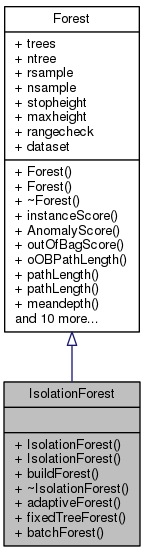
\includegraphics[width=180pt]{classIsolationForest__inherit__graph}
\end{center}
\end{figure}


Collaboration diagram for Isolation\+Forest\+:\nopagebreak
\begin{figure}[H]
\begin{center}
\leavevmode
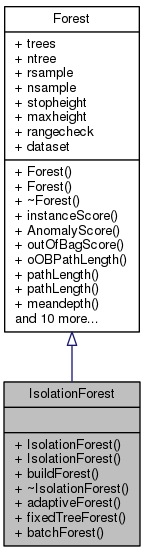
\includegraphics[width=180pt]{classIsolationForest__coll__graph}
\end{center}
\end{figure}
\subsection*{Public Member Functions}
\begin{DoxyCompactItemize}
\item 
\hyperlink{classIsolationForest_a381db4db6b4c0b3e532f67398b50e32a}{Isolation\+Forest} ()=default
\item 
\hyperlink{classIsolationForest_aa81cd568d5db199124cf381615cece42}{Isolation\+Forest} (int \+\_\+ntree, doubleframe $\ast$\+\_\+df, int \+\_\+nsample, int \+\_\+maxheight, bool \+\_\+stopheight, bool \+\_\+rsample)
\item 
void \hyperlink{classIsolationForest_a82005a7421ba74d37f7b5d24949c9e91}{build\+Forest} ()
\item 
virtual \hyperlink{classIsolationForest_add206f655ddfa46c359ae72ce4b5c66c}{$\sim$\+Isolation\+Forest} ()=default
\item 
int \hyperlink{classIsolationForest_a33dae487524bd1fdaf085a36dab04ee9}{adaptive\+Forest} (double alpha, int stop\+Limit)
\item 
void \hyperlink{classIsolationForest_a252267bf58f8bb812c4dca47d5390709}{fixed\+Tree\+Forest} (int epoch)
\item 
int \hyperlink{classIsolationForest_a10ab0476940aab9d6aa877d002fa9d5d}{batch\+Forest} (int epoch)
\end{DoxyCompactItemize}
\subsection*{Additional Inherited Members}


\subsection{Constructor \& Destructor Documentation}
\mbox{\Hypertarget{classIsolationForest_a381db4db6b4c0b3e532f67398b50e32a}\label{classIsolationForest_a381db4db6b4c0b3e532f67398b50e32a}} 
\index{Isolation\+Forest@{Isolation\+Forest}!Isolation\+Forest@{Isolation\+Forest}}
\index{Isolation\+Forest@{Isolation\+Forest}!Isolation\+Forest@{Isolation\+Forest}}
\subsubsection{\texorpdfstring{Isolation\+Forest()}{IsolationForest()}\hspace{0.1cm}{\footnotesize\ttfamily [1/2]}}
{\footnotesize\ttfamily Isolation\+Forest\+::\+Isolation\+Forest (\begin{DoxyParamCaption}{ }\end{DoxyParamCaption})\hspace{0.3cm}{\ttfamily [default]}}

\mbox{\Hypertarget{classIsolationForest_aa81cd568d5db199124cf381615cece42}\label{classIsolationForest_aa81cd568d5db199124cf381615cece42}} 
\index{Isolation\+Forest@{Isolation\+Forest}!Isolation\+Forest@{Isolation\+Forest}}
\index{Isolation\+Forest@{Isolation\+Forest}!Isolation\+Forest@{Isolation\+Forest}}
\subsubsection{\texorpdfstring{Isolation\+Forest()}{IsolationForest()}\hspace{0.1cm}{\footnotesize\ttfamily [2/2]}}
{\footnotesize\ttfamily Isolation\+Forest\+::\+Isolation\+Forest (\begin{DoxyParamCaption}\item[{int}]{\+\_\+ntree,  }\item[{doubleframe $\ast$}]{\+\_\+df,  }\item[{int}]{\+\_\+nsample,  }\item[{int}]{\+\_\+maxheight,  }\item[{bool}]{\+\_\+stopheight,  }\item[{bool}]{\+\_\+rsample }\end{DoxyParamCaption})}

\mbox{\Hypertarget{classIsolationForest_add206f655ddfa46c359ae72ce4b5c66c}\label{classIsolationForest_add206f655ddfa46c359ae72ce4b5c66c}} 
\index{Isolation\+Forest@{Isolation\+Forest}!````~Isolation\+Forest@{$\sim$\+Isolation\+Forest}}
\index{````~Isolation\+Forest@{$\sim$\+Isolation\+Forest}!Isolation\+Forest@{Isolation\+Forest}}
\subsubsection{\texorpdfstring{$\sim$\+Isolation\+Forest()}{~IsolationForest()}}
{\footnotesize\ttfamily virtual Isolation\+Forest\+::$\sim$\+Isolation\+Forest (\begin{DoxyParamCaption}{ }\end{DoxyParamCaption})\hspace{0.3cm}{\ttfamily [virtual]}, {\ttfamily [default]}}



\subsection{Member Function Documentation}
\mbox{\Hypertarget{classIsolationForest_a33dae487524bd1fdaf085a36dab04ee9}\label{classIsolationForest_a33dae487524bd1fdaf085a36dab04ee9}} 
\index{Isolation\+Forest@{Isolation\+Forest}!adaptive\+Forest@{adaptive\+Forest}}
\index{adaptive\+Forest@{adaptive\+Forest}!Isolation\+Forest@{Isolation\+Forest}}
\subsubsection{\texorpdfstring{adaptive\+Forest()}{adaptiveForest()}}
{\footnotesize\ttfamily int Isolation\+Forest\+::adaptive\+Forest (\begin{DoxyParamCaption}\item[{double}]{alpha,  }\item[{int}]{stop\+Limit }\end{DoxyParamCaption})\hspace{0.3cm}{\ttfamily [virtual]}}



Reimplemented from \hyperlink{classForest_a825bb350730c50aa8924e9f761c4a2a4}{Forest}.

\mbox{\Hypertarget{classIsolationForest_a10ab0476940aab9d6aa877d002fa9d5d}\label{classIsolationForest_a10ab0476940aab9d6aa877d002fa9d5d}} 
\index{Isolation\+Forest@{Isolation\+Forest}!batch\+Forest@{batch\+Forest}}
\index{batch\+Forest@{batch\+Forest}!Isolation\+Forest@{Isolation\+Forest}}
\subsubsection{\texorpdfstring{batch\+Forest()}{batchForest()}}
{\footnotesize\ttfamily int Isolation\+Forest\+::batch\+Forest (\begin{DoxyParamCaption}\item[{int}]{epoch }\end{DoxyParamCaption})}

\mbox{\Hypertarget{classIsolationForest_a82005a7421ba74d37f7b5d24949c9e91}\label{classIsolationForest_a82005a7421ba74d37f7b5d24949c9e91}} 
\index{Isolation\+Forest@{Isolation\+Forest}!build\+Forest@{build\+Forest}}
\index{build\+Forest@{build\+Forest}!Isolation\+Forest@{Isolation\+Forest}}
\subsubsection{\texorpdfstring{build\+Forest()}{buildForest()}}
{\footnotesize\ttfamily void Isolation\+Forest\+::build\+Forest (\begin{DoxyParamCaption}{ }\end{DoxyParamCaption})}

\mbox{\Hypertarget{classIsolationForest_a252267bf58f8bb812c4dca47d5390709}\label{classIsolationForest_a252267bf58f8bb812c4dca47d5390709}} 
\index{Isolation\+Forest@{Isolation\+Forest}!fixed\+Tree\+Forest@{fixed\+Tree\+Forest}}
\index{fixed\+Tree\+Forest@{fixed\+Tree\+Forest}!Isolation\+Forest@{Isolation\+Forest}}
\subsubsection{\texorpdfstring{fixed\+Tree\+Forest()}{fixedTreeForest()}}
{\footnotesize\ttfamily void Isolation\+Forest\+::fixed\+Tree\+Forest (\begin{DoxyParamCaption}\item[{int}]{epoch }\end{DoxyParamCaption})\hspace{0.3cm}{\ttfamily [virtual]}}



Reimplemented from \hyperlink{classForest_a0699073aa8d6b46fdbdc36b7299a1a34}{Forest}.



The documentation for this class was generated from the following files\+:\begin{DoxyCompactItemize}
\item 
src/\hyperlink{IsolationForest_8hpp}{Isolation\+Forest.\+hpp}\item 
src/\hyperlink{IsolationForest_8cpp}{Isolation\+Forest.\+cpp}\end{DoxyCompactItemize}

\hypertarget{structForest_1_1larger}{}\section{Forest\+:\+:larger Struct Reference}
\label{structForest_1_1larger}\index{Forest\+::larger@{Forest\+::larger}}


{\ttfamily \#include $<$Forest.\+hpp$>$}



Collaboration diagram for Forest\+:\+:larger\+:\nopagebreak
\begin{figure}[H]
\begin{center}
\leavevmode
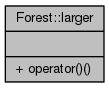
\includegraphics[width=154pt]{structForest_1_1larger__coll__graph}
\end{center}
\end{figure}
\subsection*{Public Member Functions}
\begin{DoxyCompactItemize}
\item 
bool \hyperlink{structForest_1_1larger_a9c11ad031d639515e945e085de4448a4}{operator()} (const std\+::pair$<$ int, double $>$ p1, const std\+::pair$<$ int, double $>$ p2)
\end{DoxyCompactItemize}


\subsection{Member Function Documentation}
\mbox{\Hypertarget{structForest_1_1larger_a9c11ad031d639515e945e085de4448a4}\label{structForest_1_1larger_a9c11ad031d639515e945e085de4448a4}} 
\index{Forest\+::larger@{Forest\+::larger}!operator()@{operator()}}
\index{operator()@{operator()}!Forest\+::larger@{Forest\+::larger}}
\subsubsection{\texorpdfstring{operator()()}{operator()()}}
{\footnotesize\ttfamily bool Forest\+::larger\+::operator() (\begin{DoxyParamCaption}\item[{const std\+::pair$<$ int, double $>$}]{p1,  }\item[{const std\+::pair$<$ int, double $>$}]{p2 }\end{DoxyParamCaption})\hspace{0.3cm}{\ttfamily [inline]}}



The documentation for this struct was generated from the following file\+:\begin{DoxyCompactItemize}
\item 
src/\hyperlink{Forest_8hpp}{Forest.\+hpp}\end{DoxyCompactItemize}

\hypertarget{structconvForest_1_1larger}{}\section{conv\+Forest\+:\+:larger Struct Reference}
\label{structconvForest_1_1larger}\index{conv\+Forest\+::larger@{conv\+Forest\+::larger}}


Collaboration diagram for conv\+Forest\+:\+:larger\+:\nopagebreak
\begin{figure}[H]
\begin{center}
\leavevmode
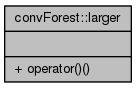
\includegraphics[width=174pt]{structconvForest_1_1larger__coll__graph}
\end{center}
\end{figure}
\subsection*{Public Member Functions}
\begin{DoxyCompactItemize}
\item 
bool \hyperlink{structconvForest_1_1larger_a1abbac0ea812a054a6572dd5046a9901}{operator()} (const std\+::pair$<$ int, double $>$ p1, const std\+::pair$<$ int, double $>$ p2)
\end{DoxyCompactItemize}


\subsection{Member Function Documentation}
\mbox{\Hypertarget{structconvForest_1_1larger_a1abbac0ea812a054a6572dd5046a9901}\label{structconvForest_1_1larger_a1abbac0ea812a054a6572dd5046a9901}} 
\index{conv\+Forest\+::larger@{conv\+Forest\+::larger}!operator()@{operator()}}
\index{operator()@{operator()}!conv\+Forest\+::larger@{conv\+Forest\+::larger}}
\subsubsection{\texorpdfstring{operator()()}{operator()()}}
{\footnotesize\ttfamily bool conv\+Forest\+::larger\+::operator() (\begin{DoxyParamCaption}\item[{const std\+::pair$<$ int, double $>$}]{p1,  }\item[{const std\+::pair$<$ int, double $>$}]{p2 }\end{DoxyParamCaption})\hspace{0.3cm}{\ttfamily [inline]}}



The documentation for this struct was generated from the following file\+:\begin{DoxyCompactItemize}
\item 
src/\hyperlink{convForest_8hpp}{conv\+Forest.\+hpp}\end{DoxyCompactItemize}

\hypertarget{classutil_1_1Matrix}{}\section{util\+:\+:Matrix$<$ T $>$ Class Template Reference}
\label{classutil_1_1Matrix}\index{util\+::\+Matrix$<$ T $>$@{util\+::\+Matrix$<$ T $>$}}


{\ttfamily \#include $<$utility.\+hpp$>$}



Collaboration diagram for util\+:\+:Matrix$<$ T $>$\+:\nopagebreak
\begin{figure}[H]
\begin{center}
\leavevmode
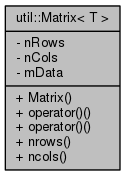
\includegraphics[width=166pt]{classutil_1_1Matrix__coll__graph}
\end{center}
\end{figure}
\subsection*{Public Member Functions}
\begin{DoxyCompactItemize}
\item 
\hyperlink{classutil_1_1Matrix_aa68ae4682b48d4f40bc2a3ef0ed75976}{Matrix} (size\+\_\+t rows, size\+\_\+t cols)
\item 
double \& \hyperlink{classutil_1_1Matrix_a7c2d260e685310c403600ed18f02f967}{operator()} (size\+\_\+t i, size\+\_\+t j)
\item 
double \hyperlink{classutil_1_1Matrix_a1cdfea411728de3e4028d44cfbb4b54a}{operator()} (size\+\_\+t i, size\+\_\+t j) const
\item 
int \hyperlink{classutil_1_1Matrix_a58f84228a561ec5152e8fd9d3800e7bc}{nrows} ()
\item 
size\+\_\+t \hyperlink{classutil_1_1Matrix_a728bc44831ab516e0a46c1c342e8b996}{ncols} ()
\end{DoxyCompactItemize}
\subsection*{Private Attributes}
\begin{DoxyCompactItemize}
\item 
size\+\_\+t \hyperlink{classutil_1_1Matrix_a1d981a6aa70209f8cf1e3fb7a0820240}{n\+Rows}
\item 
size\+\_\+t \hyperlink{classutil_1_1Matrix_ae93dd1e2ede96c42b2035a69e4a14083}{n\+Cols}
\item 
std\+::vector$<$ T $>$ \hyperlink{classutil_1_1Matrix_ad8ef42880d189249c526aca3825be2cf}{m\+Data}
\end{DoxyCompactItemize}


\subsection{Constructor \& Destructor Documentation}
\mbox{\Hypertarget{classutil_1_1Matrix_aa68ae4682b48d4f40bc2a3ef0ed75976}\label{classutil_1_1Matrix_aa68ae4682b48d4f40bc2a3ef0ed75976}} 
\index{util\+::\+Matrix@{util\+::\+Matrix}!Matrix@{Matrix}}
\index{Matrix@{Matrix}!util\+::\+Matrix@{util\+::\+Matrix}}
\subsubsection{\texorpdfstring{Matrix()}{Matrix()}}
{\footnotesize\ttfamily template$<$typename T $>$ \\
\hyperlink{classutil_1_1Matrix}{util\+::\+Matrix}$<$ T $>$\+::\hyperlink{classutil_1_1Matrix}{Matrix} (\begin{DoxyParamCaption}\item[{size\+\_\+t}]{rows,  }\item[{size\+\_\+t}]{cols }\end{DoxyParamCaption})}

\hyperlink{classutil_1_1Matrix}{Matrix} class


\begin{DoxyParams}{Parameters}
{\em D} & \\
\hline
{\em N} & \\
\hline
\end{DoxyParams}
\begin{DoxyReturn}{Returns}

\end{DoxyReturn}


\subsection{Member Function Documentation}
\mbox{\Hypertarget{classutil_1_1Matrix_a728bc44831ab516e0a46c1c342e8b996}\label{classutil_1_1Matrix_a728bc44831ab516e0a46c1c342e8b996}} 
\index{util\+::\+Matrix@{util\+::\+Matrix}!ncols@{ncols}}
\index{ncols@{ncols}!util\+::\+Matrix@{util\+::\+Matrix}}
\subsubsection{\texorpdfstring{ncols()}{ncols()}}
{\footnotesize\ttfamily template$<$typename T$>$ \\
size\+\_\+t \hyperlink{classutil_1_1Matrix}{util\+::\+Matrix}$<$ T $>$\+::ncols (\begin{DoxyParamCaption}{ }\end{DoxyParamCaption})}

\mbox{\Hypertarget{classutil_1_1Matrix_a58f84228a561ec5152e8fd9d3800e7bc}\label{classutil_1_1Matrix_a58f84228a561ec5152e8fd9d3800e7bc}} 
\index{util\+::\+Matrix@{util\+::\+Matrix}!nrows@{nrows}}
\index{nrows@{nrows}!util\+::\+Matrix@{util\+::\+Matrix}}
\subsubsection{\texorpdfstring{nrows()}{nrows()}}
{\footnotesize\ttfamily template$<$typename T$>$ \\
int \hyperlink{classutil_1_1Matrix}{util\+::\+Matrix}$<$ T $>$\+::nrows (\begin{DoxyParamCaption}{ }\end{DoxyParamCaption})}

\mbox{\Hypertarget{classutil_1_1Matrix_a7c2d260e685310c403600ed18f02f967}\label{classutil_1_1Matrix_a7c2d260e685310c403600ed18f02f967}} 
\index{util\+::\+Matrix@{util\+::\+Matrix}!operator()@{operator()}}
\index{operator()@{operator()}!util\+::\+Matrix@{util\+::\+Matrix}}
\subsubsection{\texorpdfstring{operator()()}{operator()()}\hspace{0.1cm}{\footnotesize\ttfamily [1/2]}}
{\footnotesize\ttfamily template$<$typename T $>$ \\
double \& \hyperlink{classutil_1_1Matrix}{util\+::\+Matrix}$<$ T $>$\+::operator() (\begin{DoxyParamCaption}\item[{size\+\_\+t}]{i,  }\item[{size\+\_\+t}]{j }\end{DoxyParamCaption})}

\mbox{\Hypertarget{classutil_1_1Matrix_a1cdfea411728de3e4028d44cfbb4b54a}\label{classutil_1_1Matrix_a1cdfea411728de3e4028d44cfbb4b54a}} 
\index{util\+::\+Matrix@{util\+::\+Matrix}!operator()@{operator()}}
\index{operator()@{operator()}!util\+::\+Matrix@{util\+::\+Matrix}}
\subsubsection{\texorpdfstring{operator()()}{operator()()}\hspace{0.1cm}{\footnotesize\ttfamily [2/2]}}
{\footnotesize\ttfamily template$<$typename T $>$ \\
double \hyperlink{classutil_1_1Matrix}{util\+::\+Matrix}$<$ T $>$\+::operator() (\begin{DoxyParamCaption}\item[{size\+\_\+t}]{i,  }\item[{size\+\_\+t}]{j }\end{DoxyParamCaption}) const}



\subsection{Field Documentation}
\mbox{\Hypertarget{classutil_1_1Matrix_ad8ef42880d189249c526aca3825be2cf}\label{classutil_1_1Matrix_ad8ef42880d189249c526aca3825be2cf}} 
\index{util\+::\+Matrix@{util\+::\+Matrix}!m\+Data@{m\+Data}}
\index{m\+Data@{m\+Data}!util\+::\+Matrix@{util\+::\+Matrix}}
\subsubsection{\texorpdfstring{m\+Data}{mData}}
{\footnotesize\ttfamily template$<$typename T$>$ \\
std\+::vector$<$T$>$ \hyperlink{classutil_1_1Matrix}{util\+::\+Matrix}$<$ T $>$\+::m\+Data\hspace{0.3cm}{\ttfamily [private]}}

\mbox{\Hypertarget{classutil_1_1Matrix_ae93dd1e2ede96c42b2035a69e4a14083}\label{classutil_1_1Matrix_ae93dd1e2ede96c42b2035a69e4a14083}} 
\index{util\+::\+Matrix@{util\+::\+Matrix}!n\+Cols@{n\+Cols}}
\index{n\+Cols@{n\+Cols}!util\+::\+Matrix@{util\+::\+Matrix}}
\subsubsection{\texorpdfstring{n\+Cols}{nCols}}
{\footnotesize\ttfamily template$<$typename T$>$ \\
size\+\_\+t \hyperlink{classutil_1_1Matrix}{util\+::\+Matrix}$<$ T $>$\+::n\+Cols\hspace{0.3cm}{\ttfamily [private]}}

\mbox{\Hypertarget{classutil_1_1Matrix_a1d981a6aa70209f8cf1e3fb7a0820240}\label{classutil_1_1Matrix_a1d981a6aa70209f8cf1e3fb7a0820240}} 
\index{util\+::\+Matrix@{util\+::\+Matrix}!n\+Rows@{n\+Rows}}
\index{n\+Rows@{n\+Rows}!util\+::\+Matrix@{util\+::\+Matrix}}
\subsubsection{\texorpdfstring{n\+Rows}{nRows}}
{\footnotesize\ttfamily template$<$typename T$>$ \\
size\+\_\+t \hyperlink{classutil_1_1Matrix}{util\+::\+Matrix}$<$ T $>$\+::n\+Rows\hspace{0.3cm}{\ttfamily [private]}}



The documentation for this class was generated from the following files\+:\begin{DoxyCompactItemize}
\item 
src/\hyperlink{utility_8hpp}{utility.\+hpp}\item 
src/\hyperlink{utility_8cpp}{utility.\+cpp}\end{DoxyCompactItemize}

\hypertarget{structOOBEstimator}{}\section{O\+O\+B\+Estimator Struct Reference}
\label{structOOBEstimator}\index{O\+O\+B\+Estimator@{O\+O\+B\+Estimator}}


{\ttfamily \#include $<$O\+O\+B\+Estimator.\+hpp$>$}



Collaboration diagram for O\+O\+B\+Estimator\+:\nopagebreak
\begin{figure}[H]
\begin{center}
\leavevmode
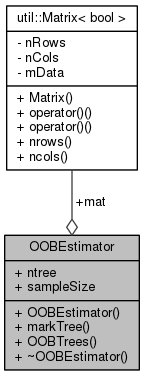
\includegraphics[width=180pt]{structOOBEstimator__coll__graph}
\end{center}
\end{figure}
\subsection*{Public Member Functions}
\begin{DoxyCompactItemize}
\item 
\hyperlink{structOOBEstimator_a14346003c044f4f83d901191db629838}{O\+O\+B\+Estimator} (size\+\_\+t \+\_\+ntree, size\+\_\+t \+\_\+nsample)
\item 
void \hyperlink{structOOBEstimator_a3f6c58438a669a75c2013e284c16c038}{mark\+Tree} (int tree\+Index, int x\+Index)
\item 
std\+::vector$<$ int $>$ \hyperlink{structOOBEstimator_a562eaa254b4d88129369ca3a33cd03f2}{O\+O\+B\+Trees} (int x\+Index)
\item 
\hyperlink{structOOBEstimator_a52be024d6b911e15a162f92c44760b7d}{$\sim$\+O\+O\+B\+Estimator} ()
\end{DoxyCompactItemize}
\subsection*{Data Fields}
\begin{DoxyCompactItemize}
\item 
\hyperlink{classutil_1_1Matrix}{util\+::\+Matrix}$<$ bool $>$ $\ast$ \hyperlink{structOOBEstimator_adff3279f68eba078d403e2673aa6627e}{mat}
\item 
int \hyperlink{structOOBEstimator_af09c508b17686ca379d67affa1f31333}{ntree}
\item 
int \hyperlink{structOOBEstimator_a199a3bf3234bd967e061b1c61a56aed6}{sample\+Size}
\end{DoxyCompactItemize}


\subsection{Constructor \& Destructor Documentation}
\mbox{\Hypertarget{structOOBEstimator_a14346003c044f4f83d901191db629838}\label{structOOBEstimator_a14346003c044f4f83d901191db629838}} 
\index{O\+O\+B\+Estimator@{O\+O\+B\+Estimator}!O\+O\+B\+Estimator@{O\+O\+B\+Estimator}}
\index{O\+O\+B\+Estimator@{O\+O\+B\+Estimator}!O\+O\+B\+Estimator@{O\+O\+B\+Estimator}}
\subsubsection{\texorpdfstring{O\+O\+B\+Estimator()}{OOBEstimator()}}
{\footnotesize\ttfamily O\+O\+B\+Estimator\+::\+O\+O\+B\+Estimator (\begin{DoxyParamCaption}\item[{size\+\_\+t}]{\+\_\+ntree,  }\item[{size\+\_\+t}]{\+\_\+nsample }\end{DoxyParamCaption})\hspace{0.3cm}{\ttfamily [inline]}}

\mbox{\Hypertarget{structOOBEstimator_a52be024d6b911e15a162f92c44760b7d}\label{structOOBEstimator_a52be024d6b911e15a162f92c44760b7d}} 
\index{O\+O\+B\+Estimator@{O\+O\+B\+Estimator}!````~O\+O\+B\+Estimator@{$\sim$\+O\+O\+B\+Estimator}}
\index{````~O\+O\+B\+Estimator@{$\sim$\+O\+O\+B\+Estimator}!O\+O\+B\+Estimator@{O\+O\+B\+Estimator}}
\subsubsection{\texorpdfstring{$\sim$\+O\+O\+B\+Estimator()}{~OOBEstimator()}}
{\footnotesize\ttfamily O\+O\+B\+Estimator\+::$\sim$\+O\+O\+B\+Estimator (\begin{DoxyParamCaption}{ }\end{DoxyParamCaption})\hspace{0.3cm}{\ttfamily [inline]}}



\subsection{Member Function Documentation}
\mbox{\Hypertarget{structOOBEstimator_a3f6c58438a669a75c2013e284c16c038}\label{structOOBEstimator_a3f6c58438a669a75c2013e284c16c038}} 
\index{O\+O\+B\+Estimator@{O\+O\+B\+Estimator}!mark\+Tree@{mark\+Tree}}
\index{mark\+Tree@{mark\+Tree}!O\+O\+B\+Estimator@{O\+O\+B\+Estimator}}
\subsubsection{\texorpdfstring{mark\+Tree()}{markTree()}}
{\footnotesize\ttfamily void O\+O\+B\+Estimator\+::mark\+Tree (\begin{DoxyParamCaption}\item[{int}]{tree\+Index,  }\item[{int}]{x\+Index }\end{DoxyParamCaption})\hspace{0.3cm}{\ttfamily [inline]}}

\mbox{\Hypertarget{structOOBEstimator_a562eaa254b4d88129369ca3a33cd03f2}\label{structOOBEstimator_a562eaa254b4d88129369ca3a33cd03f2}} 
\index{O\+O\+B\+Estimator@{O\+O\+B\+Estimator}!O\+O\+B\+Trees@{O\+O\+B\+Trees}}
\index{O\+O\+B\+Trees@{O\+O\+B\+Trees}!O\+O\+B\+Estimator@{O\+O\+B\+Estimator}}
\subsubsection{\texorpdfstring{O\+O\+B\+Trees()}{OOBTrees()}}
{\footnotesize\ttfamily std\+::vector$<$int$>$ O\+O\+B\+Estimator\+::\+O\+O\+B\+Trees (\begin{DoxyParamCaption}\item[{int}]{x\+Index }\end{DoxyParamCaption})\hspace{0.3cm}{\ttfamily [inline]}}

Returns all out of bag trees that don\textquotesingle{}t invole x 
\begin{DoxyParams}{Parameters}
{\em x\+Index} & \+: int index of sample \\
\hline
\end{DoxyParams}
\begin{DoxyReturn}{Returns}
\hyperlink{classTree}{Tree} index in the forest that X\+Index don\textquotesingle{}t involve 
\end{DoxyReturn}


\subsection{Field Documentation}
\mbox{\Hypertarget{structOOBEstimator_adff3279f68eba078d403e2673aa6627e}\label{structOOBEstimator_adff3279f68eba078d403e2673aa6627e}} 
\index{O\+O\+B\+Estimator@{O\+O\+B\+Estimator}!mat@{mat}}
\index{mat@{mat}!O\+O\+B\+Estimator@{O\+O\+B\+Estimator}}
\subsubsection{\texorpdfstring{mat}{mat}}
{\footnotesize\ttfamily \hyperlink{classutil_1_1Matrix}{util\+::\+Matrix}$<$bool$>$$\ast$ O\+O\+B\+Estimator\+::mat}

\mbox{\Hypertarget{structOOBEstimator_af09c508b17686ca379d67affa1f31333}\label{structOOBEstimator_af09c508b17686ca379d67affa1f31333}} 
\index{O\+O\+B\+Estimator@{O\+O\+B\+Estimator}!ntree@{ntree}}
\index{ntree@{ntree}!O\+O\+B\+Estimator@{O\+O\+B\+Estimator}}
\subsubsection{\texorpdfstring{ntree}{ntree}}
{\footnotesize\ttfamily int O\+O\+B\+Estimator\+::ntree}

\mbox{\Hypertarget{structOOBEstimator_a199a3bf3234bd967e061b1c61a56aed6}\label{structOOBEstimator_a199a3bf3234bd967e061b1c61a56aed6}} 
\index{O\+O\+B\+Estimator@{O\+O\+B\+Estimator}!sample\+Size@{sample\+Size}}
\index{sample\+Size@{sample\+Size}!O\+O\+B\+Estimator@{O\+O\+B\+Estimator}}
\subsubsection{\texorpdfstring{sample\+Size}{sampleSize}}
{\footnotesize\ttfamily int O\+O\+B\+Estimator\+::sample\+Size}



The documentation for this struct was generated from the following file\+:\begin{DoxyCompactItemize}
\item 
src/\hyperlink{OOBEstimator_8hpp}{O\+O\+B\+Estimator.\+hpp}\end{DoxyCompactItemize}

\hypertarget{classRForest}{}\section{R\+Forest Class Reference}
\label{classRForest}\index{R\+Forest@{R\+Forest}}


{\ttfamily \#include $<$R\+Forest.\+hpp$>$}



Inheritance diagram for R\+Forest\+:\nopagebreak
\begin{figure}[H]
\begin{center}
\leavevmode
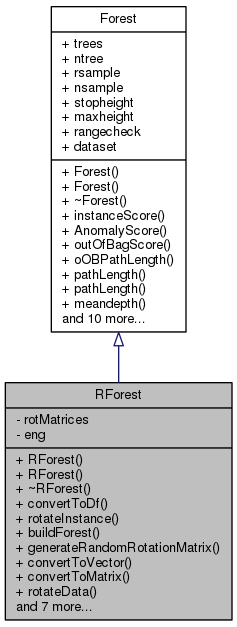
\includegraphics[width=250pt]{classRForest__inherit__graph}
\end{center}
\end{figure}


Collaboration diagram for R\+Forest\+:\nopagebreak
\begin{figure}[H]
\begin{center}
\leavevmode
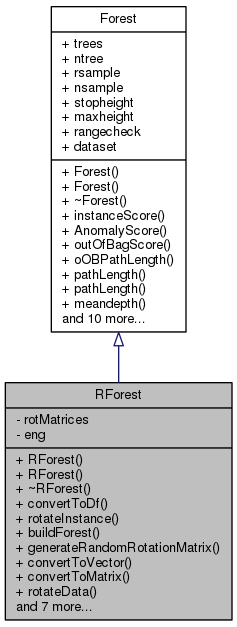
\includegraphics[width=250pt]{classRForest__coll__graph}
\end{center}
\end{figure}
\subsection*{Public Member Functions}
\begin{DoxyCompactItemize}
\item 
\hyperlink{classRForest_a3314b007aa19d928f56f4bbaf35fae10}{R\+Forest} (int \+\_\+ntree, doubleframe $\ast$\+\_\+df, int \+\_\+nsample, int \+\_\+maxheight, bool \+\_\+stopheight, bool \+\_\+rsample)
\item 
\hyperlink{classRForest_a6058c1b7beb5c90e59e558847b8650f6}{R\+Forest} ()
\item 
\hyperlink{classRForest_a873a1b941163b4cccda4bf83607226f3}{$\sim$\+R\+Forest} ()
\item 
void \hyperlink{classRForest_a0d8c5dbc04ec8433403f40d289d28100}{convert\+To\+Df} (Eigen\+::\+Matrix\+Xd \&m, doubleframe $\ast$df)
\item 
void \hyperlink{classRForest_a068f39ee76aa3ece35f110975303f07b}{rotate\+Instance} (double $\ast$inst, Eigen\+::\+Matrix\+Xd \&m, double $\ast$rotated\+Data)
\item 
void \hyperlink{classRForest_a7e8959b5b54b454f34ed68d60132e80f}{build\+Forest} (doubleframe $\ast$df)
\item 
void \hyperlink{classRForest_ab1f0edda495b87ef9286907d44f2f8ff}{generate\+Random\+Rotation\+Matrix} (Eigen\+::\+Matrix\+Xd \&M, int n)
\item 
void \hyperlink{classRForest_ada11eb452d05c98cd481b9080a5703a3}{convert\+To\+Vector} (Eigen\+::\+Matrix\+Xd \&m, std\+::vector$<$ std\+::vector$<$ double $>$ $>$ \&v)
\item 
Eigen\+::\+Matrix\+Xd \hyperlink{classRForest_ad132bc186056d96d8979fbe238afe529}{convert\+To\+Matrix} (std\+::vector$<$ std\+::vector$<$ double $>$ $>$ \&data)
\item 
Eigen\+::\+Matrix\+Xd \hyperlink{classRForest_af149cda8d70a254ff0968d350f85b59d}{rotate\+Data} (doubleframe $\ast$dt, Eigen\+::\+Matrix\+Xd \&M)
\item 
Eigen\+::\+Matrix\+Xd \hyperlink{classRForest_a17f0ad7b46a5bceff43411d4752002d3}{convert\+Df\+To\+Matrix} (const doubleframe $\ast$data, std\+::vector$<$ int $>$ \&sample\+Index)
\item 
std\+::vector$<$ double $>$ \hyperlink{classRForest_ad2631b9a85a04079c603b1c8296bdb9d}{path\+Length} (double $\ast$inst)
\item 
double \hyperlink{classRForest_a3ecb236540eade88548b9e7ace6f13a1}{getdepth} (double $\ast$inst, std\+::shared\+\_\+ptr$<$ \hyperlink{classTree}{Tree} $>$ tree, Eigen\+::\+Matrix\+Xd \&rotmat, double $\ast$trans\+Inst)
\item 
void \hyperlink{classRForest_af91b647289cd5631389cefbc2612f4b3}{r\+Forest} ()
\item 
int \hyperlink{classRForest_abc389cab7fa7ffee669b3add5aad4c52}{adaptive\+Forest} (double alpha, int stop\+Limit)
\item 
void \hyperlink{classRForest_af8c8c06e5875c4a2a539d38ec65c9a7e}{fixed\+Tree\+Forest} (int epoch)
\item 
void \hyperlink{classRForest_ab6d2b335db34e4845bebf8864cc4e0e1}{projected\+Forest} ()
\end{DoxyCompactItemize}
\subsection*{Private Attributes}
\begin{DoxyCompactItemize}
\item 
std\+::vector$<$ Eigen\+::\+Matrix\+Xd $>$ \hyperlink{classRForest_a2b03a249697e9a68362455a6be8b1762}{rot\+Matrices}
\item 
std\+::mt19937 \hyperlink{classRForest_ae42cae6b10ed270d226dc2871a1b4c5a}{eng} \{std\+::random\+\_\+device\{\}()\}
\end{DoxyCompactItemize}
\subsection*{Additional Inherited Members}


\subsection{Constructor \& Destructor Documentation}
\mbox{\Hypertarget{classRForest_a3314b007aa19d928f56f4bbaf35fae10}\label{classRForest_a3314b007aa19d928f56f4bbaf35fae10}} 
\index{R\+Forest@{R\+Forest}!R\+Forest@{R\+Forest}}
\index{R\+Forest@{R\+Forest}!R\+Forest@{R\+Forest}}
\subsubsection{\texorpdfstring{R\+Forest()}{RForest()}\hspace{0.1cm}{\footnotesize\ttfamily [1/2]}}
{\footnotesize\ttfamily R\+Forest\+::\+R\+Forest (\begin{DoxyParamCaption}\item[{int}]{\+\_\+ntree,  }\item[{doubleframe $\ast$}]{\+\_\+df,  }\item[{int}]{\+\_\+nsample,  }\item[{int}]{\+\_\+maxheight,  }\item[{bool}]{\+\_\+stopheight,  }\item[{bool}]{\+\_\+rsample }\end{DoxyParamCaption})\hspace{0.3cm}{\ttfamily [inline]}}

\mbox{\Hypertarget{classRForest_a6058c1b7beb5c90e59e558847b8650f6}\label{classRForest_a6058c1b7beb5c90e59e558847b8650f6}} 
\index{R\+Forest@{R\+Forest}!R\+Forest@{R\+Forest}}
\index{R\+Forest@{R\+Forest}!R\+Forest@{R\+Forest}}
\subsubsection{\texorpdfstring{R\+Forest()}{RForest()}\hspace{0.1cm}{\footnotesize\ttfamily [2/2]}}
{\footnotesize\ttfamily R\+Forest\+::\+R\+Forest (\begin{DoxyParamCaption}{ }\end{DoxyParamCaption})\hspace{0.3cm}{\ttfamily [inline]}}

\mbox{\Hypertarget{classRForest_a873a1b941163b4cccda4bf83607226f3}\label{classRForest_a873a1b941163b4cccda4bf83607226f3}} 
\index{R\+Forest@{R\+Forest}!````~R\+Forest@{$\sim$\+R\+Forest}}
\index{````~R\+Forest@{$\sim$\+R\+Forest}!R\+Forest@{R\+Forest}}
\subsubsection{\texorpdfstring{$\sim$\+R\+Forest()}{~RForest()}}
{\footnotesize\ttfamily R\+Forest\+::$\sim$\+R\+Forest (\begin{DoxyParamCaption}{ }\end{DoxyParamCaption})\hspace{0.3cm}{\ttfamily [inline]}}



\subsection{Member Function Documentation}
\mbox{\Hypertarget{classRForest_abc389cab7fa7ffee669b3add5aad4c52}\label{classRForest_abc389cab7fa7ffee669b3add5aad4c52}} 
\index{R\+Forest@{R\+Forest}!adaptive\+Forest@{adaptive\+Forest}}
\index{adaptive\+Forest@{adaptive\+Forest}!R\+Forest@{R\+Forest}}
\subsubsection{\texorpdfstring{adaptive\+Forest()}{adaptiveForest()}}
{\footnotesize\ttfamily int R\+Forest\+::adaptive\+Forest (\begin{DoxyParamCaption}\item[{double}]{alpha,  }\item[{int}]{stop\+Limit }\end{DoxyParamCaption})\hspace{0.3cm}{\ttfamily [virtual]}}



Reimplemented from \hyperlink{classForest_a825bb350730c50aa8924e9f761c4a2a4}{Forest}.

\mbox{\Hypertarget{classRForest_a7e8959b5b54b454f34ed68d60132e80f}\label{classRForest_a7e8959b5b54b454f34ed68d60132e80f}} 
\index{R\+Forest@{R\+Forest}!build\+Forest@{build\+Forest}}
\index{build\+Forest@{build\+Forest}!R\+Forest@{R\+Forest}}
\subsubsection{\texorpdfstring{build\+Forest()}{buildForest()}}
{\footnotesize\ttfamily void R\+Forest\+::build\+Forest (\begin{DoxyParamCaption}\item[{doubleframe $\ast$}]{df }\end{DoxyParamCaption})}

\mbox{\Hypertarget{classRForest_a17f0ad7b46a5bceff43411d4752002d3}\label{classRForest_a17f0ad7b46a5bceff43411d4752002d3}} 
\index{R\+Forest@{R\+Forest}!convert\+Df\+To\+Matrix@{convert\+Df\+To\+Matrix}}
\index{convert\+Df\+To\+Matrix@{convert\+Df\+To\+Matrix}!R\+Forest@{R\+Forest}}
\subsubsection{\texorpdfstring{convert\+Df\+To\+Matrix()}{convertDfToMatrix()}}
{\footnotesize\ttfamily Matrix\+Xd R\+Forest\+::convert\+Df\+To\+Matrix (\begin{DoxyParamCaption}\item[{const doubleframe $\ast$}]{data,  }\item[{std\+::vector$<$ int $>$ \&}]{sample\+Index }\end{DoxyParamCaption})}

\mbox{\Hypertarget{classRForest_a0d8c5dbc04ec8433403f40d289d28100}\label{classRForest_a0d8c5dbc04ec8433403f40d289d28100}} 
\index{R\+Forest@{R\+Forest}!convert\+To\+Df@{convert\+To\+Df}}
\index{convert\+To\+Df@{convert\+To\+Df}!R\+Forest@{R\+Forest}}
\subsubsection{\texorpdfstring{convert\+To\+Df()}{convertToDf()}}
{\footnotesize\ttfamily void R\+Forest\+::convert\+To\+Df (\begin{DoxyParamCaption}\item[{Eigen\+::\+Matrix\+Xd \&}]{m,  }\item[{doubleframe $\ast$}]{df }\end{DoxyParamCaption})}

\mbox{\Hypertarget{classRForest_ad132bc186056d96d8979fbe238afe529}\label{classRForest_ad132bc186056d96d8979fbe238afe529}} 
\index{R\+Forest@{R\+Forest}!convert\+To\+Matrix@{convert\+To\+Matrix}}
\index{convert\+To\+Matrix@{convert\+To\+Matrix}!R\+Forest@{R\+Forest}}
\subsubsection{\texorpdfstring{convert\+To\+Matrix()}{convertToMatrix()}}
{\footnotesize\ttfamily Matrix\+Xd R\+Forest\+::convert\+To\+Matrix (\begin{DoxyParamCaption}\item[{std\+::vector$<$ std\+::vector$<$ double $>$ $>$ \&}]{data }\end{DoxyParamCaption})}

\mbox{\Hypertarget{classRForest_ada11eb452d05c98cd481b9080a5703a3}\label{classRForest_ada11eb452d05c98cd481b9080a5703a3}} 
\index{R\+Forest@{R\+Forest}!convert\+To\+Vector@{convert\+To\+Vector}}
\index{convert\+To\+Vector@{convert\+To\+Vector}!R\+Forest@{R\+Forest}}
\subsubsection{\texorpdfstring{convert\+To\+Vector()}{convertToVector()}}
{\footnotesize\ttfamily void R\+Forest\+::convert\+To\+Vector (\begin{DoxyParamCaption}\item[{Eigen\+::\+Matrix\+Xd \&}]{m,  }\item[{std\+::vector$<$ std\+::vector$<$ double $>$ $>$ \&}]{v }\end{DoxyParamCaption})}

\mbox{\Hypertarget{classRForest_af8c8c06e5875c4a2a539d38ec65c9a7e}\label{classRForest_af8c8c06e5875c4a2a539d38ec65c9a7e}} 
\index{R\+Forest@{R\+Forest}!fixed\+Tree\+Forest@{fixed\+Tree\+Forest}}
\index{fixed\+Tree\+Forest@{fixed\+Tree\+Forest}!R\+Forest@{R\+Forest}}
\subsubsection{\texorpdfstring{fixed\+Tree\+Forest()}{fixedTreeForest()}}
{\footnotesize\ttfamily void R\+Forest\+::fixed\+Tree\+Forest (\begin{DoxyParamCaption}\item[{int}]{epoch }\end{DoxyParamCaption})\hspace{0.3cm}{\ttfamily [virtual]}}



Reimplemented from \hyperlink{classForest_a0699073aa8d6b46fdbdc36b7299a1a34}{Forest}.

\mbox{\Hypertarget{classRForest_ab1f0edda495b87ef9286907d44f2f8ff}\label{classRForest_ab1f0edda495b87ef9286907d44f2f8ff}} 
\index{R\+Forest@{R\+Forest}!generate\+Random\+Rotation\+Matrix@{generate\+Random\+Rotation\+Matrix}}
\index{generate\+Random\+Rotation\+Matrix@{generate\+Random\+Rotation\+Matrix}!R\+Forest@{R\+Forest}}
\subsubsection{\texorpdfstring{generate\+Random\+Rotation\+Matrix()}{generateRandomRotationMatrix()}}
{\footnotesize\ttfamily void R\+Forest\+::generate\+Random\+Rotation\+Matrix (\begin{DoxyParamCaption}\item[{Eigen\+::\+Matrix\+Xd \&}]{M,  }\item[{int}]{n }\end{DoxyParamCaption})}

\mbox{\Hypertarget{classRForest_a3ecb236540eade88548b9e7ace6f13a1}\label{classRForest_a3ecb236540eade88548b9e7ace6f13a1}} 
\index{R\+Forest@{R\+Forest}!getdepth@{getdepth}}
\index{getdepth@{getdepth}!R\+Forest@{R\+Forest}}
\subsubsection{\texorpdfstring{getdepth()}{getdepth()}}
{\footnotesize\ttfamily double R\+Forest\+::getdepth (\begin{DoxyParamCaption}\item[{double $\ast$}]{inst,  }\item[{std\+::shared\+\_\+ptr$<$ \hyperlink{classTree}{Tree} $>$}]{tree,  }\item[{Eigen\+::\+Matrix\+Xd \&}]{rotmat,  }\item[{double $\ast$}]{trans\+Inst }\end{DoxyParamCaption})}

\mbox{\Hypertarget{classRForest_ad2631b9a85a04079c603b1c8296bdb9d}\label{classRForest_ad2631b9a85a04079c603b1c8296bdb9d}} 
\index{R\+Forest@{R\+Forest}!path\+Length@{path\+Length}}
\index{path\+Length@{path\+Length}!R\+Forest@{R\+Forest}}
\subsubsection{\texorpdfstring{path\+Length()}{pathLength()}}
{\footnotesize\ttfamily std\+::vector$<$ double $>$ R\+Forest\+::path\+Length (\begin{DoxyParamCaption}\item[{double $\ast$}]{inst }\end{DoxyParamCaption})\hspace{0.3cm}{\ttfamily [virtual]}}



Reimplemented from \hyperlink{classForest_a8e3bac70e9f10ce6f301e297e32e8f5a}{Forest}.

\mbox{\Hypertarget{classRForest_ab6d2b335db34e4845bebf8864cc4e0e1}\label{classRForest_ab6d2b335db34e4845bebf8864cc4e0e1}} 
\index{R\+Forest@{R\+Forest}!projected\+Forest@{projected\+Forest}}
\index{projected\+Forest@{projected\+Forest}!R\+Forest@{R\+Forest}}
\subsubsection{\texorpdfstring{projected\+Forest()}{projectedForest()}}
{\footnotesize\ttfamily void R\+Forest\+::projected\+Forest (\begin{DoxyParamCaption}{ }\end{DoxyParamCaption})}

\mbox{\Hypertarget{classRForest_af91b647289cd5631389cefbc2612f4b3}\label{classRForest_af91b647289cd5631389cefbc2612f4b3}} 
\index{R\+Forest@{R\+Forest}!r\+Forest@{r\+Forest}}
\index{r\+Forest@{r\+Forest}!R\+Forest@{R\+Forest}}
\subsubsection{\texorpdfstring{r\+Forest()}{rForest()}}
{\footnotesize\ttfamily void R\+Forest\+::r\+Forest (\begin{DoxyParamCaption}{ }\end{DoxyParamCaption})}

\mbox{\Hypertarget{classRForest_af149cda8d70a254ff0968d350f85b59d}\label{classRForest_af149cda8d70a254ff0968d350f85b59d}} 
\index{R\+Forest@{R\+Forest}!rotate\+Data@{rotate\+Data}}
\index{rotate\+Data@{rotate\+Data}!R\+Forest@{R\+Forest}}
\subsubsection{\texorpdfstring{rotate\+Data()}{rotateData()}}
{\footnotesize\ttfamily Matrix\+Xd R\+Forest\+::rotate\+Data (\begin{DoxyParamCaption}\item[{doubleframe $\ast$}]{dt,  }\item[{Eigen\+::\+Matrix\+Xd \&}]{M }\end{DoxyParamCaption})}

\mbox{\Hypertarget{classRForest_a068f39ee76aa3ece35f110975303f07b}\label{classRForest_a068f39ee76aa3ece35f110975303f07b}} 
\index{R\+Forest@{R\+Forest}!rotate\+Instance@{rotate\+Instance}}
\index{rotate\+Instance@{rotate\+Instance}!R\+Forest@{R\+Forest}}
\subsubsection{\texorpdfstring{rotate\+Instance()}{rotateInstance()}}
{\footnotesize\ttfamily void R\+Forest\+::rotate\+Instance (\begin{DoxyParamCaption}\item[{double $\ast$}]{inst,  }\item[{Eigen\+::\+Matrix\+Xd \&}]{m,  }\item[{double $\ast$}]{rotated\+Data }\end{DoxyParamCaption})}



\subsection{Field Documentation}
\mbox{\Hypertarget{classRForest_ae42cae6b10ed270d226dc2871a1b4c5a}\label{classRForest_ae42cae6b10ed270d226dc2871a1b4c5a}} 
\index{R\+Forest@{R\+Forest}!eng@{eng}}
\index{eng@{eng}!R\+Forest@{R\+Forest}}
\subsubsection{\texorpdfstring{eng}{eng}}
{\footnotesize\ttfamily std\+::mt19937 R\+Forest\+::eng \{std\+::random\+\_\+device\{\}()\}\hspace{0.3cm}{\ttfamily [private]}}

\mbox{\Hypertarget{classRForest_a2b03a249697e9a68362455a6be8b1762}\label{classRForest_a2b03a249697e9a68362455a6be8b1762}} 
\index{R\+Forest@{R\+Forest}!rot\+Matrices@{rot\+Matrices}}
\index{rot\+Matrices@{rot\+Matrices}!R\+Forest@{R\+Forest}}
\subsubsection{\texorpdfstring{rot\+Matrices}{rotMatrices}}
{\footnotesize\ttfamily std\+::vector$<$Eigen\+::\+Matrix\+Xd$>$ R\+Forest\+::rot\+Matrices\hspace{0.3cm}{\ttfamily [private]}}



The documentation for this class was generated from the following files\+:\begin{DoxyCompactItemize}
\item 
src/\hyperlink{RForest_8hpp}{R\+Forest.\+hpp}\item 
src/\hyperlink{RForest_8cpp}{R\+Forest.\+cpp}\end{DoxyCompactItemize}

\hypertarget{structsmaller}{}\section{smaller Struct Reference}
\label{structsmaller}\index{smaller@{smaller}}


Collaboration diagram for smaller\+:\nopagebreak
\begin{figure}[H]
\begin{center}
\leavevmode
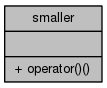
\includegraphics[width=152pt]{structsmaller__coll__graph}
\end{center}
\end{figure}
\subsection*{Public Member Functions}
\begin{DoxyCompactItemize}
\item 
bool \hyperlink{structsmaller_ad76a76ed9b4fa9d8b9ff1a35988d9a48}{operator()} (const std\+::pair$<$ int, double $>$ p1, const std\+::pair$<$ int, double $>$ p2)
\end{DoxyCompactItemize}


\subsection{Member Function Documentation}
\mbox{\Hypertarget{structsmaller_ad76a76ed9b4fa9d8b9ff1a35988d9a48}\label{structsmaller_ad76a76ed9b4fa9d8b9ff1a35988d9a48}} 
\index{smaller@{smaller}!operator()@{operator()}}
\index{operator()@{operator()}!smaller@{smaller}}
\subsubsection{\texorpdfstring{operator()()}{operator()()}}
{\footnotesize\ttfamily bool smaller\+::operator() (\begin{DoxyParamCaption}\item[{const std\+::pair$<$ int, double $>$}]{p1,  }\item[{const std\+::pair$<$ int, double $>$}]{p2 }\end{DoxyParamCaption})\hspace{0.3cm}{\ttfamily [inline]}}



The documentation for this struct was generated from the following file\+:\begin{DoxyCompactItemize}
\item 
src/\hyperlink{IsolationForest_8cpp}{Isolation\+Forest.\+cpp}\end{DoxyCompactItemize}

\hypertarget{structconvForest_1_1topscore}{}\section{conv\+Forest\+:\+:topscore Struct Reference}
\label{structconvForest_1_1topscore}\index{conv\+Forest\+::topscore@{conv\+Forest\+::topscore}}


Collaboration diagram for conv\+Forest\+:\+:topscore\+:\nopagebreak
\begin{figure}[H]
\begin{center}
\leavevmode
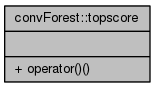
\includegraphics[width=188pt]{structconvForest_1_1topscore__coll__graph}
\end{center}
\end{figure}
\subsection*{Public Member Functions}
\begin{DoxyCompactItemize}
\item 
bool \hyperlink{structconvForest_1_1topscore_aaea88f336c3f2595f2505f6acd0e1958}{operator()} (const std\+::pair$<$ int, double $>$ p1, const std\+::pair$<$ int, double $>$ p2)
\end{DoxyCompactItemize}


\subsection{Member Function Documentation}
\mbox{\Hypertarget{structconvForest_1_1topscore_aaea88f336c3f2595f2505f6acd0e1958}\label{structconvForest_1_1topscore_aaea88f336c3f2595f2505f6acd0e1958}} 
\index{conv\+Forest\+::topscore@{conv\+Forest\+::topscore}!operator()@{operator()}}
\index{operator()@{operator()}!conv\+Forest\+::topscore@{conv\+Forest\+::topscore}}
\subsubsection{\texorpdfstring{operator()()}{operator()()}}
{\footnotesize\ttfamily bool conv\+Forest\+::topscore\+::operator() (\begin{DoxyParamCaption}\item[{const std\+::pair$<$ int, double $>$}]{p1,  }\item[{const std\+::pair$<$ int, double $>$}]{p2 }\end{DoxyParamCaption})\hspace{0.3cm}{\ttfamily [inline]}}



The documentation for this struct was generated from the following file\+:\begin{DoxyCompactItemize}
\item 
src/\hyperlink{convForest_8hpp}{conv\+Forest.\+hpp}\end{DoxyCompactItemize}

\hypertarget{classTree}{}\section{Tree Class Reference}
\label{classTree}\index{Tree@{Tree}}


{\ttfamily \#include $<$Tree.\+hpp$>$}



Inheritance diagram for Tree\+:\nopagebreak
\begin{figure}[H]
\begin{center}
\leavevmode
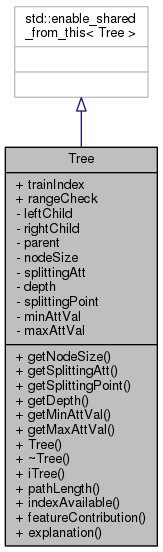
\includegraphics[width=194pt]{classTree__inherit__graph}
\end{center}
\end{figure}


Collaboration diagram for Tree\+:\nopagebreak
\begin{figure}[H]
\begin{center}
\leavevmode
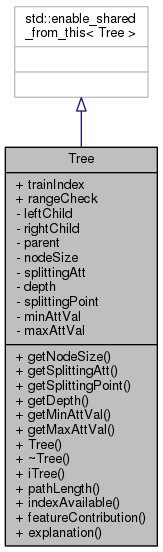
\includegraphics[width=194pt]{classTree__coll__graph}
\end{center}
\end{figure}
\subsection*{Public Member Functions}
\begin{DoxyCompactItemize}
\item 
int \hyperlink{classTree_a0ab54e1652274e304c25473759dcd0da}{get\+Node\+Size} () const
\item 
int \hyperlink{classTree_a877c320f9bed56b1f6d64fc04bd86b97}{get\+Splitting\+Att} () const
\item 
double \hyperlink{classTree_af06e12f440902448730cbe0a7d4fd9a6}{get\+Splitting\+Point} () const
\item 
int \hyperlink{classTree_ad9759be8d8887d04a29ebae7240ced85}{get\+Depth} () const
\item 
double \hyperlink{classTree_a3342558dd44c84ad29c19422f5af4e72}{get\+Min\+Att\+Val} () const
\item 
double \hyperlink{classTree_a70c0b9e6a3a982f6d7c0d38f81019bcf}{get\+Max\+Att\+Val} () const
\item 
\hyperlink{classTree_ad376a7c639d857312f5de2ef47482f68}{Tree} ()
\item 
virtual \hyperlink{classTree_aed209ec340bcf7a378d178e9b41efe44}{$\sim$\+Tree} ()=default
\item 
void \hyperlink{classTree_adf8961073e1d8d7c40c6cb6e6f41bc4c}{i\+Tree} (std\+::vector$<$ int $>$ const \&d\+Index, const doubleframe $\ast$dt, int height, int max\+Height, bool stopheight)
\item 
double \hyperlink{classTree_ad4fdb18020ffddf0250baeeaaaf4e3b5}{path\+Length} (double $\ast$inst)
\item 
bool \hyperlink{classTree_a55ec593d15665c30a9c060db4de09934}{index\+Available} (int index)
\item 
\hyperlink{Contribution_8hpp_a2616a8be768d8598bf3a607996f0f6a4}{contrib} \hyperlink{classTree_a9f3265f93db0eb30a42435d00e26365d}{feature\+Contribution} (double $\ast$inst) const
\item 
std\+::map$<$ int, double $>$ \hyperlink{classTree_a435fa1c641f2abe5e26d36507ba02555}{explanation} (double $\ast$inst)
\end{DoxyCompactItemize}
\subsection*{Data Fields}
\begin{DoxyCompactItemize}
\item 
std\+::vector$<$ int $>$ \hyperlink{classTree_a571ce830364b91f9467f5d464ca119e0}{train\+Index}
\end{DoxyCompactItemize}
\subsection*{Static Public Attributes}
\begin{DoxyCompactItemize}
\item 
static bool \hyperlink{classTree_a0acb952dac4fe2f6321f212402a8f159}{range\+Check}
\end{DoxyCompactItemize}
\subsection*{Private Attributes}
\begin{DoxyCompactItemize}
\item 
std\+::shared\+\_\+ptr$<$ \hyperlink{classTree}{Tree} $>$ \hyperlink{classTree_a6fcca508488527e9028456375504e51e}{left\+Child}
\item 
std\+::shared\+\_\+ptr$<$ \hyperlink{classTree}{Tree} $>$ \hyperlink{classTree_af4d184b80d0e81e70d531911344a418b}{right\+Child}
\item 
std\+::shared\+\_\+ptr$<$ \hyperlink{classTree}{Tree} $>$ \hyperlink{classTree_ae042f82923500e0d34b82510cd02789a}{parent}
\item 
int \hyperlink{classTree_a3748ddc223ca3f6816de3f631026eb73}{node\+Size}
\item 
int \hyperlink{classTree_aae862b9dbe28c1f9d14ad408569b3078}{splitting\+Att}
\item 
int \hyperlink{classTree_aee829f12b9755333a0196190fbe07f1b}{depth}
\item 
double \hyperlink{classTree_a0aeb8a2115f635608ca9a9b0304d304c}{splitting\+Point}
\item 
double \hyperlink{classTree_a8f68db34d3b557765890aeb92f5d6f38}{min\+Att\+Val}
\item 
double \hyperlink{classTree_a4434a97ce3969349d711c0830df1661c}{max\+Att\+Val}
\end{DoxyCompactItemize}


\subsection{Constructor \& Destructor Documentation}
\mbox{\Hypertarget{classTree_ad376a7c639d857312f5de2ef47482f68}\label{classTree_ad376a7c639d857312f5de2ef47482f68}} 
\index{Tree@{Tree}!Tree@{Tree}}
\index{Tree@{Tree}!Tree@{Tree}}
\subsubsection{\texorpdfstring{Tree()}{Tree()}}
{\footnotesize\ttfamily Tree\+::\+Tree (\begin{DoxyParamCaption}{ }\end{DoxyParamCaption})\hspace{0.3cm}{\ttfamily [inline]}}

\mbox{\Hypertarget{classTree_aed209ec340bcf7a378d178e9b41efe44}\label{classTree_aed209ec340bcf7a378d178e9b41efe44}} 
\index{Tree@{Tree}!````~Tree@{$\sim$\+Tree}}
\index{````~Tree@{$\sim$\+Tree}!Tree@{Tree}}
\subsubsection{\texorpdfstring{$\sim$\+Tree()}{~Tree()}}
{\footnotesize\ttfamily virtual Tree\+::$\sim$\+Tree (\begin{DoxyParamCaption}{ }\end{DoxyParamCaption})\hspace{0.3cm}{\ttfamily [virtual]}, {\ttfamily [default]}}



\subsection{Member Function Documentation}
\mbox{\Hypertarget{classTree_a435fa1c641f2abe5e26d36507ba02555}\label{classTree_a435fa1c641f2abe5e26d36507ba02555}} 
\index{Tree@{Tree}!explanation@{explanation}}
\index{explanation@{explanation}!Tree@{Tree}}
\subsubsection{\texorpdfstring{explanation()}{explanation()}}
{\footnotesize\ttfamily std\+::map$<$int,double$>$ Tree\+::explanation (\begin{DoxyParamCaption}\item[{double $\ast$}]{inst }\end{DoxyParamCaption})\hspace{0.3cm}{\ttfamily [inline]}}

\mbox{\Hypertarget{classTree_a9f3265f93db0eb30a42435d00e26365d}\label{classTree_a9f3265f93db0eb30a42435d00e26365d}} 
\index{Tree@{Tree}!feature\+Contribution@{feature\+Contribution}}
\index{feature\+Contribution@{feature\+Contribution}!Tree@{Tree}}
\subsubsection{\texorpdfstring{feature\+Contribution()}{featureContribution()}}
{\footnotesize\ttfamily struct \hyperlink{structContrib}{Contrib} Tree\+::feature\+Contribution (\begin{DoxyParamCaption}\item[{double $\ast$}]{inst }\end{DoxyParamCaption}) const}

\mbox{\Hypertarget{classTree_ad9759be8d8887d04a29ebae7240ced85}\label{classTree_ad9759be8d8887d04a29ebae7240ced85}} 
\index{Tree@{Tree}!get\+Depth@{get\+Depth}}
\index{get\+Depth@{get\+Depth}!Tree@{Tree}}
\subsubsection{\texorpdfstring{get\+Depth()}{getDepth()}}
{\footnotesize\ttfamily int Tree\+::get\+Depth (\begin{DoxyParamCaption}{ }\end{DoxyParamCaption}) const}

\mbox{\Hypertarget{classTree_a70c0b9e6a3a982f6d7c0d38f81019bcf}\label{classTree_a70c0b9e6a3a982f6d7c0d38f81019bcf}} 
\index{Tree@{Tree}!get\+Max\+Att\+Val@{get\+Max\+Att\+Val}}
\index{get\+Max\+Att\+Val@{get\+Max\+Att\+Val}!Tree@{Tree}}
\subsubsection{\texorpdfstring{get\+Max\+Att\+Val()}{getMaxAttVal()}}
{\footnotesize\ttfamily double Tree\+::get\+Max\+Att\+Val (\begin{DoxyParamCaption}{ }\end{DoxyParamCaption}) const}

\mbox{\Hypertarget{classTree_a3342558dd44c84ad29c19422f5af4e72}\label{classTree_a3342558dd44c84ad29c19422f5af4e72}} 
\index{Tree@{Tree}!get\+Min\+Att\+Val@{get\+Min\+Att\+Val}}
\index{get\+Min\+Att\+Val@{get\+Min\+Att\+Val}!Tree@{Tree}}
\subsubsection{\texorpdfstring{get\+Min\+Att\+Val()}{getMinAttVal()}}
{\footnotesize\ttfamily double Tree\+::get\+Min\+Att\+Val (\begin{DoxyParamCaption}{ }\end{DoxyParamCaption}) const}

\mbox{\Hypertarget{classTree_a0ab54e1652274e304c25473759dcd0da}\label{classTree_a0ab54e1652274e304c25473759dcd0da}} 
\index{Tree@{Tree}!get\+Node\+Size@{get\+Node\+Size}}
\index{get\+Node\+Size@{get\+Node\+Size}!Tree@{Tree}}
\subsubsection{\texorpdfstring{get\+Node\+Size()}{getNodeSize()}}
{\footnotesize\ttfamily int Tree\+::get\+Node\+Size (\begin{DoxyParamCaption}{ }\end{DoxyParamCaption}) const}

\mbox{\Hypertarget{classTree_a877c320f9bed56b1f6d64fc04bd86b97}\label{classTree_a877c320f9bed56b1f6d64fc04bd86b97}} 
\index{Tree@{Tree}!get\+Splitting\+Att@{get\+Splitting\+Att}}
\index{get\+Splitting\+Att@{get\+Splitting\+Att}!Tree@{Tree}}
\subsubsection{\texorpdfstring{get\+Splitting\+Att()}{getSplittingAtt()}}
{\footnotesize\ttfamily int Tree\+::get\+Splitting\+Att (\begin{DoxyParamCaption}{ }\end{DoxyParamCaption}) const}

\mbox{\Hypertarget{classTree_af06e12f440902448730cbe0a7d4fd9a6}\label{classTree_af06e12f440902448730cbe0a7d4fd9a6}} 
\index{Tree@{Tree}!get\+Splitting\+Point@{get\+Splitting\+Point}}
\index{get\+Splitting\+Point@{get\+Splitting\+Point}!Tree@{Tree}}
\subsubsection{\texorpdfstring{get\+Splitting\+Point()}{getSplittingPoint()}}
{\footnotesize\ttfamily double Tree\+::get\+Splitting\+Point (\begin{DoxyParamCaption}{ }\end{DoxyParamCaption}) const}

\mbox{\Hypertarget{classTree_a55ec593d15665c30a9c060db4de09934}\label{classTree_a55ec593d15665c30a9c060db4de09934}} 
\index{Tree@{Tree}!index\+Available@{index\+Available}}
\index{index\+Available@{index\+Available}!Tree@{Tree}}
\subsubsection{\texorpdfstring{index\+Available()}{indexAvailable()}}
{\footnotesize\ttfamily bool Tree\+::index\+Available (\begin{DoxyParamCaption}\item[{int}]{index }\end{DoxyParamCaption})}

\mbox{\Hypertarget{classTree_adf8961073e1d8d7c40c6cb6e6f41bc4c}\label{classTree_adf8961073e1d8d7c40c6cb6e6f41bc4c}} 
\index{Tree@{Tree}!i\+Tree@{i\+Tree}}
\index{i\+Tree@{i\+Tree}!Tree@{Tree}}
\subsubsection{\texorpdfstring{i\+Tree()}{iTree()}}
{\footnotesize\ttfamily void Tree\+::i\+Tree (\begin{DoxyParamCaption}\item[{std\+::vector$<$ int $>$ const \&}]{d\+Index,  }\item[{const doubleframe $\ast$}]{dt,  }\item[{int}]{height,  }\item[{int}]{max\+Height,  }\item[{bool}]{stopheight }\end{DoxyParamCaption})}

\mbox{\Hypertarget{classTree_ad4fdb18020ffddf0250baeeaaaf4e3b5}\label{classTree_ad4fdb18020ffddf0250baeeaaaf4e3b5}} 
\index{Tree@{Tree}!path\+Length@{path\+Length}}
\index{path\+Length@{path\+Length}!Tree@{Tree}}
\subsubsection{\texorpdfstring{path\+Length()}{pathLength()}}
{\footnotesize\ttfamily double Tree\+::path\+Length (\begin{DoxyParamCaption}\item[{double $\ast$}]{inst }\end{DoxyParamCaption})}

referenced as null for some input data . 

\subsection{Field Documentation}
\mbox{\Hypertarget{classTree_aee829f12b9755333a0196190fbe07f1b}\label{classTree_aee829f12b9755333a0196190fbe07f1b}} 
\index{Tree@{Tree}!depth@{depth}}
\index{depth@{depth}!Tree@{Tree}}
\subsubsection{\texorpdfstring{depth}{depth}}
{\footnotesize\ttfamily int Tree\+::depth\hspace{0.3cm}{\ttfamily [private]}}

\mbox{\Hypertarget{classTree_a6fcca508488527e9028456375504e51e}\label{classTree_a6fcca508488527e9028456375504e51e}} 
\index{Tree@{Tree}!left\+Child@{left\+Child}}
\index{left\+Child@{left\+Child}!Tree@{Tree}}
\subsubsection{\texorpdfstring{left\+Child}{leftChild}}
{\footnotesize\ttfamily std\+::shared\+\_\+ptr$<$\hyperlink{classTree}{Tree}$>$ Tree\+::left\+Child\hspace{0.3cm}{\ttfamily [private]}}

\mbox{\Hypertarget{classTree_a4434a97ce3969349d711c0830df1661c}\label{classTree_a4434a97ce3969349d711c0830df1661c}} 
\index{Tree@{Tree}!max\+Att\+Val@{max\+Att\+Val}}
\index{max\+Att\+Val@{max\+Att\+Val}!Tree@{Tree}}
\subsubsection{\texorpdfstring{max\+Att\+Val}{maxAttVal}}
{\footnotesize\ttfamily double Tree\+::max\+Att\+Val\hspace{0.3cm}{\ttfamily [private]}}

\mbox{\Hypertarget{classTree_a8f68db34d3b557765890aeb92f5d6f38}\label{classTree_a8f68db34d3b557765890aeb92f5d6f38}} 
\index{Tree@{Tree}!min\+Att\+Val@{min\+Att\+Val}}
\index{min\+Att\+Val@{min\+Att\+Val}!Tree@{Tree}}
\subsubsection{\texorpdfstring{min\+Att\+Val}{minAttVal}}
{\footnotesize\ttfamily double Tree\+::min\+Att\+Val\hspace{0.3cm}{\ttfamily [private]}}

\mbox{\Hypertarget{classTree_a3748ddc223ca3f6816de3f631026eb73}\label{classTree_a3748ddc223ca3f6816de3f631026eb73}} 
\index{Tree@{Tree}!node\+Size@{node\+Size}}
\index{node\+Size@{node\+Size}!Tree@{Tree}}
\subsubsection{\texorpdfstring{node\+Size}{nodeSize}}
{\footnotesize\ttfamily int Tree\+::node\+Size\hspace{0.3cm}{\ttfamily [private]}}

\mbox{\Hypertarget{classTree_ae042f82923500e0d34b82510cd02789a}\label{classTree_ae042f82923500e0d34b82510cd02789a}} 
\index{Tree@{Tree}!parent@{parent}}
\index{parent@{parent}!Tree@{Tree}}
\subsubsection{\texorpdfstring{parent}{parent}}
{\footnotesize\ttfamily std\+::shared\+\_\+ptr$<$\hyperlink{classTree}{Tree}$>$ Tree\+::parent\hspace{0.3cm}{\ttfamily [private]}}

\mbox{\Hypertarget{classTree_a0acb952dac4fe2f6321f212402a8f159}\label{classTree_a0acb952dac4fe2f6321f212402a8f159}} 
\index{Tree@{Tree}!range\+Check@{range\+Check}}
\index{range\+Check@{range\+Check}!Tree@{Tree}}
\subsubsection{\texorpdfstring{range\+Check}{rangeCheck}}
{\footnotesize\ttfamily bool Tree\+::range\+Check\hspace{0.3cm}{\ttfamily [static]}}

\mbox{\Hypertarget{classTree_af4d184b80d0e81e70d531911344a418b}\label{classTree_af4d184b80d0e81e70d531911344a418b}} 
\index{Tree@{Tree}!right\+Child@{right\+Child}}
\index{right\+Child@{right\+Child}!Tree@{Tree}}
\subsubsection{\texorpdfstring{right\+Child}{rightChild}}
{\footnotesize\ttfamily std\+::shared\+\_\+ptr$<$\hyperlink{classTree}{Tree}$>$ Tree\+::right\+Child\hspace{0.3cm}{\ttfamily [private]}}

\mbox{\Hypertarget{classTree_aae862b9dbe28c1f9d14ad408569b3078}\label{classTree_aae862b9dbe28c1f9d14ad408569b3078}} 
\index{Tree@{Tree}!splitting\+Att@{splitting\+Att}}
\index{splitting\+Att@{splitting\+Att}!Tree@{Tree}}
\subsubsection{\texorpdfstring{splitting\+Att}{splittingAtt}}
{\footnotesize\ttfamily int Tree\+::splitting\+Att\hspace{0.3cm}{\ttfamily [private]}}

\mbox{\Hypertarget{classTree_a0aeb8a2115f635608ca9a9b0304d304c}\label{classTree_a0aeb8a2115f635608ca9a9b0304d304c}} 
\index{Tree@{Tree}!splitting\+Point@{splitting\+Point}}
\index{splitting\+Point@{splitting\+Point}!Tree@{Tree}}
\subsubsection{\texorpdfstring{splitting\+Point}{splittingPoint}}
{\footnotesize\ttfamily double Tree\+::splitting\+Point\hspace{0.3cm}{\ttfamily [private]}}

\mbox{\Hypertarget{classTree_a571ce830364b91f9467f5d464ca119e0}\label{classTree_a571ce830364b91f9467f5d464ca119e0}} 
\index{Tree@{Tree}!train\+Index@{train\+Index}}
\index{train\+Index@{train\+Index}!Tree@{Tree}}
\subsubsection{\texorpdfstring{train\+Index}{trainIndex}}
{\footnotesize\ttfamily std\+::vector$<$int$>$ Tree\+::train\+Index}



The documentation for this class was generated from the following files\+:\begin{DoxyCompactItemize}
\item 
src/\hyperlink{Tree_8hpp}{Tree.\+hpp}\item 
src/\hyperlink{Tree_8cpp}{Tree.\+cpp}\end{DoxyCompactItemize}

\chapter{File Documentation}
\hypertarget{BootstrapConvergence_8cpp}{}\section{src/\+Bootstrap\+Convergence.cpp File Reference}
\label{BootstrapConvergence_8cpp}\index{src/\+Bootstrap\+Convergence.\+cpp@{src/\+Bootstrap\+Convergence.\+cpp}}
{\ttfamily \#include \char`\"{}Bootstrap\+Convergence.\+hpp\char`\"{}}\newline
Include dependency graph for Bootstrap\+Convergence.\+cpp\+:\nopagebreak
\begin{figure}[H]
\begin{center}
\leavevmode
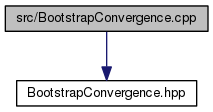
\includegraphics[width=232pt]{BootstrapConvergence_8cpp__incl}
\end{center}
\end{figure}

\hypertarget{BootstrapConvergence_8hpp}{}\section{src/\+Bootstrap\+Convergence.hpp File Reference}
\label{BootstrapConvergence_8hpp}\index{src/\+Bootstrap\+Convergence.\+hpp@{src/\+Bootstrap\+Convergence.\+hpp}}
This graph shows which files directly or indirectly include this file\+:\nopagebreak
\begin{figure}[H]
\begin{center}
\leavevmode
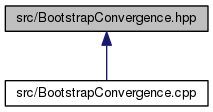
\includegraphics[width=232pt]{BootstrapConvergence_8hpp__dep__incl}
\end{center}
\end{figure}
\subsection*{Data Structures}
\begin{DoxyCompactItemize}
\item 
class \hyperlink{classBootstrapConvergence}{Bootstrap\+Convergence}
\end{DoxyCompactItemize}

\hypertarget{cincl_8hpp}{}\section{src/cincl.hpp File Reference}
\label{cincl_8hpp}\index{src/cincl.\+hpp@{src/cincl.\+hpp}}
{\ttfamily \#include \char`\"{}C/common.\+h\char`\"{}}\newline
{\ttfamily \#include \char`\"{}C/object.\+h\char`\"{}}\newline
{\ttfamily \#include \char`\"{}C/strfun.\+h\char`\"{}}\newline
{\ttfamily \#include \char`\"{}C/readwrite.\+h\char`\"{}}\newline
{\ttfamily \#include \char`\"{}C/frames.\+h\char`\"{}}\newline
{\ttfamily \#include \char`\"{}C/argparse.\+h\char`\"{}}\newline
{\ttfamily \#include \char`\"{}C/argparse\+\_\+iforest.\+h\char`\"{}}\newline
Include dependency graph for cincl.\+hpp\+:\nopagebreak
\begin{figure}[H]
\begin{center}
\leavevmode
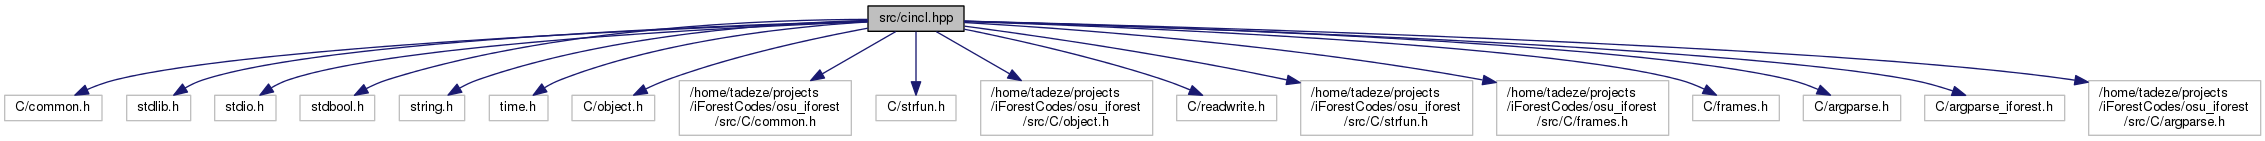
\includegraphics[width=350pt]{cincl_8hpp__incl}
\end{center}
\end{figure}
This graph shows which files directly or indirectly include this file\+:\nopagebreak
\begin{figure}[H]
\begin{center}
\leavevmode
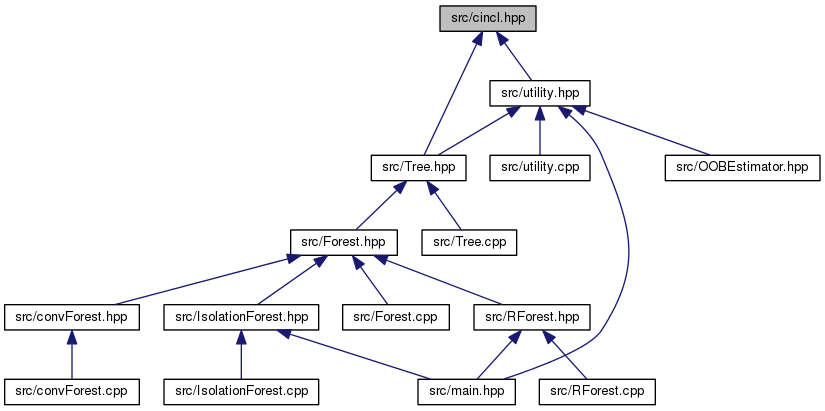
\includegraphics[width=350pt]{cincl_8hpp__dep__incl}
\end{center}
\end{figure}

\hypertarget{Contribution_8hpp}{}\section{src/\+Contribution.hpp File Reference}
\label{Contribution_8hpp}\index{src/\+Contribution.\+hpp@{src/\+Contribution.\+hpp}}
{\ttfamily \#include $<$vector$>$}\newline
{\ttfamily \#include $<$map$>$}\newline
Include dependency graph for Contribution.\+hpp\+:\nopagebreak
\begin{figure}[H]
\begin{center}
\leavevmode
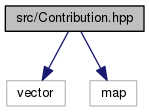
\includegraphics[width=184pt]{Contribution_8hpp__incl}
\end{center}
\end{figure}
This graph shows which files directly or indirectly include this file\+:\nopagebreak
\begin{figure}[H]
\begin{center}
\leavevmode
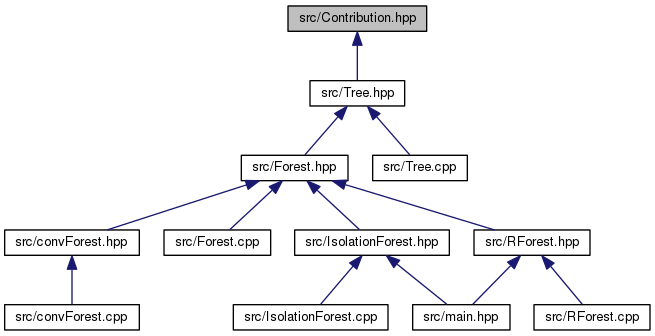
\includegraphics[width=350pt]{Contribution_8hpp__dep__incl}
\end{center}
\end{figure}
\subsection*{Data Structures}
\begin{DoxyCompactItemize}
\item 
struct \hyperlink{structContrib}{Contrib}
\end{DoxyCompactItemize}
\subsection*{Typedefs}
\begin{DoxyCompactItemize}
\item 
using \hyperlink{Contribution_8hpp_a2616a8be768d8598bf3a607996f0f6a4}{contrib} = struct \hyperlink{structContrib}{Contrib}
\end{DoxyCompactItemize}


\subsection{Typedef Documentation}
\mbox{\Hypertarget{Contribution_8hpp_a2616a8be768d8598bf3a607996f0f6a4}\label{Contribution_8hpp_a2616a8be768d8598bf3a607996f0f6a4}} 
\index{Contribution.\+hpp@{Contribution.\+hpp}!contrib@{contrib}}
\index{contrib@{contrib}!Contribution.\+hpp@{Contribution.\+hpp}}
\subsubsection{\texorpdfstring{contrib}{contrib}}
{\footnotesize\ttfamily using \hyperlink{Contribution_8hpp_a2616a8be768d8598bf3a607996f0f6a4}{contrib} =  struct \hyperlink{structContrib}{Contrib}}


\hypertarget{convForest_8cpp}{}\section{src/conv\+Forest.cpp File Reference}
\label{convForest_8cpp}\index{src/conv\+Forest.\+cpp@{src/conv\+Forest.\+cpp}}
{\ttfamily \#include \char`\"{}conv\+Forest.\+hpp\char`\"{}}\newline
Include dependency graph for conv\+Forest.\+cpp\+:\nopagebreak
\begin{figure}[H]
\begin{center}
\leavevmode
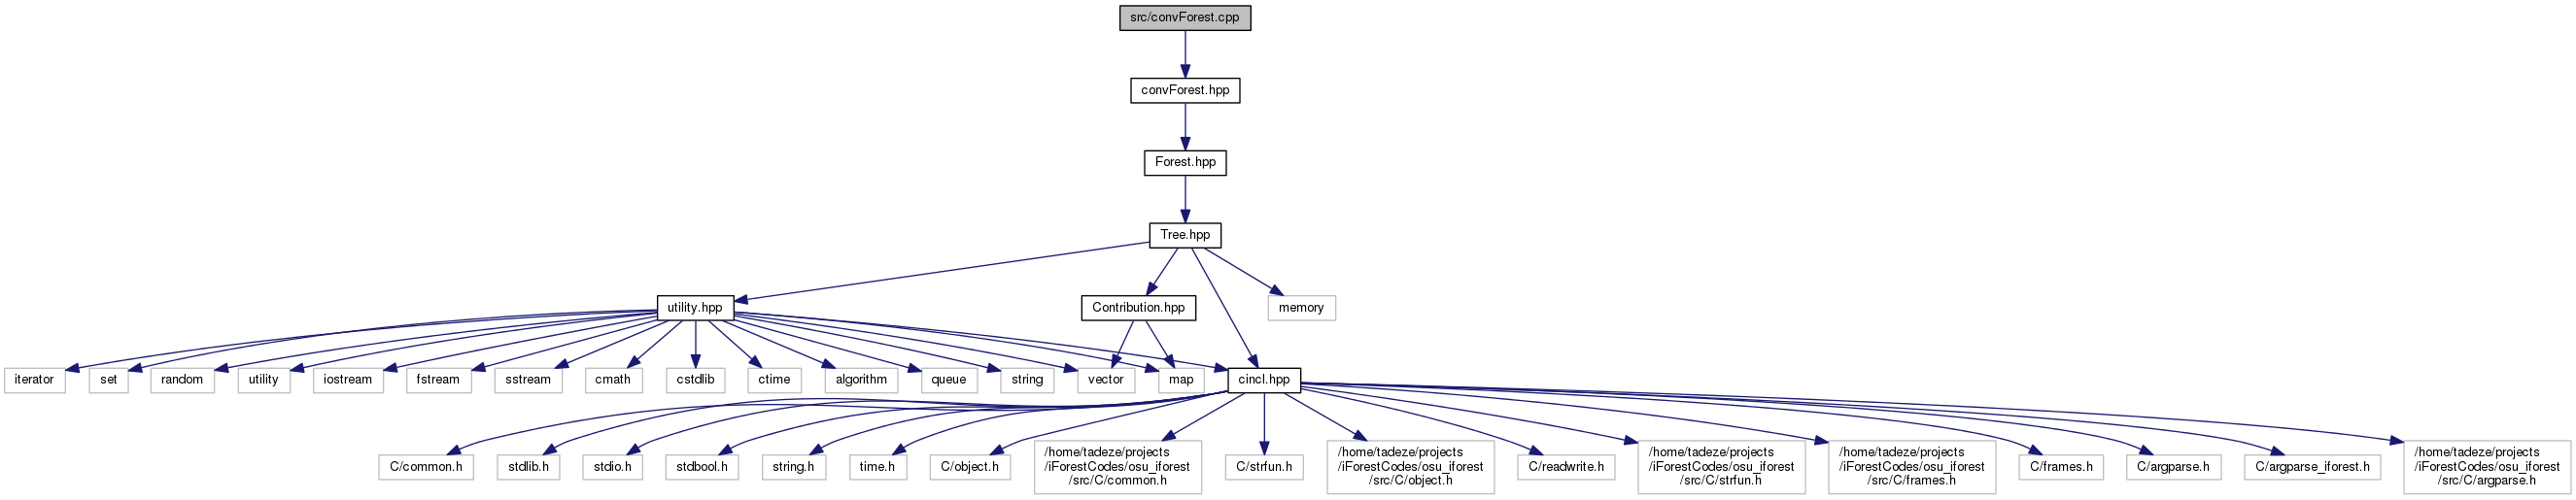
\includegraphics[width=350pt]{convForest_8cpp__incl}
\end{center}
\end{figure}

\hypertarget{convForest_8hpp}{}\section{src/conv\+Forest.hpp File Reference}
\label{convForest_8hpp}\index{src/conv\+Forest.\+hpp@{src/conv\+Forest.\+hpp}}
{\ttfamily \#include \char`\"{}Forest.\+hpp\char`\"{}}\newline
Include dependency graph for conv\+Forest.\+hpp\+:\nopagebreak
\begin{figure}[H]
\begin{center}
\leavevmode
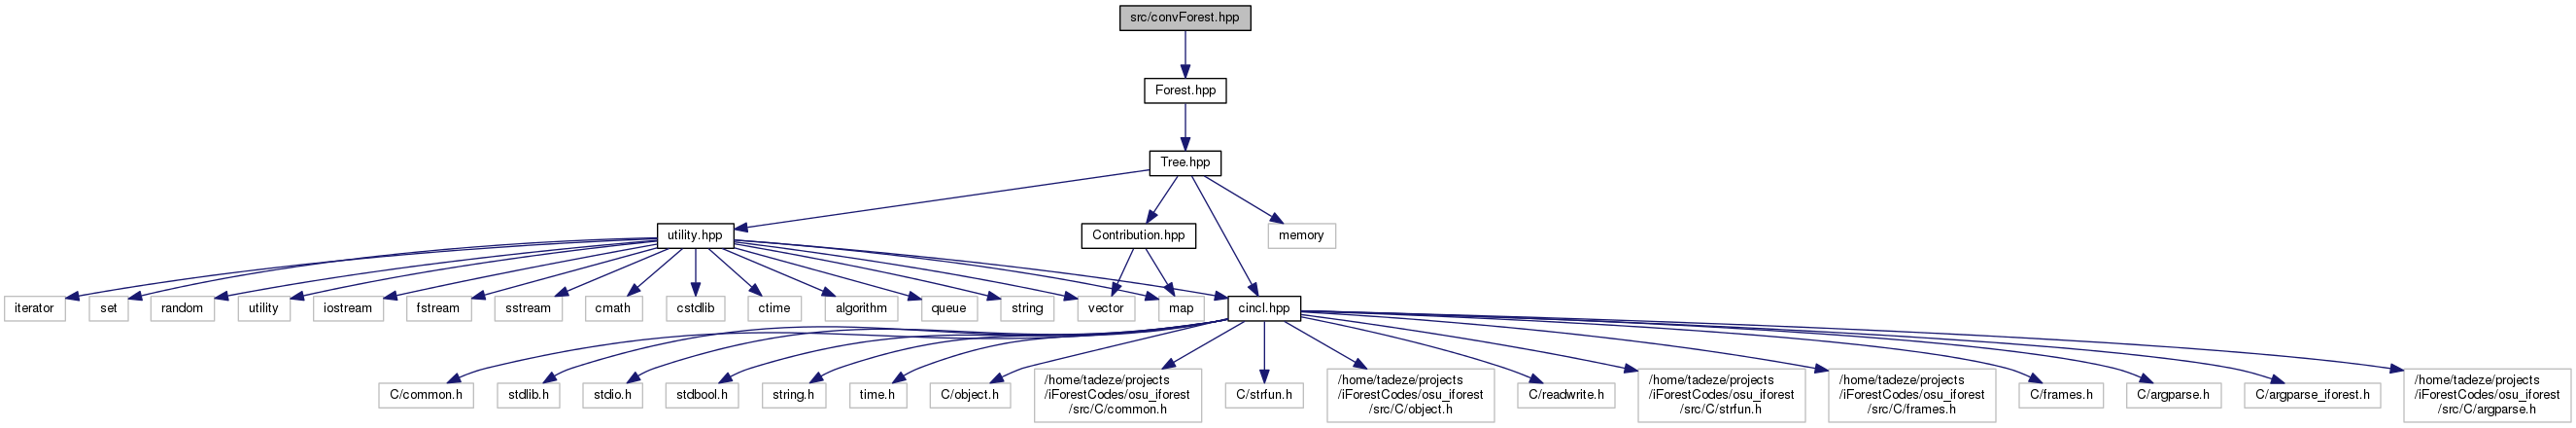
\includegraphics[width=350pt]{convForest_8hpp__incl}
\end{center}
\end{figure}
This graph shows which files directly or indirectly include this file\+:\nopagebreak
\begin{figure}[H]
\begin{center}
\leavevmode
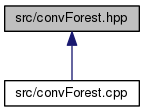
\includegraphics[width=180pt]{convForest_8hpp__dep__incl}
\end{center}
\end{figure}
\subsection*{Data Structures}
\begin{DoxyCompactItemize}
\item 
class \hyperlink{classconvForest}{conv\+Forest}
\item 
struct \hyperlink{structconvForest_1_1topscore}{conv\+Forest\+::topscore}
\item 
struct \hyperlink{structconvForest_1_1larger}{conv\+Forest\+::larger}
\end{DoxyCompactItemize}

\hypertarget{Forest_8cpp}{}\section{src/\+Forest.cpp File Reference}
\label{Forest_8cpp}\index{src/\+Forest.\+cpp@{src/\+Forest.\+cpp}}
{\ttfamily \#include \char`\"{}Forest.\+hpp\char`\"{}}\newline
Include dependency graph for Forest.\+cpp\+:\nopagebreak
\begin{figure}[H]
\begin{center}
\leavevmode
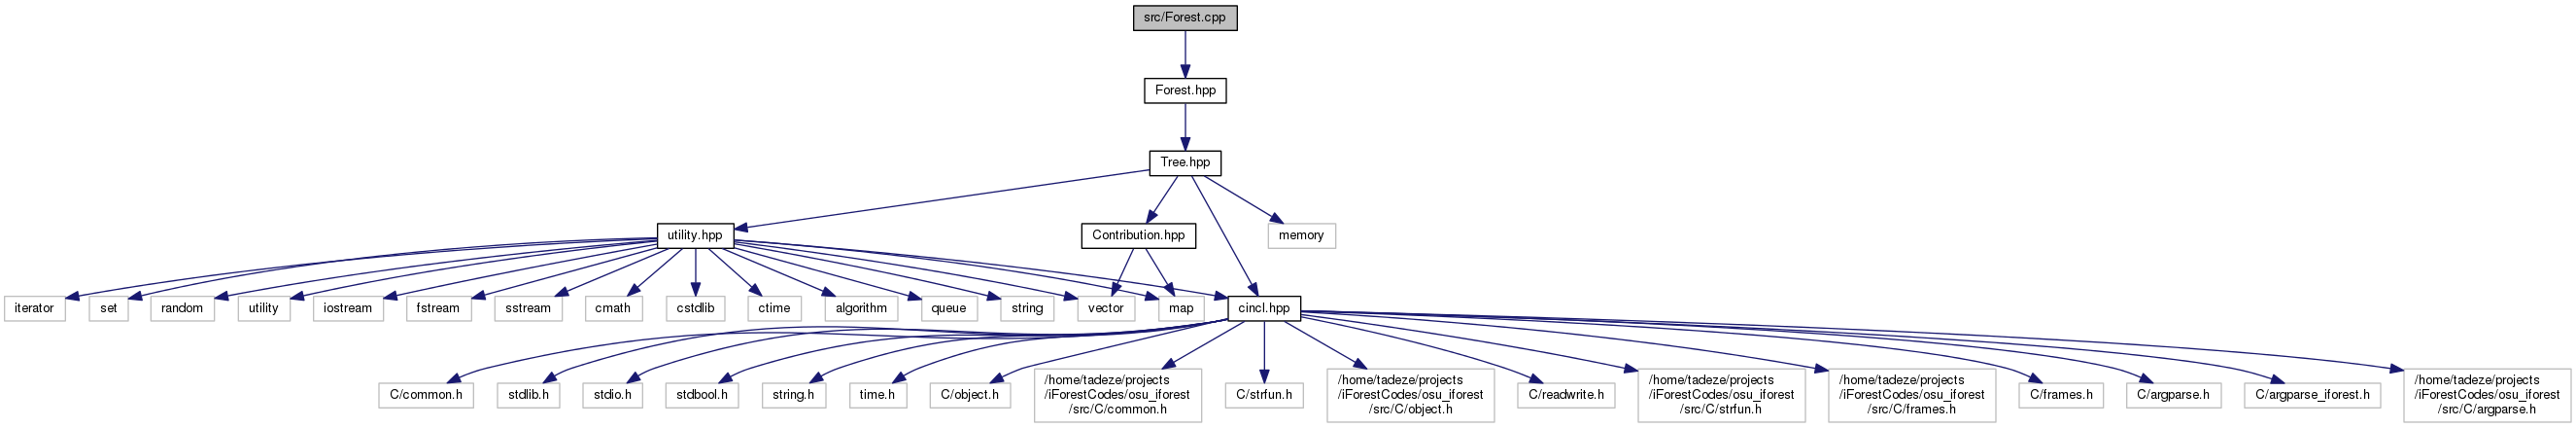
\includegraphics[width=350pt]{Forest_8cpp__incl}
\end{center}
\end{figure}
\subsection*{Functions}
\begin{DoxyCompactItemize}
\item 
{\footnotesize template$<$class T $>$ }\\double \hyperlink{Forest_8cpp_afcb1091a2ec66c0e1e3788a595b92b4c}{oob\+Mean\+Depth} (std\+::vector$<$ T $>$ \&vec)
\end{DoxyCompactItemize}


\subsection{Function Documentation}
\mbox{\Hypertarget{Forest_8cpp_afcb1091a2ec66c0e1e3788a595b92b4c}\label{Forest_8cpp_afcb1091a2ec66c0e1e3788a595b92b4c}} 
\index{Forest.\+cpp@{Forest.\+cpp}!oob\+Mean\+Depth@{oob\+Mean\+Depth}}
\index{oob\+Mean\+Depth@{oob\+Mean\+Depth}!Forest.\+cpp@{Forest.\+cpp}}
\subsubsection{\texorpdfstring{oob\+Mean\+Depth()}{oobMeanDepth()}}
{\footnotesize\ttfamily template$<$class T $>$ \\
double oob\+Mean\+Depth (\begin{DoxyParamCaption}\item[{std\+::vector$<$ T $>$ \&}]{vec }\end{DoxyParamCaption})}


\hypertarget{Forest_8hpp}{}\section{src/\+Forest.hpp File Reference}
\label{Forest_8hpp}\index{src/\+Forest.\+hpp@{src/\+Forest.\+hpp}}
{\ttfamily \#include \char`\"{}Tree.\+hpp\char`\"{}}\newline
Include dependency graph for Forest.\+hpp\+:\nopagebreak
\begin{figure}[H]
\begin{center}
\leavevmode
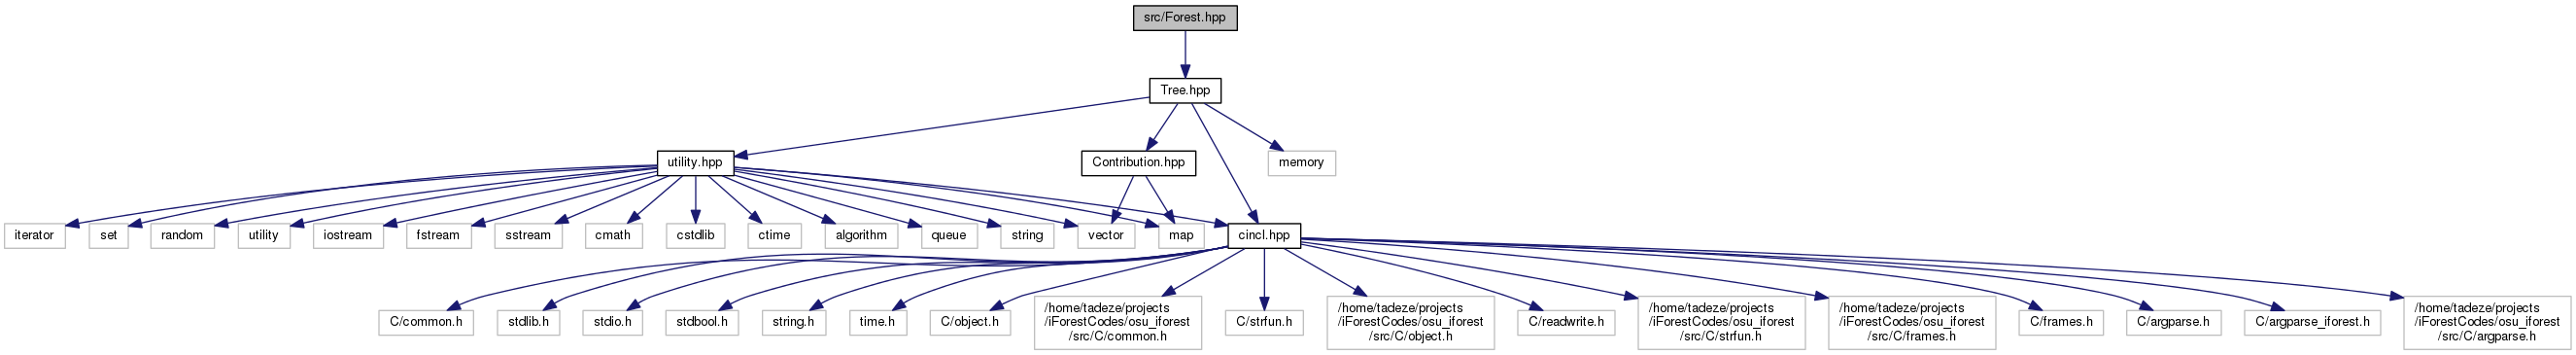
\includegraphics[width=350pt]{Forest_8hpp__incl}
\end{center}
\end{figure}
This graph shows which files directly or indirectly include this file\+:\nopagebreak
\begin{figure}[H]
\begin{center}
\leavevmode
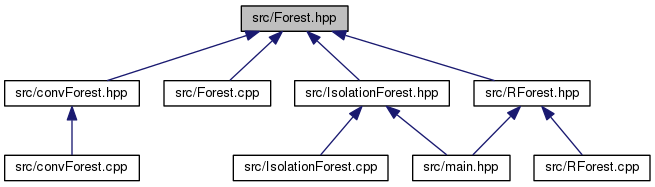
\includegraphics[width=350pt]{Forest_8hpp__dep__incl}
\end{center}
\end{figure}
\subsection*{Data Structures}
\begin{DoxyCompactItemize}
\item 
class \hyperlink{classForest}{Forest}
\item 
struct \hyperlink{structForest_1_1larger}{Forest\+::larger}
\end{DoxyCompactItemize}

\hypertarget{IsolationForest_8cpp}{}\section{src/\+Isolation\+Forest.cpp File Reference}
\label{IsolationForest_8cpp}\index{src/\+Isolation\+Forest.\+cpp@{src/\+Isolation\+Forest.\+cpp}}
{\ttfamily \#include \char`\"{}Isolation\+Forest.\+hpp\char`\"{}}\newline
Include dependency graph for Isolation\+Forest.\+cpp\+:\nopagebreak
\begin{figure}[H]
\begin{center}
\leavevmode
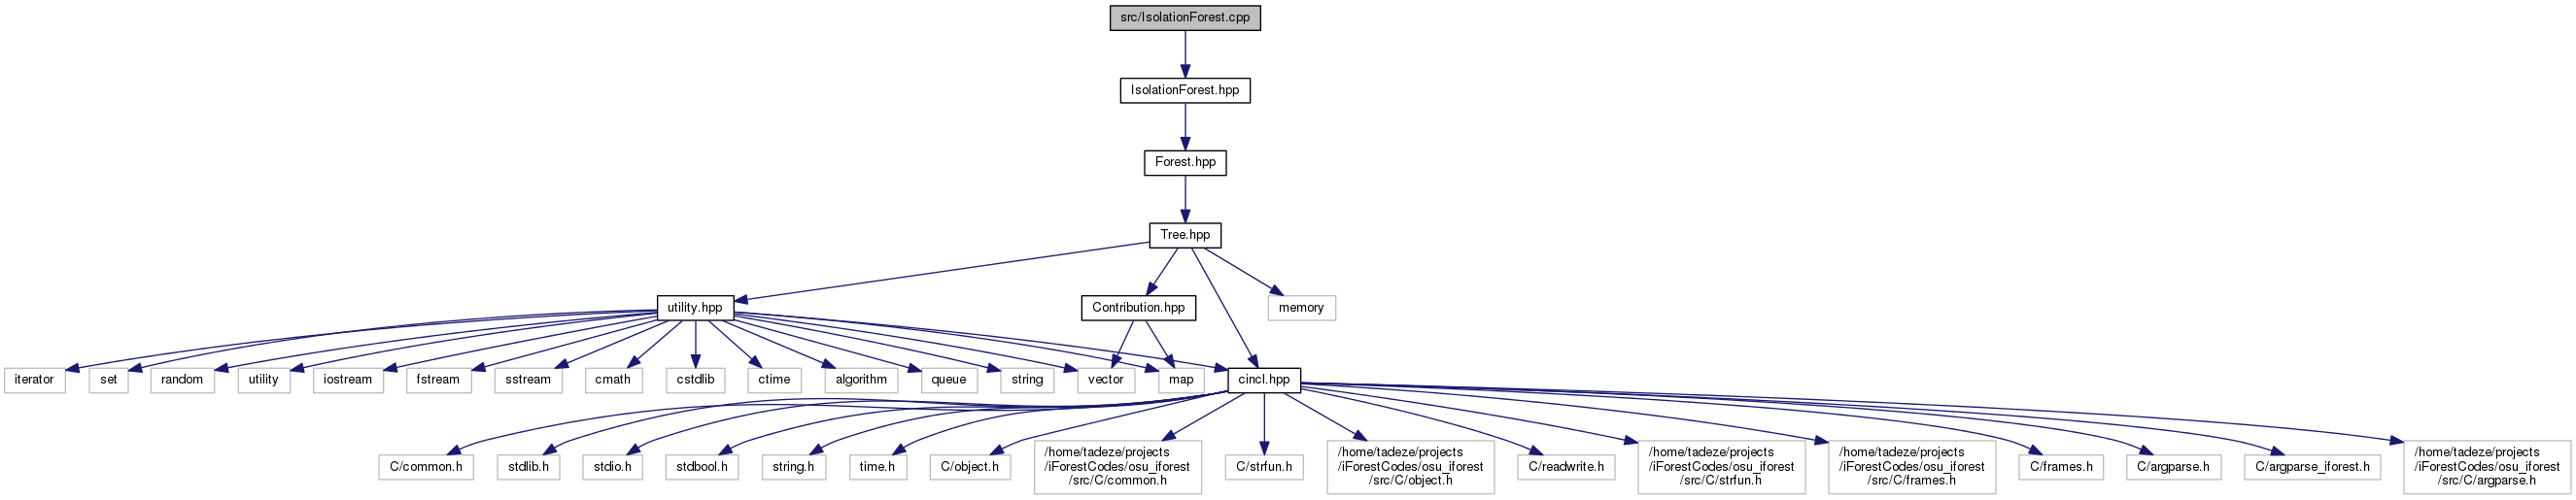
\includegraphics[width=350pt]{IsolationForest_8cpp__incl}
\end{center}
\end{figure}
\subsection*{Data Structures}
\begin{DoxyCompactItemize}
\item 
struct \hyperlink{structsmaller}{smaller}
\end{DoxyCompactItemize}

\hypertarget{IsolationForest_8hpp}{}\section{src/\+Isolation\+Forest.hpp File Reference}
\label{IsolationForest_8hpp}\index{src/\+Isolation\+Forest.\+hpp@{src/\+Isolation\+Forest.\+hpp}}
{\ttfamily \#include \char`\"{}Forest.\+hpp\char`\"{}}\newline
Include dependency graph for Isolation\+Forest.\+hpp\+:\nopagebreak
\begin{figure}[H]
\begin{center}
\leavevmode
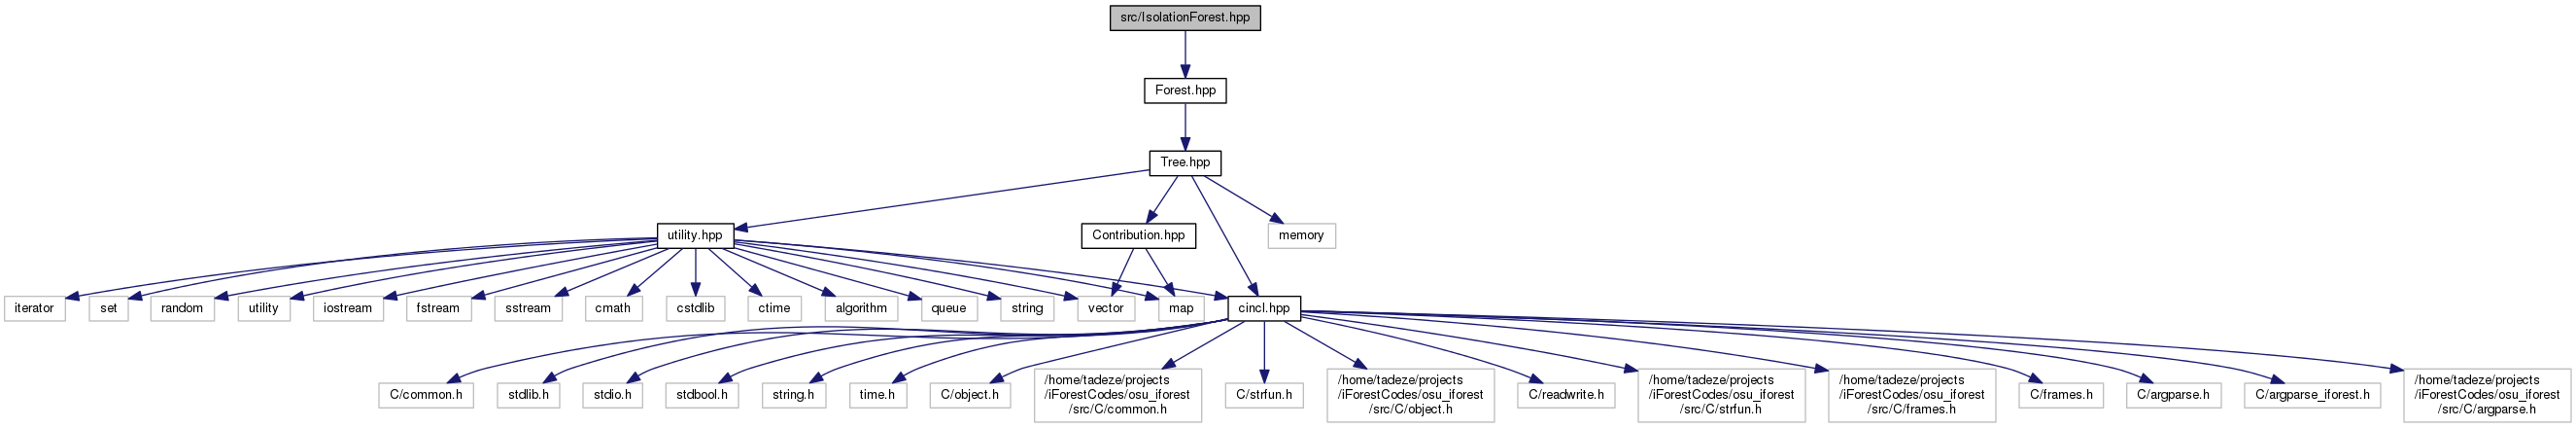
\includegraphics[width=350pt]{IsolationForest_8hpp__incl}
\end{center}
\end{figure}
This graph shows which files directly or indirectly include this file\+:\nopagebreak
\begin{figure}[H]
\begin{center}
\leavevmode
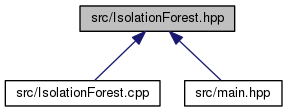
\includegraphics[width=287pt]{IsolationForest_8hpp__dep__incl}
\end{center}
\end{figure}
\subsection*{Data Structures}
\begin{DoxyCompactItemize}
\item 
class \hyperlink{classIsolationForest}{Isolation\+Forest}
\end{DoxyCompactItemize}

\hypertarget{main_8hpp}{}\section{src/main.hpp File Reference}
\label{main_8hpp}\index{src/main.\+hpp@{src/main.\+hpp}}
{\ttfamily \#include \char`\"{}R\+Forest.\+hpp\char`\"{}}\newline
{\ttfamily \#include \char`\"{}Isolation\+Forest.\+hpp\char`\"{}}\newline
{\ttfamily \#include \char`\"{}utility.\+hpp\char`\"{}}\newline
\subsection*{Functions}
\begin{DoxyCompactItemize}
\item 
void \hyperlink{main_8hpp_a3aeb3231e1f45927033953edceb8ba8f}{build\+Forest} (std\+::shared\+\_\+ptr$<$ \hyperlink{classForest}{Forest} $>$ iff, doubleframe $\ast$test\+\_\+dt, const double alpha, int stop\+Limit, float rho, std\+::string output\+\_\+name, ntstringframe $\ast$metadata, bool save\+Path\+Length)
\item 
void \hyperlink{main_8hpp_a1c88fd9a519ace3815ae39af2258b9eb}{save\+Score\+To\+File} (std\+::vector$<$ double $>$ \&scores, std\+::vector$<$ std\+::vector$<$ double $>$ $>$ \&path\+Length, const ntstringframe $\ast$metadata, std\+::string f\+Name, bool save\+Path\+Length)
\end{DoxyCompactItemize}


\subsection{Function Documentation}
\mbox{\Hypertarget{main_8hpp_a3aeb3231e1f45927033953edceb8ba8f}\label{main_8hpp_a3aeb3231e1f45927033953edceb8ba8f}} 
\index{main.\+hpp@{main.\+hpp}!build\+Forest@{build\+Forest}}
\index{build\+Forest@{build\+Forest}!main.\+hpp@{main.\+hpp}}
\subsubsection{\texorpdfstring{build\+Forest()}{buildForest()}}
{\footnotesize\ttfamily void build\+Forest (\begin{DoxyParamCaption}\item[{std\+::shared\+\_\+ptr$<$ \hyperlink{classForest}{Forest} $>$}]{iff,  }\item[{doubleframe $\ast$}]{test\+\_\+dt,  }\item[{const double}]{alpha,  }\item[{int}]{stop\+Limit,  }\item[{float}]{rho,  }\item[{std\+::string}]{output\+\_\+name,  }\item[{ntstringframe $\ast$}]{metadata,  }\item[{bool}]{save\+Path\+Length }\end{DoxyParamCaption})}

\mbox{\Hypertarget{main_8hpp_a1c88fd9a519ace3815ae39af2258b9eb}\label{main_8hpp_a1c88fd9a519ace3815ae39af2258b9eb}} 
\index{main.\+hpp@{main.\+hpp}!save\+Score\+To\+File@{save\+Score\+To\+File}}
\index{save\+Score\+To\+File@{save\+Score\+To\+File}!main.\+hpp@{main.\+hpp}}
\subsubsection{\texorpdfstring{save\+Score\+To\+File()}{saveScoreToFile()}}
{\footnotesize\ttfamily void save\+Score\+To\+File (\begin{DoxyParamCaption}\item[{std\+::vector$<$ double $>$ \&}]{scores,  }\item[{std\+::vector$<$ std\+::vector$<$ double $>$ $>$ \&}]{path\+Length,  }\item[{const ntstringframe $\ast$}]{metadata,  }\item[{std\+::string}]{f\+Name,  }\item[{bool}]{save\+Path\+Length }\end{DoxyParamCaption})}


\hypertarget{metric_8cpp}{}\section{src/metric.cpp File Reference}
\label{metric_8cpp}\index{src/metric.\+cpp@{src/metric.\+cpp}}
{\ttfamily \#include \char`\"{}metric.\+hpp\char`\"{}}\newline
Include dependency graph for metric.\+cpp\+:\nopagebreak
\begin{figure}[H]
\begin{center}
\leavevmode
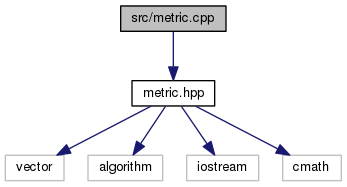
\includegraphics[width=332pt]{metric_8cpp__incl}
\end{center}
\end{figure}
\subsection*{Namespaces}
\begin{DoxyCompactItemize}
\item 
 \hyperlink{namespacemetric}{metric}
\end{DoxyCompactItemize}
\subsection*{Functions}
\begin{DoxyCompactItemize}
\item 
double \hyperlink{namespacemetric_a87e5308fcebc95b5720c24dc70d74349}{metric\+::trapezoid\+Area} (double X1, double X2, double Y1, double Y2)
\item 
double \hyperlink{namespacemetric_a57492bb556d712873ca231e6427a139e}{metric\+::\+A\+UC} (vector$<$ double $>$ \&labels, vector$<$ double $>$ \&scores, int n, int posclass)
\end{DoxyCompactItemize}

\hypertarget{metric_8hpp}{}\section{src/metric.hpp File Reference}
\label{metric_8hpp}\index{src/metric.\+hpp@{src/metric.\+hpp}}
{\ttfamily \#include $<$vector$>$}\newline
{\ttfamily \#include $<$algorithm$>$}\newline
{\ttfamily \#include $<$iostream$>$}\newline
{\ttfamily \#include $<$cmath$>$}\newline
Include dependency graph for metric.\+hpp\+:\nopagebreak
\begin{figure}[H]
\begin{center}
\leavevmode
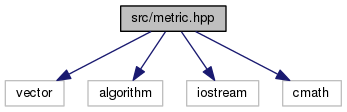
\includegraphics[width=332pt]{metric_8hpp__incl}
\end{center}
\end{figure}
This graph shows which files directly or indirectly include this file\+:\nopagebreak
\begin{figure}[H]
\begin{center}
\leavevmode
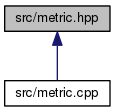
\includegraphics[width=158pt]{metric_8hpp__dep__incl}
\end{center}
\end{figure}
\subsection*{Namespaces}
\begin{DoxyCompactItemize}
\item 
 \hyperlink{namespacemetric}{metric}
\end{DoxyCompactItemize}
\subsection*{Functions}
\begin{DoxyCompactItemize}
\item 
double \hyperlink{namespacemetric_af2bf0a8c7be4bee4eff0abaa603e842e}{metric\+::\+A\+UC} (std\+::vector$<$ double $>$ \&labels, std\+::vector$<$ double $>$ \&scores, int n, int posclass)
\item 
double \hyperlink{namespacemetric_a3db123a20e7cf257d2c3777be1573094}{metric\+::ap} (std\+::vector$<$ double $>$ \&labels, std\+::vector$<$ double $>$ \&scores, int n, int posclass)
\end{DoxyCompactItemize}

\hypertarget{OOBEstimator_8hpp}{}\section{src/\+O\+O\+B\+Estimator.hpp File Reference}
\label{OOBEstimator_8hpp}\index{src/\+O\+O\+B\+Estimator.\+hpp@{src/\+O\+O\+B\+Estimator.\+hpp}}
{\ttfamily \#include \char`\"{}utility.\+hpp\char`\"{}}\newline
Include dependency graph for O\+O\+B\+Estimator.\+hpp\+:\nopagebreak
\begin{figure}[H]
\begin{center}
\leavevmode
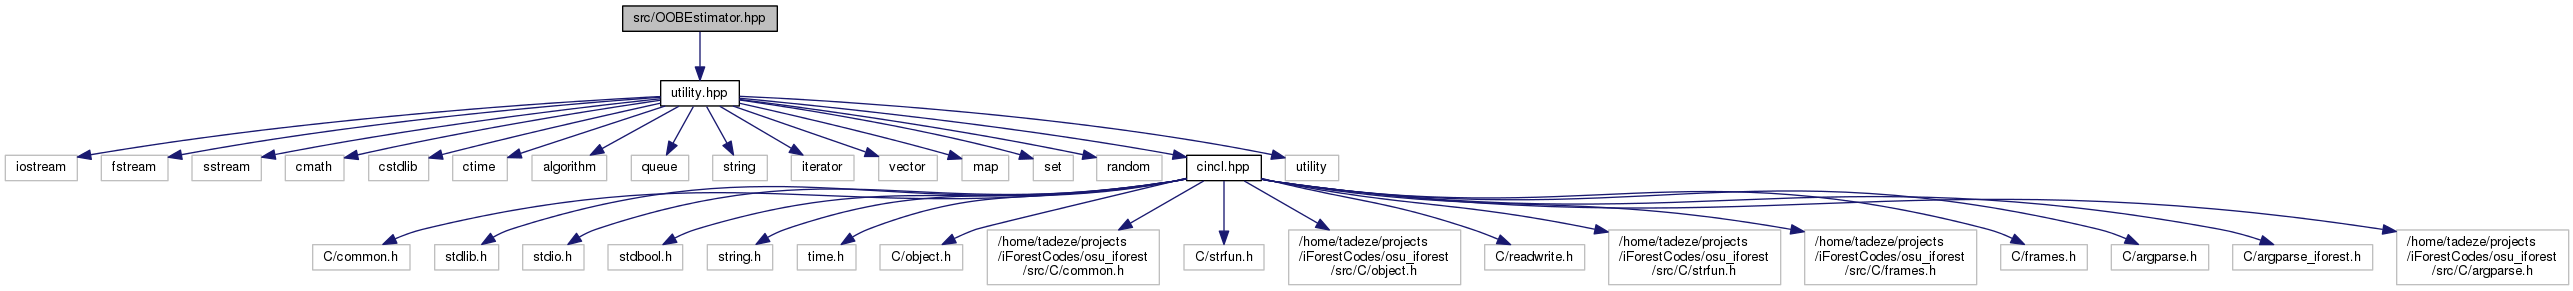
\includegraphics[width=350pt]{OOBEstimator_8hpp__incl}
\end{center}
\end{figure}
\subsection*{Data Structures}
\begin{DoxyCompactItemize}
\item 
struct \hyperlink{structOOBEstimator}{O\+O\+B\+Estimator}
\end{DoxyCompactItemize}
\subsection*{Typedefs}
\begin{DoxyCompactItemize}
\item 
typedef struct \hyperlink{structOOBEstimator}{O\+O\+B\+Estimator} \hyperlink{OOBEstimator_8hpp_a7b1915bb4636724102e0478ff093eff8}{O\+O\+B\+Estimator}
\end{DoxyCompactItemize}


\subsection{Typedef Documentation}
\mbox{\Hypertarget{OOBEstimator_8hpp_a7b1915bb4636724102e0478ff093eff8}\label{OOBEstimator_8hpp_a7b1915bb4636724102e0478ff093eff8}} 
\index{O\+O\+B\+Estimator.\+hpp@{O\+O\+B\+Estimator.\+hpp}!O\+O\+B\+Estimator@{O\+O\+B\+Estimator}}
\index{O\+O\+B\+Estimator@{O\+O\+B\+Estimator}!O\+O\+B\+Estimator.\+hpp@{O\+O\+B\+Estimator.\+hpp}}
\subsubsection{\texorpdfstring{O\+O\+B\+Estimator}{OOBEstimator}}
{\footnotesize\ttfamily typedef struct \hyperlink{structOOBEstimator}{O\+O\+B\+Estimator} \hyperlink{structOOBEstimator}{O\+O\+B\+Estimator}}


\hypertarget{RForest_8cpp}{}\section{src/\+R\+Forest.cpp File Reference}
\label{RForest_8cpp}\index{src/\+R\+Forest.\+cpp@{src/\+R\+Forest.\+cpp}}
{\ttfamily \#include \char`\"{}R\+Forest.\+hpp\char`\"{}}\newline
Include dependency graph for R\+Forest.\+cpp\+:\nopagebreak
\begin{figure}[H]
\begin{center}
\leavevmode
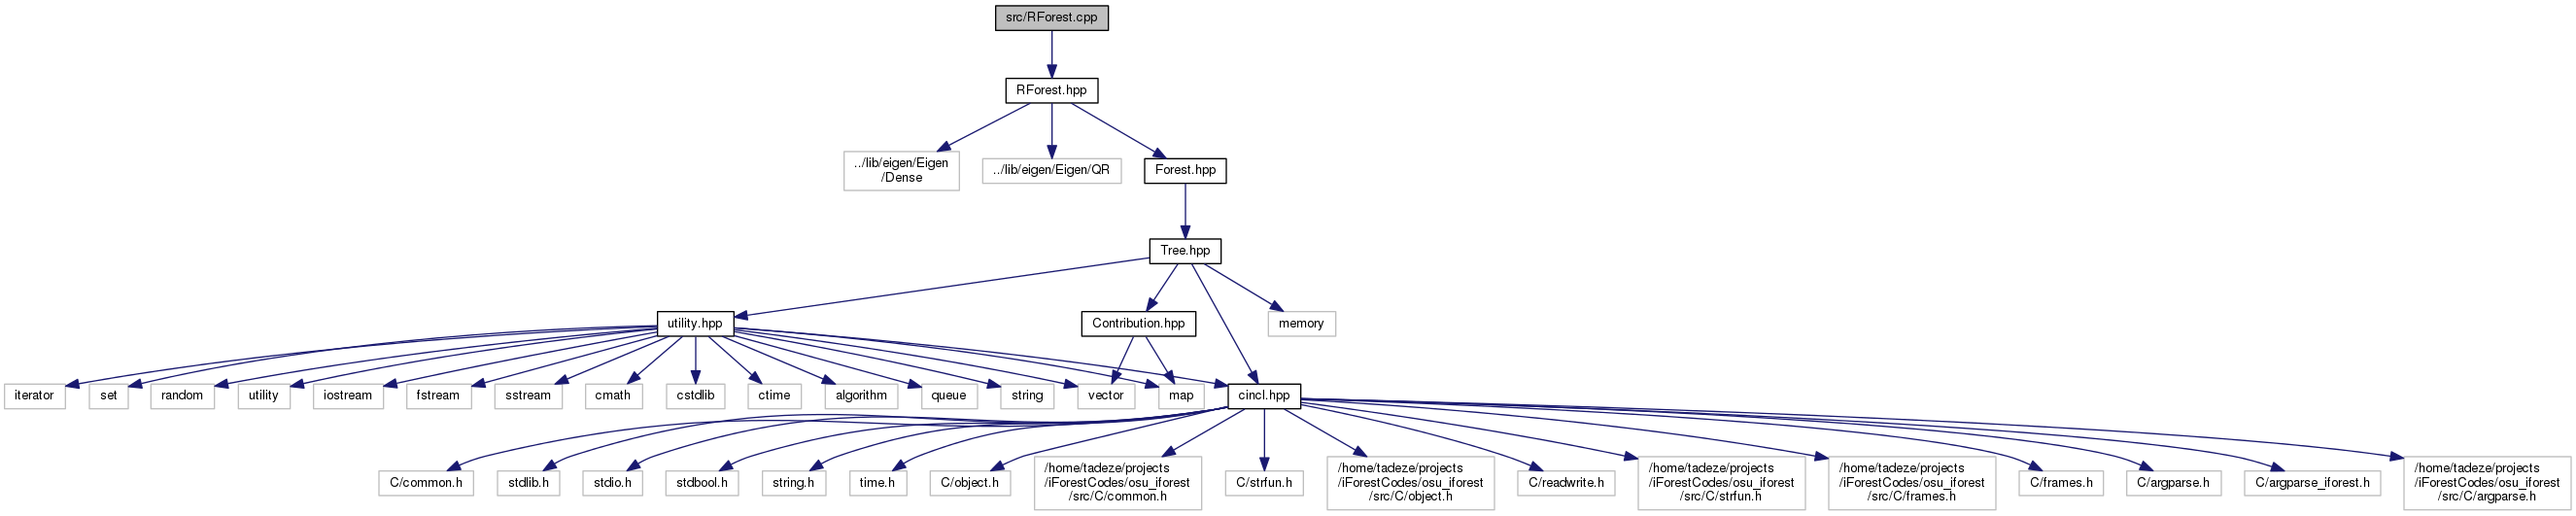
\includegraphics[width=350pt]{RForest_8cpp__incl}
\end{center}
\end{figure}

\hypertarget{RForest_8hpp}{}\section{src/\+R\+Forest.hpp File Reference}
\label{RForest_8hpp}\index{src/\+R\+Forest.\+hpp@{src/\+R\+Forest.\+hpp}}
{\ttfamily \#include \char`\"{}../lib/eigen/\+Eigen/\+Dense\char`\"{}}\newline
{\ttfamily \#include \char`\"{}../lib/eigen/\+Eigen/\+QR\char`\"{}}\newline
{\ttfamily \#include \char`\"{}Forest.\+hpp\char`\"{}}\newline
Include dependency graph for R\+Forest.\+hpp\+:\nopagebreak
\begin{figure}[H]
\begin{center}
\leavevmode
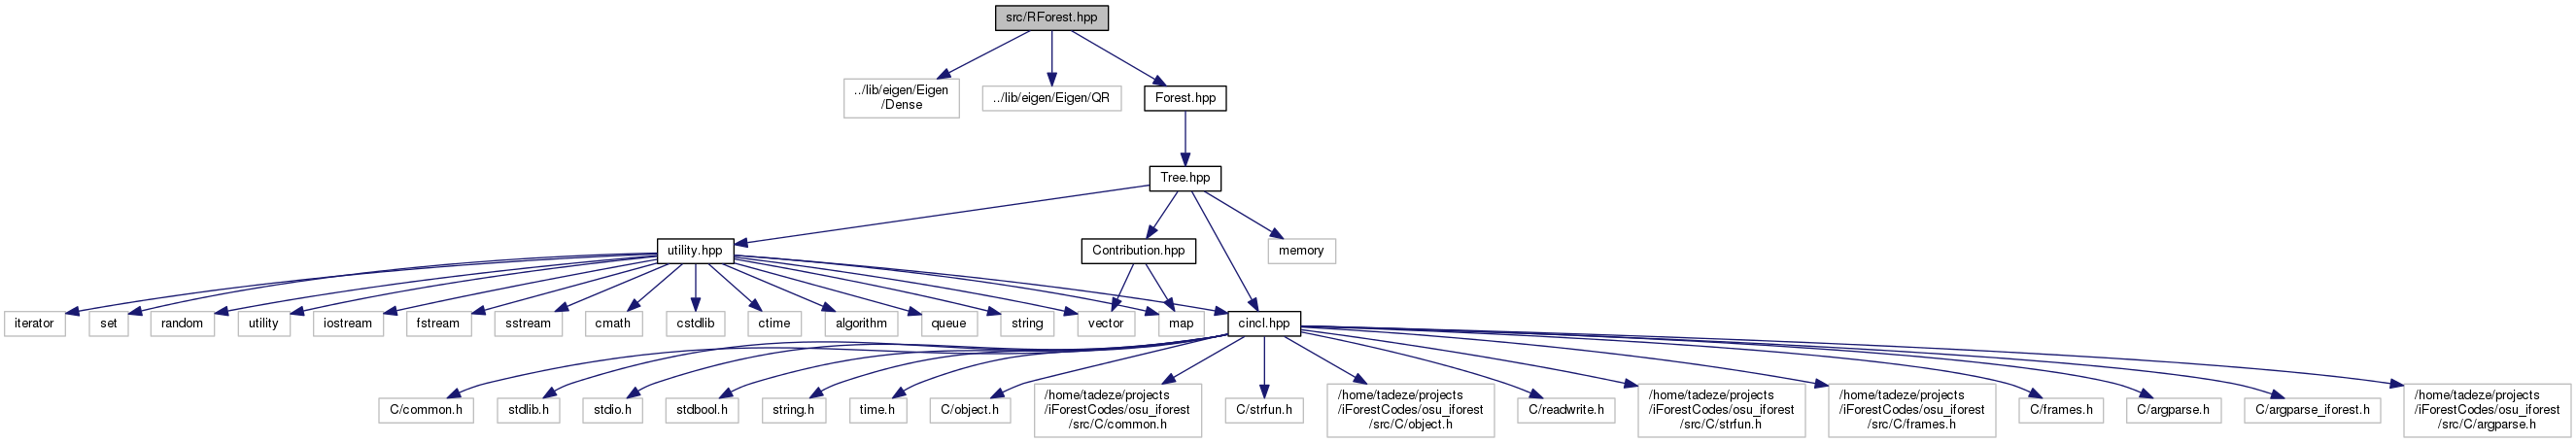
\includegraphics[width=350pt]{RForest_8hpp__incl}
\end{center}
\end{figure}
This graph shows which files directly or indirectly include this file\+:\nopagebreak
\begin{figure}[H]
\begin{center}
\leavevmode
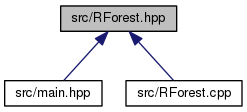
\includegraphics[width=257pt]{RForest_8hpp__dep__incl}
\end{center}
\end{figure}
\subsection*{Data Structures}
\begin{DoxyCompactItemize}
\item 
class \hyperlink{classRForest}{R\+Forest}
\end{DoxyCompactItemize}

\hypertarget{Tree_8cpp}{}\section{src/\+Tree.cpp File Reference}
\label{Tree_8cpp}\index{src/\+Tree.\+cpp@{src/\+Tree.\+cpp}}
{\ttfamily \#include \char`\"{}Tree.\+hpp\char`\"{}}\newline
Include dependency graph for Tree.\+cpp\+:\nopagebreak
\begin{figure}[H]
\begin{center}
\leavevmode
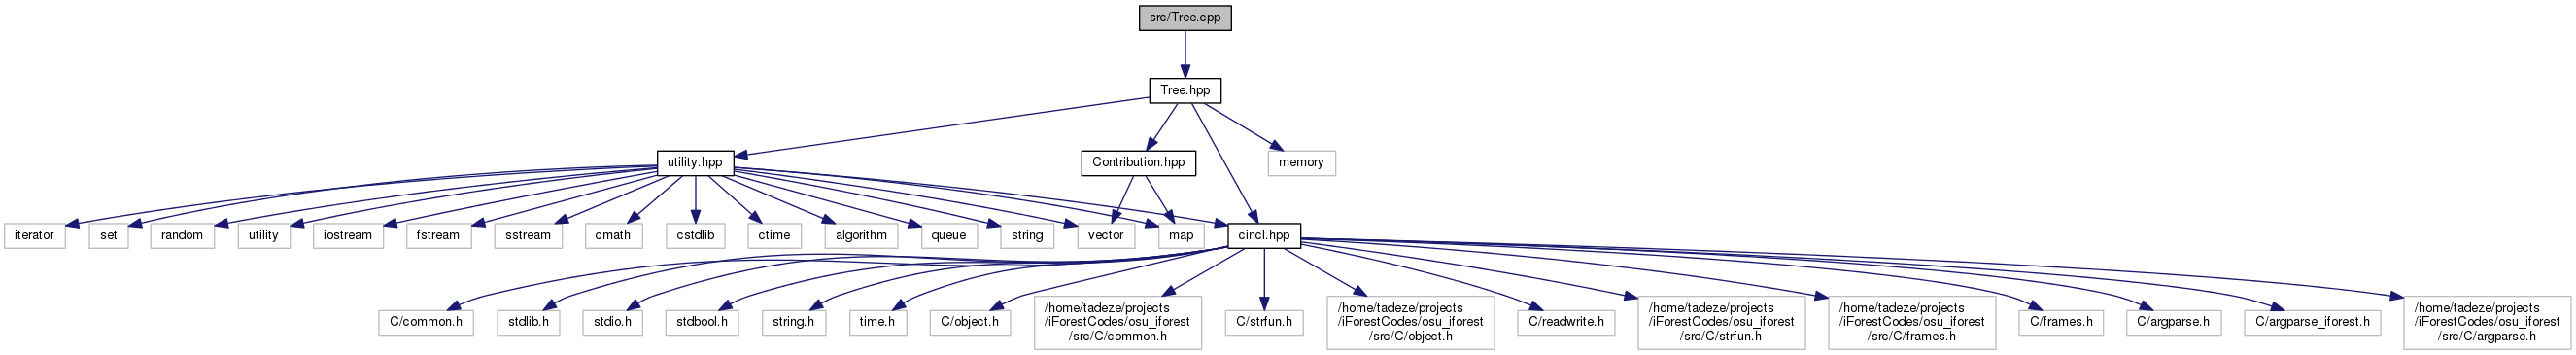
\includegraphics[width=350pt]{Tree_8cpp__incl}
\end{center}
\end{figure}

\hypertarget{Tree_8hpp}{}\section{src/\+Tree.hpp File Reference}
\label{Tree_8hpp}\index{src/\+Tree.\+hpp@{src/\+Tree.\+hpp}}
{\ttfamily \#include \char`\"{}utility.\+hpp\char`\"{}}\newline
{\ttfamily \#include \char`\"{}cincl.\+hpp\char`\"{}}\newline
{\ttfamily \#include \char`\"{}Contribution.\+hpp\char`\"{}}\newline
{\ttfamily \#include $<$memory$>$}\newline
Include dependency graph for Tree.\+hpp\+:\nopagebreak
\begin{figure}[H]
\begin{center}
\leavevmode
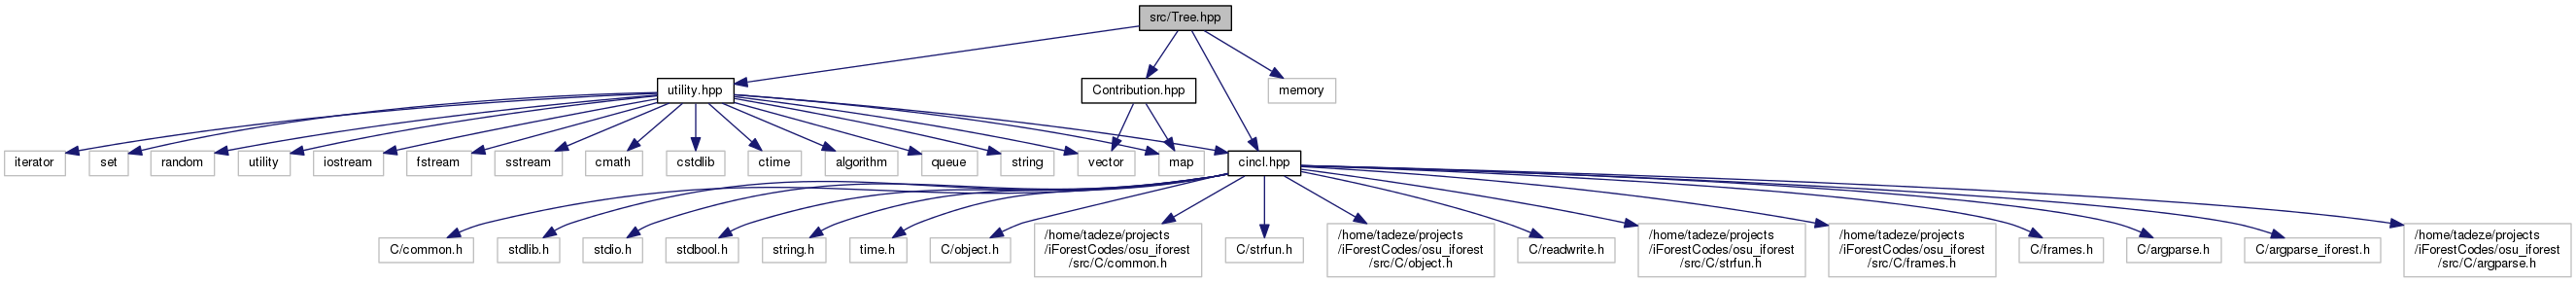
\includegraphics[width=350pt]{Tree_8hpp__incl}
\end{center}
\end{figure}
This graph shows which files directly or indirectly include this file\+:\nopagebreak
\begin{figure}[H]
\begin{center}
\leavevmode
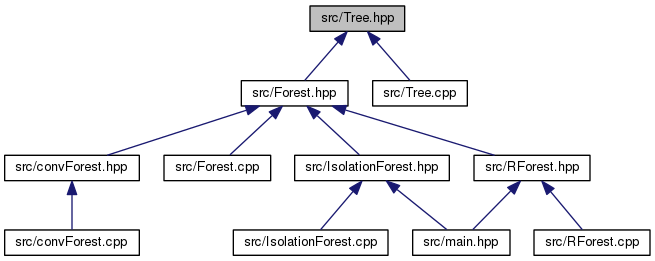
\includegraphics[width=350pt]{Tree_8hpp__dep__incl}
\end{center}
\end{figure}
\subsection*{Data Structures}
\begin{DoxyCompactItemize}
\item 
class \hyperlink{classTree}{Tree}
\end{DoxyCompactItemize}

\hypertarget{utility_8cpp}{}\section{src/utility.cpp File Reference}
\label{utility_8cpp}\index{src/utility.\+cpp@{src/utility.\+cpp}}
{\ttfamily \#include \char`\"{}utility.\+hpp\char`\"{}}\newline
Include dependency graph for utility.\+cpp\+:\nopagebreak
\begin{figure}[H]
\begin{center}
\leavevmode
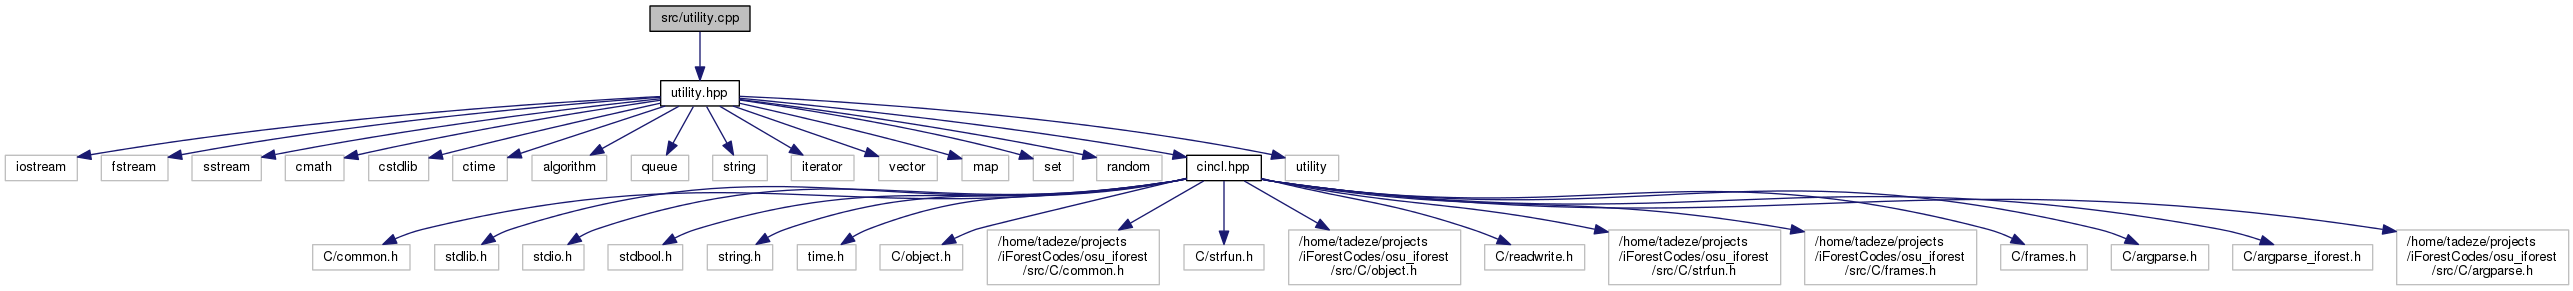
\includegraphics[width=350pt]{utility_8cpp__incl}
\end{center}
\end{figure}
\subsection*{Namespaces}
\begin{DoxyCompactItemize}
\item 
 \hyperlink{namespaceutil}{util}
\end{DoxyCompactItemize}
\subsection*{Functions}
\begin{DoxyCompactItemize}
\item 
void \hyperlink{namespaceutil_a60fc54ed78936dca89472845766b61f8}{util\+::initialize} ()
\item 
{\footnotesize template$<$typename T $>$ }\\T \hyperlink{namespaceutil_a254d46b3ebe9a685b6e0eca9db9d51ec}{util\+::randomT} (T min, T max)
\item 
double \hyperlink{namespaceutil_a1327645fe6fef26083bc9e1185b8d586}{util\+::randomD} (double min, double max)
\item 
int \hyperlink{namespaceutil_ab473893d6b386b2da951b72b4d40c085}{util\+::randomI} (int min, int max)
\item 
int \hyperlink{namespaceutil_a8751577b60f8e83b41c3cca32d65b677}{util\+::random\+Ex} (int min, int max, set$<$ int $>$ \&exlude)
\item 
void \hyperlink{namespaceutil_ab4e338c554526c6a942fc35d14b15beb}{util\+::sampleI} (int min, int max, int nsample, vector$<$ int $>$ \&samples)
\item 
double \hyperlink{namespaceutil_a71809e272f5a9c8e8297bab2c12666f7}{util\+::score} (double depth, int n)
\item 
{\footnotesize template$<$typename T $>$ }\\void \hyperlink{namespaceutil_a998845d03758baa45e52b967cf230b01}{util\+::swap\+Int} (int a, int b, T $\ast$x)
\item 
double \hyperlink{namespaceutil_afded8090794a80d2f1c9aa44e70c85ff}{util\+::mean} (vector$<$ double $>$ points)
\item 
double \hyperlink{namespaceutil_a43a50c7b5c6674cd27461d91cfec686c}{util\+::variance} (vector$<$ double $>$ \&x)
\item 
double \hyperlink{namespaceutil_a68758b62ab028fd0a2f0afb6d516be6f}{util\+::tconf} (vector$<$ double $>$ \&points, double sigma=0.\+95)
\item 
vector$<$ vector$<$ double $>$ $>$ \hyperlink{namespaceutil_a84b10f9fb76cc3f825e8c680ca7d786e}{util\+::readcsv} (const char $\ast$filename, char delim=\textquotesingle{},\textquotesingle{}, bool header=true)
\item 
map$<$ double, double $>$ \hyperlink{namespaceutil_ac7478c2543d3bf4901961c719ecc7d04}{util\+::ecdf} (vector$<$ double $>$ points)
\item 
{\footnotesize template$<$typename T $>$ }\\vector$<$ T $>$ \hyperlink{namespaceutil_a3da5afd362118ed04ca18ec46d5e6a96}{util\+::flatten} (const vector$<$ vector$<$ T $>$$>$ \&v)
\item 
double \hyperlink{namespaceutil_a1f106b9a1a65806393f73a3c8dbf01a6}{util\+::avg\+PL} (int n)
\item 
vector$<$ double $>$ \hyperlink{namespaceutil_a422abe670c555eeeded897e3d9861b77}{util\+::\+A\+Ddistance} (vector$<$ vector$<$ double $>$ $>$ depths, bool weight\+To\+Tail=false)
\item 
std\+::vector$<$ std\+::vector$<$ double $>$ $>$ \hyperlink{utility_8cpp_a840cdec08621ecfd4e68e2bfcb92f496}{synthetic\+Data} (int D, int N)
\end{DoxyCompactItemize}
\subsection*{Variables}
\begin{DoxyCompactItemize}
\item 
default\+\_\+random\+\_\+engine \hyperlink{namespaceutil_ab30b96cc3fcd37942fb7f9f8a2e1898d}{util\+::gen}
\end{DoxyCompactItemize}


\subsection{Function Documentation}
\mbox{\Hypertarget{utility_8cpp_a840cdec08621ecfd4e68e2bfcb92f496}\label{utility_8cpp_a840cdec08621ecfd4e68e2bfcb92f496}} 
\index{utility.\+cpp@{utility.\+cpp}!synthetic\+Data@{synthetic\+Data}}
\index{synthetic\+Data@{synthetic\+Data}!utility.\+cpp@{utility.\+cpp}}
\subsubsection{\texorpdfstring{synthetic\+Data()}{syntheticData()}}
{\footnotesize\ttfamily std\+::vector$<$std\+::vector$<$double$>$ $>$ synthetic\+Data (\begin{DoxyParamCaption}\item[{int}]{D,  }\item[{int}]{N }\end{DoxyParamCaption})}


\hypertarget{utility_8hpp}{}\section{src/utility.hpp File Reference}
\label{utility_8hpp}\index{src/utility.\+hpp@{src/utility.\+hpp}}
{\ttfamily \#include $<$iostream$>$}\newline
{\ttfamily \#include $<$fstream$>$}\newline
{\ttfamily \#include $<$sstream$>$}\newline
{\ttfamily \#include $<$cmath$>$}\newline
{\ttfamily \#include $<$cstdlib$>$}\newline
{\ttfamily \#include $<$ctime$>$}\newline
{\ttfamily \#include $<$algorithm$>$}\newline
{\ttfamily \#include $<$queue$>$}\newline
{\ttfamily \#include $<$string$>$}\newline
{\ttfamily \#include $<$iterator$>$}\newline
{\ttfamily \#include $<$vector$>$}\newline
{\ttfamily \#include $<$map$>$}\newline
{\ttfamily \#include $<$set$>$}\newline
{\ttfamily \#include $<$random$>$}\newline
{\ttfamily \#include \char`\"{}cincl.\+hpp\char`\"{}}\newline
{\ttfamily \#include $<$utility$>$}\newline
Include dependency graph for utility.\+hpp\+:\nopagebreak
\begin{figure}[H]
\begin{center}
\leavevmode
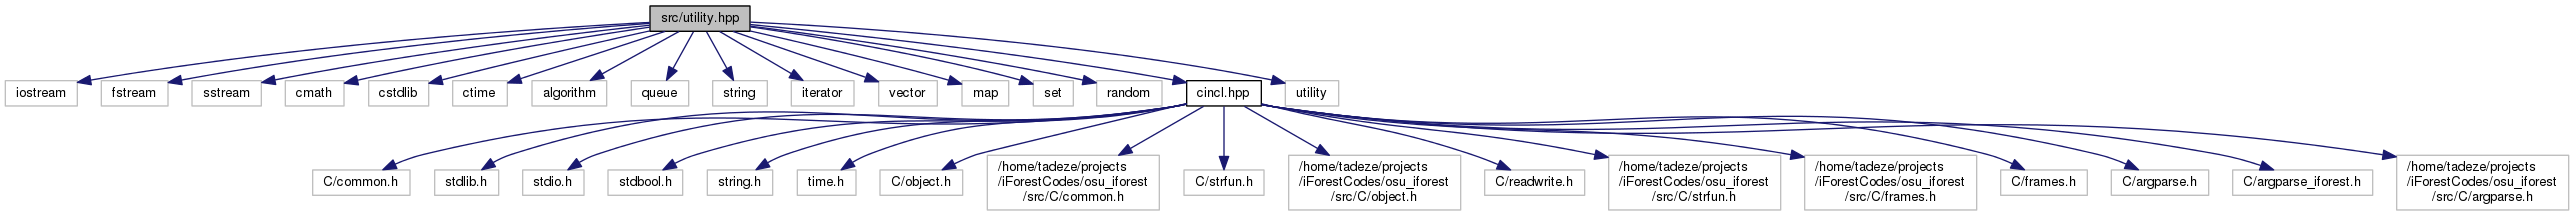
\includegraphics[width=350pt]{utility_8hpp__incl}
\end{center}
\end{figure}
This graph shows which files directly or indirectly include this file\+:\nopagebreak
\begin{figure}[H]
\begin{center}
\leavevmode
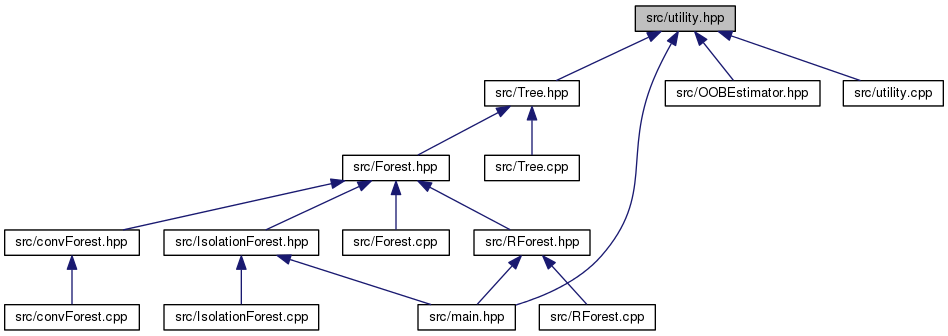
\includegraphics[width=350pt]{utility_8hpp__dep__incl}
\end{center}
\end{figure}
\subsection*{Data Structures}
\begin{DoxyCompactItemize}
\item 
class \hyperlink{classutil_1_1Matrix}{util\+::\+Matrix$<$ T $>$}
\end{DoxyCompactItemize}
\subsection*{Namespaces}
\begin{DoxyCompactItemize}
\item 
 \hyperlink{namespaceutil}{util}
\end{DoxyCompactItemize}
\subsection*{Functions}
\begin{DoxyCompactItemize}
\item 
void \hyperlink{namespaceutil_a60fc54ed78936dca89472845766b61f8}{util\+::initialize} ()
\item 
int \hyperlink{namespaceutil_ab473893d6b386b2da951b72b4d40c085}{util\+::randomI} (int min, int max)
\item 
int \hyperlink{namespaceutil_ae080f004741b0ea81032b3ec0c723f4c}{util\+::random\+Ex} (int min, int max, std\+::set$<$ int $>$ \&exlude)
\item 
void \hyperlink{namespaceutil_a077f5faad89062a4013dc98fc85b7a40}{util\+::sampleI} (int min, int max, int nsample, std\+::vector$<$ int $>$ \&sample\+Indx)
\item 
double \hyperlink{namespaceutil_a1f106b9a1a65806393f73a3c8dbf01a6}{util\+::avg\+PL} (int n)
\item 
double \hyperlink{namespaceutil_a1327645fe6fef26083bc9e1185b8d586}{util\+::randomD} (double min, double max)
\item 
{\footnotesize template$<$typename T $>$ }\\T \hyperlink{namespaceutil_a254d46b3ebe9a685b6e0eca9db9d51ec}{util\+::randomT} (T min, T max)
\item 
void \hyperlink{namespaceutil_a8a222a481a56e4070f023d369483f707}{util\+::swap\+Int} (int a, int b, int $\ast$x)
\item 
double \hyperlink{namespaceutil_a2f9d2ca343c1e5fcbc1da5140de61f94}{util\+::variance} (std\+::vector$<$ double $>$ \&x)
\item 
double \hyperlink{namespaceutil_a67baa21858f5d569c1553bb179da7115}{util\+::mean} (std\+::vector$<$ double $>$ points)
\item 
double \hyperlink{namespaceutil_a0b673442b1c87f0daf8bb0a4179a6834}{util\+::tconf} (std\+::vector$<$ double $>$ \&points, double sigma)
\item 
vector$<$ vector$<$ double $>$ $>$ \hyperlink{namespaceutil_a84b10f9fb76cc3f825e8c680ca7d786e}{util\+::readcsv} (const char $\ast$filename, char delim=\textquotesingle{},\textquotesingle{}, bool header=true)
\item 
std\+::map$<$ double, double $>$ \hyperlink{namespaceutil_abfb0e38d71ca69f5f6a505b3f5f7dc52}{util\+::ecdf} (std\+::vector$<$ double $>$ points)
\item 
std\+::vector$<$ double $>$ \hyperlink{namespaceutil_a08fbdd196c73244d0e2130c3a70d2f2b}{util\+::\+A\+Ddistance} (const std\+::vector$<$ std\+::vector$<$ double $>$ $>$ \&depths, bool weight\+To\+Tail)
\item 
double \hyperlink{namespaceutil_a71809e272f5a9c8e8297bab2c12666f7}{util\+::score} (double depth, int n)
\end{DoxyCompactItemize}
\subsection*{Variables}
\begin{DoxyCompactItemize}
\item 
std\+::ofstream \hyperlink{namespaceutil_af123fd54ef9ea843e69a69dfd986f59e}{util\+::logfile}
\item 
std\+::string \hyperlink{namespaceutil_a4839a6e82a650d17fe48a7ab99640835}{util\+::tmp\+Var}
\item 
int \hyperlink{namespaceutil_aeda4e5339822ac6c9fb3f1991c126bfb}{util\+::debug}
\end{DoxyCompactItemize}

%--- End generated contents ---

% Index
\backmatter
\newpage
\phantomsection
\clearemptydoublepage
\addcontentsline{toc}{chapter}{Index}
\printindex

\end{document}
